%%%%%%%%%% FRENCH MANUAL %%%%%%%%%%%%%%%%%
\documentclass[a4paper,11pt]{book}
\usepackage[utf8]{inputenc}
\usepackage{amsfonts,amsmath,amssymb,mathrsfs}
\usepackage{makeidx}
\usepackage[french]{babel}
\usepackage[T1]{fontenc}
\usepackage{graphicx,ulem}
\usepackage{multicol,longtable,array}
\usepackage{colortbl,color}
\usepackage{pstricks,pstricks-add,pst-math,pst-xkey}
\usepackage{geometry}
\geometry{a4paper,tmargin=2cm,bmargin=2cm,rmargin=1.5cm,lmargin=1.5cm}
\newcommand{\logo}{\textsc{Logo}}
\newcommand{\xlogo}{\textsc{XLogo}}
\newcommand{\prim}[2]{
\\
\noindent \begin{tabular}{>{\columncolor[gray]{0.9}}p{\textwidth}} 
\ifx \Css\UnDef\else
\Css{\#TBL-\TableNo {width:100\%;} }
\fi
\index{#1} \textbf{#1} \textit{#2}\\ 
\end{tabular} 
\\ 
}
\author{Loïc Le Coq}
\title{
\Huge \textbf{\xlogo: Manuel de référence} 
}
\date{\today
\begin{center}
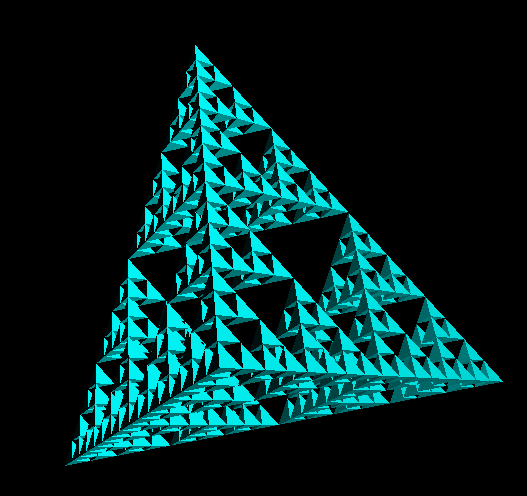
\includegraphics[scale=0.8]{images/title.png}
\end{center}
\texttt{http://xlogo.tuxfamily.org}\\
}
\makeindex
\begin{document} 
\renewcommand{\labelitemi}{\textbullet}
\renewcommand{\labelitemiii}{$\rightarrow$}
\maketitle
\chapter{Introduction}
\logo\ is a programming language developed in the 1960's by Seymour Papert. Papert was the developer of an original and highly influential theory on learning called ``constructionism'' which could be summarised with the expression: ``learning by doing''.\\ \\
\logo\ is a really good language to develop mathematical and logic skills. It is an excellent language to begin learning with, as it teaches the basics of things like loops, tests, procedures, etc. The user moves an object called a "turtle" around the screen using commands as simple as forward, back, right, and so on. As it moves, the turtle leaves a trail behind it, and so it is therefore possible to create drawings. The fact that the user can give the turtle orders in a very natural language makes \logo\ very easy to learn. More advanced usage is possible too with operations on lists, words or files.\\ \\
\xlogo\ is a \logo\ interpreter, it means that the user's instructions are executed directly. The user can see their errors on screen immedately. This very intuitive graphical approach makes Logo an ideal language for beginners, especially children!\\ \\
The main adress for the \xlogo website is
\begin{center}
\texttt{http://xlogo.tuxfamily.org/}
\end{center}
Here you can download both the documentation and the software. You can also find many examples created with \xlogo\ and you will be able to judge \xlogo's capacity.\\ \\
\xlogo\ now supports ten languages (arabic, asturian, english, esperanto, french, galician, greek, german, portuguese and spanish) and is written in \textsc{Java} - a programming language with the benefit of being cross-platform. Therefore \xlogo\ will run on Linux, Windows or MacOS machines without problems.\\ \\
\xlogo\  is licensed under the GPL: Hence, it is free software and users have four freedoms:
\begin{itemize}
\item Freedom 1: The freedom to run the program for any purpose.
\item Freedom 2: The freedom to study and modify the program.
\item Freedom 3: The freedom to copy the program so you can help your neighbour.
\item Freedom 4: The freedom to improve the program, and release your improvements to the public, so that the whole community benefits.
\end{itemize}
\vspace{0.3cm}
\noindent \textbf{Manual structure:}\\ \\
This manual will help you to discover \xlogo.
\begin{itemize}
 \item In the first part, different menus and interface options are explained.
 \item Then, some chapters presenting the most important instructions to begin using \xlogo. The first are very easy and then, complexity grows. Sometimes, at the end of a chapter, some exercices are presented. Their solutions can be found in appendix D.
\item Then, a sequence of different themes is offered for advanced users.
\item In appendix A, you'll find a complete description of all \xlogo's primitives.
\end{itemize}
\vspace{0.5cm}
This manual exists under several formats:
\begin{itemize}
 \item \textsc{PDF}: http://downloads.tuxfamily.org/xlogo/downloads-en/manual-en.pdf
 \item \textsc{Zipped HTML}: http://downloads.tuxfamily.org/xlogo/downloads-en/manual-html-en.zip
 \item \LaTeXe: Manual Source: http://downloads.tuxfamily.org/xlogo/downloads-fr/manual-src-en.zip
 \item \textsc{JavaHelp}: Menu Help-Online Manual in \xlogo
\end{itemize}

\tableofcontents
\chapter{Installare \xlogo}
\noindent \begin{itemize}
 \item Prima di tutto occorre installare la Java Runtime Environment (JRE) sul proprio computer. Vai a questa pagina:
\begin{center}
\texttt{ http://java.sun.com/javase/downloads/index.jsp}
\end{center}
Scarica la JRE corrispondente al proprio sistema operativo (Windows, Linux, MacOS), ed installala. 
\item Quindi occorre scaricare il file \texttt{xlogo.jar} dal seguente indirizzo: 
\begin{center}
	\texttt{http://xlogo.tuxfamily.org/common/xlogo.jar}
\end{center}
In alternativa si può andare sul sito web di \xlogo\, all'indirizzo \texttt{http://xlogo.tuxfamily.org}, scegliere una lingua e quindi cliccare sulla voce di menu Download.
\end{itemize}
\section{Configurazione di \xlogo}
\subsection{Ambiente Linux}
\textbf{Nota:} \xlogo\ è già incluso nella distribuzione OpenSuse.\\
In Ubuntu 8.04:
\begin{enumerate}
 \item Per installare la JRE:
\begin{itemize}
 \item Sistema -> Amministrazione -> Gestore Pacchetti Synaptic
 \item Installare il pacchetto \texttt{sun-java6-jre}
\end{itemize}
 \item  Per aprire il file \texttt{xlogo.jar}:
\begin{itemize}
 \item Clicca il tasto destro del mouse su \texttt{xlogo.jar}, Proprietà
 \item Tab ``Apri con'': Scegli Sun Java 6 Runtime 
\end{itemize}
 \item Per associare l'estensione \texttt{lgo} a \xlogo:
\begin{itemize}
 \item Clicca il tasto destro del mouse su \texttt{xlogo.jar}, Proprietà
 \item Tab ``Apri con'' 
 \item Bottone ``Aggiungi''
 \item Campo ``Usare un comando personalizzato'', digita (sostituendo il percorso verso \xlogo\ a ``percorso\_a\_''):
\begin{center}
\texttt{java -jar percorso\_a\_xlogo.jar} 
\end{center}
\end{itemize}
\end{enumerate}

\subsection{Ambiente Windows}
In teoria, se clicchi sull'icona di \xlogo\ il programma dovrebbe partire.
Se \xlogo\ parte correttamente, salta il resto del capitolo. Se invece viene lanciata un'altra applicazione (per esempio winzip) questo succede poiché i file .jar vengono interpretati come file .zip (ossia compressi) e viene eseguito il programma per la loro decompressione. Occorre quindi deattivare l'associazione di quel programma con i file .jar. Per far questo segui i seguenti passi per Windows XP (alcuni percorsi potrebbero essere diversi a seconda della versione di Windows in funzione, dovrai modificarli appropriatamente):

\begin{enumerate}
\item Avvio -> Pannello di controllo -> Passa alla modalità classica  -> Opzioni cartella
\item Clicca sul Tab ``Tipi di file'' (il terzo Tab)
\item Cerca nella lista dei file registrati, quelli connessi con i file jar (file jar, file jar eseguibili, archivi jar, ecc)
\item Clicca il tipo di file, quindi su Avanzate
\item Appare una nuova finestra, clicca su Sfoglia...
\item Naviga verso javaw.exe che di solito è posto presso:
\begin{center}
\texttt{c:\textbackslash{}Programmi \textbackslash{}java\textbackslash{}j2re1.4.1\textbackslash{}bin\textbackslash{}javaw.exe}
\end{center}
\item Il percorso {}``c:\textbackslash{}Programmi \textbackslash{}java\textbackslash{}j2re1.4.1\textbackslash{}bin\textbackslash{}javaw.exe'' appare quindi nel campo \textit{Applicazione utilizzata per eseguire l'azione:}. Occorre aggiungere delle informazioni alla sua fine così che si legga:
\begin{center}
\texttt{ "c:\textbackslash{}Program Files\textbackslash{}java\textbackslash{}j2re1.4.1\textbackslash{}bin\textbackslash{}javaw.exe" -jar {}"\%1" \%{*}}
\end{center}
(nota che c'è uno spazio su entrambi i lati di -jar).
\item Infine, chiudi tutte le finestre di dialogo. Ora tutto ciò che rimare da fare è cliccare sull'icona di \xlogo\ per lanciarlo!
\end{enumerate}
Se ancora \xlogo\ non parte, c'è una seconda possibilità. Apri una finestra MSDOS (su XP: Avvio -> Tutti i programmi -> Accessori -> Prompt dei comandi), quindi digitare il seguente comando (sostituendo il percorso verso \xlogo\ a ``percorso\_a\_''):
\begin{center}
\begin{verbatim}
java -jar percorso_a_XLogo

Per esempio: java -jar c:\windows\office\xlogo.jar

\end{verbatim}
(se \texttt{xlogo.jar} è posto in questa cartella).

\end{center}

Se digitare questo comando ogni volta è troppo lungo, crea un file di nome (per esempio) xlogo.bat ed inseriscici il comando stesso. Puoi quindi cliccare su questo file per lanciare \xlogo.

\subsubsection*{Associare i file con estensione .lgo a XLogo}
I file con estensione .lgo non sono di solito riconosciuti dal sistema operativo e quando si clicca su uno di loro una finestra di dialogo appare richiedendo di selezionare un'applicazione per aprirli. Selezionare \texttt{Altro} e quindi fornire il percorso a \texttt{javaw.exe} \begin{center}
Di solito è: \texttt{C:\textbackslash{}Programmi \textbackslash{}java\textbackslash{}j2re1.4.1\textbackslash{}bin\textbackslash{}javaw.exe}
\end{center}  
Viene quindi chiesto di inserire un nome per designare i file con l'estensione \texttt{.lgo}.\\
Per esempio: \texttt{File XLogo}\\
Per impostarlo come default in Windows XP, segui i seguenti passi:

\begin{enumerate}
\item Avvio -> Pannello di controlo -> Passa alla modalità classica  -> Opzioni cartella
\item Clicca sul Tab ``Tipi di file'' (il terzo Tab)
\item Cerca nella lista dei file registrati, quelli connessi con i file jar (file jar, file jar eseguibili, archivi jar, ecc)
\item Clicca il tipo di file, quindi su Nuovo
\item Digita l'estensione .lgo nel riquadro Estensione File e clicca OK
\item Clicca nella riga LGO appena aggiunta nell'elenco nei tipi di file registrati e clicca Avanzate
\item Apapre una nuova finestra, clicca su Nuovo
\item Sotto Azioni, inserisci ``apri" e quindi clicca su Sfoglia... naviga perso javaw.exe che, usualmente è in
\begin{center}
\texttt{c:\textbackslash{}Programmi \textbackslash{}java\textbackslash{}j2re1.4.1\textbackslash{}bin\textbackslash{}javaw.exe}
\end{center}
\item Clicca su Apri per aggiungere il percorso al riquadro Azioni della fienstra di dialogo Modifica Tipo di file.
\item Clicca su apri quindi su modifica
\item Il persorso {}``c:\textbackslash{}Programmi \textbackslash{}java\textbackslash{}j2re1.4.1\textbackslash{}bin\textbackslash{}javaw.exe'' appare quindi nel campo \textit{Applicazione utilizzata per eseguire l'azione:}. Occorre aggiungere delle informazioni alla sua fine così che si legga:
\begin{center}
\texttt{\textquotedbl c:\textbackslash{}Program Files\textbackslash{}java\textbackslash{}j2re1.4.1\textbackslash{}bin\textbackslash{}javaw.exe\textquotedbl  -jar {}"\%1" \%{*}}
\end{center}
\item Infine, chiudi tutte le finestre di dialogo. Ora tutto ciò che rimare da fare è cliccare sull'icona d el file lgo per lanciare \xlogo\r!
\end{enumerate}

\section{Aggiornamenti \xlogo}
\begin{center}

\includegraphics{pics/rss.png} \hspace{1cm} \texttt{http://xlogo.tuxfamily.org/rss.xml}
\end{center}
Per aggiornare \xlogo, occorre semplicemente rimpiazzare il file \texttt{xlogo.jar} con la nuova versione. 
Se vuoi ricevere un avviso quando viene pubblicata una nuova versione puoi abbonarti al feed RSS di \xlogo. L'indirizzo è 
\begin{center}
 \texttt{http://xlogo.tuxfamily.org/rss.xml}
\end{center}
Molti programmi possono gestire gli abbonamenti RSS. Se non ti senti a tuo agio con questa tecnica la scelta più facile è usare Mozilla Thunderbird:
\begin{itemize}
 \item Menu Modifica - Impostazioni Account
 \item Bottone ``Aggiungi account''
 \item ``News RSS \& Blog'', Next
 \item Nome Account: ``Feed RSS'' per esempio
 \item Bottoni ``Continua'' e ``Fine''
 \item Nella finestra principale ``Impostazioni Account'', Seleziona ``Feed RSS'' nel menu di sinistra e clicca sul bottone ``Gestione Sottoscrizioni''.
 \item Bottone ``Aggiungi''
	\begin{itemize}
 	\item URL del Feed: \texttt{http://xlogo.tuxfamily.org/rss.xml}
	\item Seleziona l'oggetto ``Mostra il sommario dell'articolo invece di caricare la pagina web''
	\end{itemize}
\end{itemize}
\vspace*{0.2cm}
È finita, con il bottone ``Ricevi posta'', puoi ricevere le news \xlogo\ insieme alle email.
\section{Disinstallazione}\label{fichier_perso}
Per disinstallare \xlogo, tutto ciò che occore fare è cancellare il file \texttt{xlogo.jar} ed il file di configurazione \texttt{.xlogo}\label{file_perso}, che è posto nella cartella home dell'utente (\texttt{/home/account} per gli utenti Linux, o \texttt{c:\textbackslash windows\textbackslash.xlogo} per gli utenti Windows).

\chapter{Descrizione dell'interfaccia}
\section{Prima esecuzione}
La prima volta che \xlogo\ viene lanciato (o se il file \texttt{.xlogo} è stato cancellato -Leggi la sezione  \ref{file_perso}-) una finestra di dialogo appare per chiedere di definire la lingua di utilizzo del programma stesso e dei programmi logo che con esso si realizzeranno.
\begin{center}
	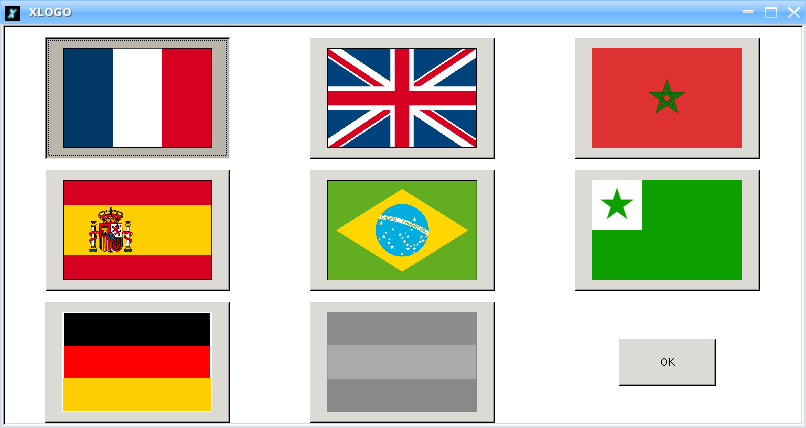
\includegraphics[scale=0.2]{pics/interface-CaptureLangue.png} 
\end{center}
La lingua predefinita può essere cambiata in qualsiasi momento nella finestra delle Preferenze (Sezione  \ref{general_tab}).
\section{La finestra principale}
\begin{center}
	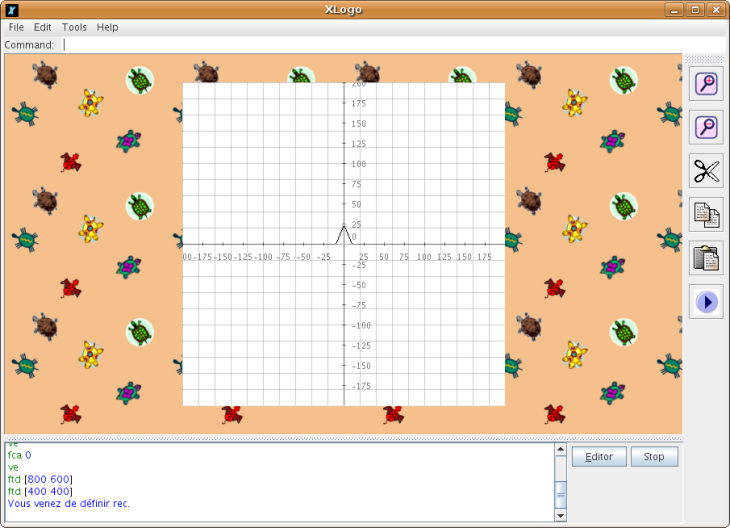
\includegraphics[  scale=0.4]{pics/interface-Capture.png} 
\end{center}

\begin{itemize}
	\item Nella parte superiore vi sono i menu usuali \textbf{File Modifica Strumenti e Aiuto}
	\item Appena al sotto è collocata la \textbf{linea di comando}, che permette alle istruzioni logo di essere eseguite.
	\item Nella parte centrale dello schermo vi è l'\textbf{area di disegno}. 
	\item Sulla destra dell'area di disegno una \textbf{barra degli strumenti} permette all'utente di eseguire numerose azioni:
	\begin{itemize}
		\item Ingrandire e rimpicciolire.
		\item Modifica (taglia/copia/incolla)
		\item Il bottone ``avvia'' lancia il comando principale definito nell'editor.
	\end{itemize}
	\item Nella parte inferiore vi è lo \textbf{storico dei comandi} che mostra tutti i comandi inseriti e la risposta associata dell'interprete. Per richiamare velocemente un comando che è stato già inserito ci sono due opzioni: o si clicca sul vecchio comando nello storico o si può cliccare sulla bassa di scorrimento finché il vecchio comando appare nell'elenco. La barra di scorrimento permette di navigare attraverso tutti i comandi inseriti (molto pratico). 
	\item Alla destra dello storico ci sono due bottoni: \textbf{STOP} e \textbf{EDITOR}. 
	\begin{itemize}
		\item Il bottone STOP interrompe l'esecuzione del programma logo.
		\item Il bottone EDITOR apre la l'editor delle procedure.\\ 
	\end{itemize}
\end{itemize}
\section{L'editor delle procedure}
\begin{center}
	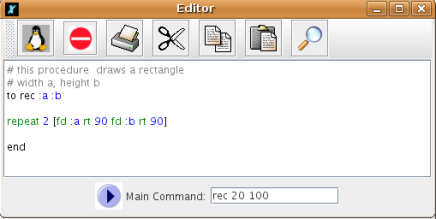
\includegraphics[scale=0.4]{pics/interface-CaptureEditor.png}
\end{center}
Esistono tre modi per aprire l'editor:\\
\begin{itemize}
	\item Digita \texttt{ed} sulla linea di comando nella parte superiore dello schermo. L'editor si apre mostrando tutte le procedure già definite. Se si vuole modificare una o più procedure specifiche digitare:\\
	\texttt{ed {[}procedura\_1 procedura\_2 $\ldots$]}
	\item Premi il bottone Editor nello schermo principale. 
	\item Premi i tasti Alt+E sulla tastiera. 
\end{itemize}
I seguenti sono i vari bottoni che si trovano nell'editor:\\

\begin{longtable}{cm{12cm}}
	\includegraphics*[scale=1]{pics/interface-turtle.png} &
	Salva i cambiamenti effettuati nell'editor e ne chiude la finestra. È questo il bottone che occorre premere ogni volta per inserire le nuove procedure digitate. È possibile anche premere i tasti Alt+Q sulla tastiera.\\
	\includegraphics*[scale=1]{pics/interface-quit.png}&
	Chiude la finestra dell'editor senza salvare i cambiamenti effettuati. È possibile anche premere i tasti Alt+C sulla tastiera.\\
	\includegraphics*[scale=1]{pics/interface-fileprint.png}&
	Stampa il contenuto dell'editor.\\
	\includegraphics*[scale=1]{pics/interface-editcopy.png}&
	Copia il testo selezionato negli appunti.\\
	\includegraphics*[scale=1]{pics/interface-editcut.png}&
	Taglia il testo selezionato negli appunti.\\
	\includegraphics*[scale=1]{pics/interface-editpaste.png}&
	Incolla il testo selezionato negli appunti.\\
	\includegraphics*[scale=1]{pics/interface-chercher.png}&
	Apri un riquadro per Cercare/Sostituire del testo nell'editor.\\
\end{longtable}
\begin{center}
	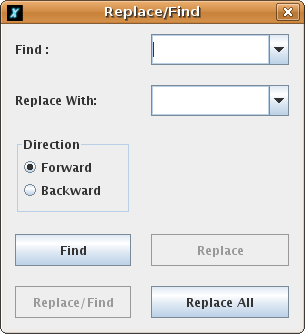
\includegraphics[scale=0.4]{pics/interface-CaptureFind.png}
\end{center}
\vspace{0.5cm}

\includegraphics{pics/interface-play.png}
Nella farte inferiore dell'editor un campo di testo permette di definire un comando principale. Questo comando è l'istruzione generale che lancia il programma logo. Può essere acceduta tramite il bottone ``Avvia'' dalla barra degli strumenti della finestra principale. Questo comando viene salvato e caricato insieme al programma logo (con estensione \texttt{.lgo}) viene salvato tramite l'editor. \\ \\
\textbf{\begin{Large}IMPORTANTE\end{Large}} \\
\begin{itemize}
	\item Da notare che cliccando sul bottone di chiusura della finestra dell'editor (x), l'editor non si chiuderà! Solo uno dei due bottoni principale consente la chiusura dell'editor. 
	\item Per cancellare una o più procedure occorre usare le primitive \texttt{CancProc} e \texttt{CancTutte} nella linea di comando, o usare il gestore delle procedure che si trova nel menu Strumenti.
\end{itemize}
\section{Chiudere \xlogo}
Per chiudere \xlogo, si può scegliere \textbf{File - Abbandona} nella barra dei menu, o cliccare sul bottone di chiusura nella barra del titolo della finestra. una finestra di dialogo chiede quindi di confermare la chiusura del programma.\\
\textbf{Nota per l'ambiente Mac}. In ambiente Mac è preferibile non utilizzare la funzione di chiusura dell'applicazione presente di default nella barra dei menu fornita da Mac OS ma utilizzare i due metodi esposti al paragrafo precedente.
\begin{center}
	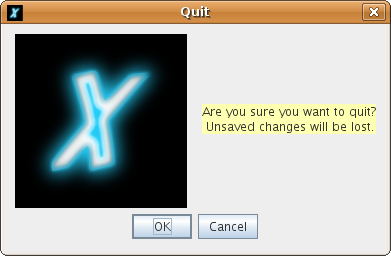
\includegraphics[scale=0.4]{pics/interface-CaptureQuit.png}
\end{center}





\chapter{Opzioni del menu}

\section{Menu ``File''}
\begin{itemize}
	\item \textbf{File$\to$Nuovo}: crea un nuovo ambiente di lavoro, cancella tutte le procedure e variabili.
	\item \textbf{File$\to$Apri}: apre un file logo precedentemente salvato.
	\begin{center}
		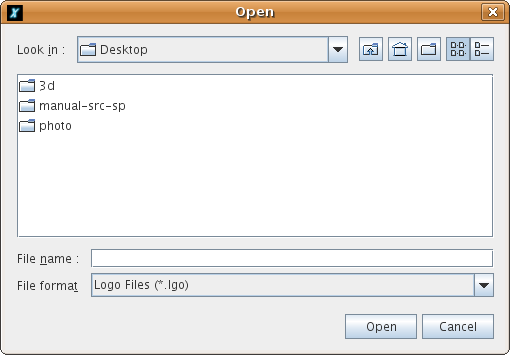
\includegraphics[scale=0.4]{pics/interface-CaptureOpen.png}
	\end{center}
	\vspace{0.25cm}
	\item \textbf{File$\to$Registra come\textellipsis} salva le procedure correnti con un nome diverso.
	\begin{center}
		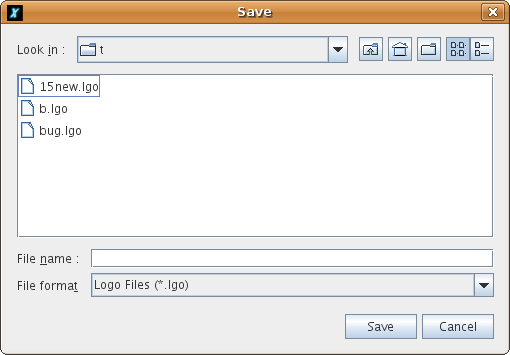
\includegraphics[scale=0.4]{pics/interface-CaptureSave.png}
	\end{center}
	\vspace{0.25cm}
	\item \textbf{File$\to$Registra}: salva le procedure nel file corrente
	\item \textbf{File$\to$Cattura$\to$Registra come\textellipsis}: permette di salvare l'immagine dell'area di disegno in formato jpeg o png. Se vuoi registrare solo una parte dell'immagine puopi definire un'area rettangolare trascinando il mouse sull'area di disegno.
	\vspace{0.25cm}
	\item \textbf{File$\to$Cattura$\to$Stampa\textellipsis}: permette di stampare l'immagine o parte di essa.
	\item \textbf{File$\to$Cattura$\to$Copia Appunti}: copia l'immagine o parte di essa negli appunti di sistema. Funziona in ambiente Windows e Mac OS, non in Linux (gli appunti hanno un comportamento diverso).
	\item \textbf{File$\to$Testo$\to$Registra come\textellipsis (formato RTF)}: registra lo storico dei comandi in formato RTF (preservando colori e formati).
	\item \textbf{File$\to$Abbandona}: esce da \xlogo.
\end{itemize}

\section{Menu ``Modifica''}
\begin{itemize}
	\item \textbf{Modifica$\to$Copia}: copia il testo selezionato negli appunti.
	\item \textbf{Modifica$\to$Taglia}: taglia il testo selezionato negli appunti.
	\item \textbf{Modifica$\to$Incolla}: Incolla il testo degli appunti nella linea di comando.
	\item \textbf{Modifica$\to$Selezina tutto}: Seleziona tutto il testo nella linea di comando.
\end{itemize}

\section{Menu ``Strumenti''}
\begin{itemize}
	\item \textbf{Strumenti$\to$Colore Penna}: permette di impostare il colore della penna della tartaruga scegliendo da una gamma di colori. E' anche accessibile dal comando \texttt{ImpCP}.
	\begin{center}
		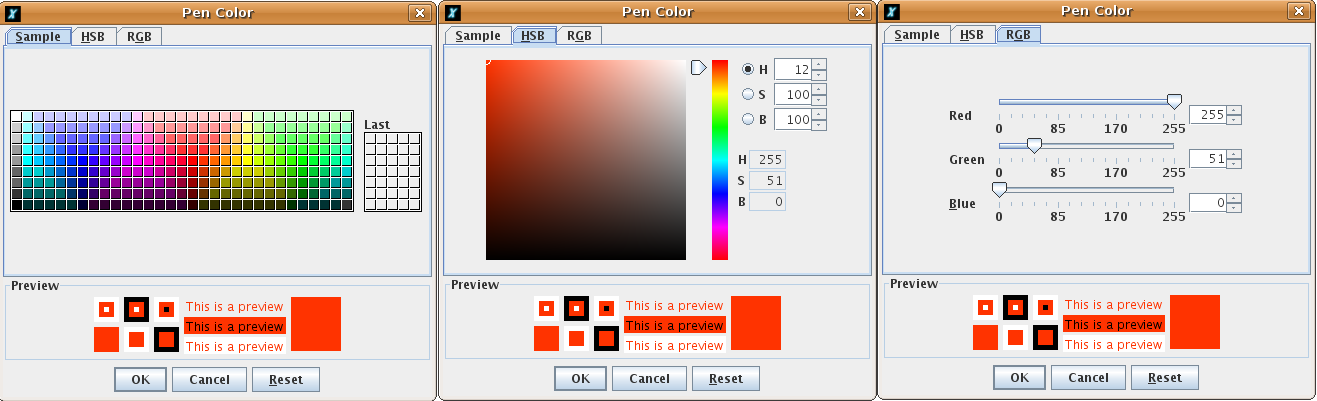
\includegraphics[scale=0.3]{pics/interface-CaptureColor.png}
	\end{center}
	\vspace{0.25cm}
	\item \textbf{Strumenti$\to$Colore Sfondo}: imposta il colore dello sfondo dell'area di disegno, anche accessibile tramite la primitiva \texttt{ImpCS}.
	\item \textbf{Strumenti$\to$File di partenza}: permette di definire il percorso ad un file di avvio. Tutte le procedure contenute in questo file .lgo diventeranno quindi ``pseudo-primitive'' nel linguaggio \xlogo. Non possono essere modificate dall'utente. Puoi quindi definire primitive personalizzate.
	\begin{center}
		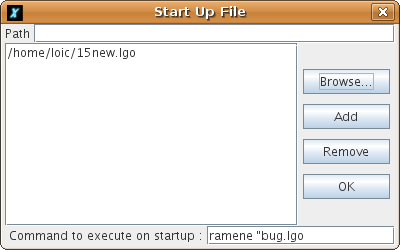
\includegraphics[scale=0.4]{pics/interface-CaptureStart.png}
	\end{center}
	\vspace{0.25cm}
	\item \textbf{Strumenti$\to$Traduttore primitive}: permette di tradurre il codice di \xlogo\ da una lingua all'altra. E' molto utile quando si vuole tradurre un esempio scritto in un'altra lingua.
	\begin{center}
		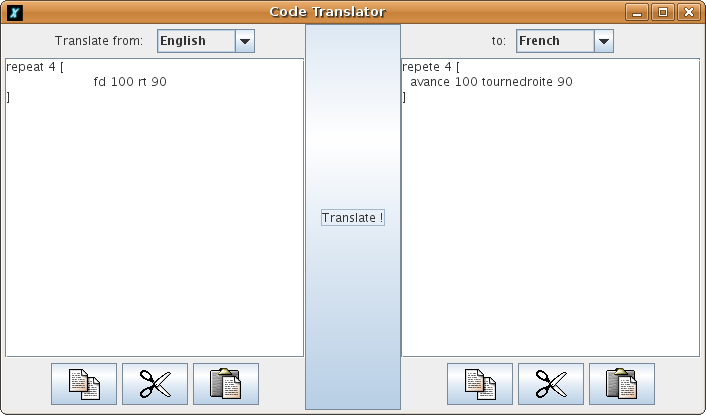
\includegraphics[scale=0.4]{pics/interface-CaptureTranslator.png}
	\end{center}
	\vspace{0.25cm}
	\item \textbf{Strumenti$\to$Gestione procedure}: apre una finestra che permette di cancellare le procedure definite nell'editor. Puoi anche definire l'ordine di comparsa delle procedure nell'editor.
	\begin{center}
		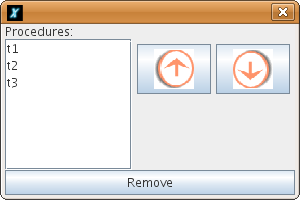
\includegraphics[scale=0.4]{pics/interface-CaptureProcedure.png}
	\end{center}
	\vspace{0.25cm}
	\item \textbf{Strumenti$\to$Preferenze}: apre una finestra che permette di configurare diversi aspetti di \xlogo:
	\begin{itemize}
		\label{general_tab}
		\item \textbf{Tab generale} 
		\begin{itemize}
			\item \textbf{Lingua}: permette di scegliere una diversa lingua, nta che anche le primitive vengono tradotte nella lingua scelta.
			\item \textbf{Aspetto}: permette di impostare l'aspetto di \xlogo tra ``Metal'', ``Nativo  Java'' e ``Motif''.
			\item \textbf{Velocità della tartaruga}: Se preferisci osservare i movimenti della tartaruga puoi rallentarla usando la slitta.
			\end{itemize}. 
			\begin{center}
				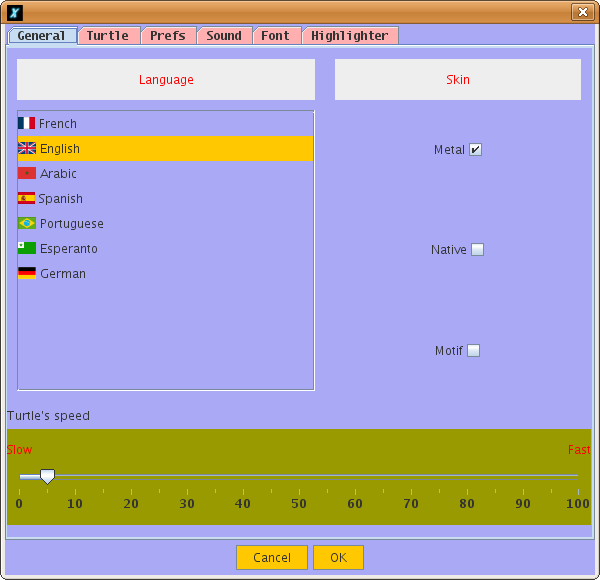
\includegraphics[scale=0.3]{pics/interface-CapturePref1.png}
				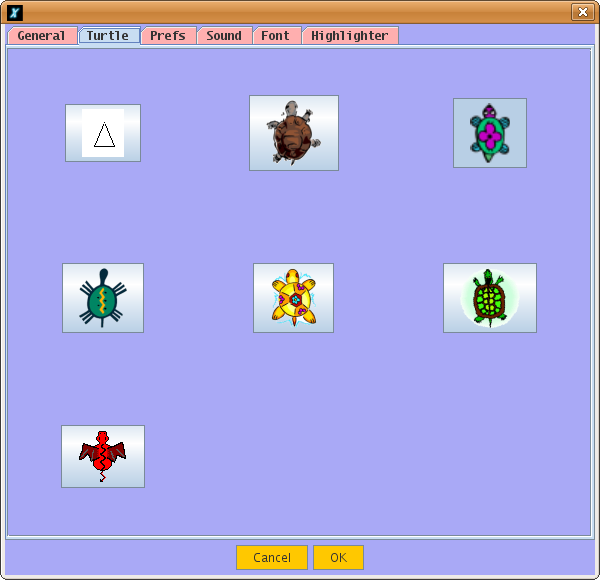
\includegraphics[scale=0.3]{pics/interface-CapturePref2.png}
			\end{center}
			\vspace{0.25cm}
%			\item \textbf{Tab tartaruga}: Puoi scegliere l'immagine della tartaruga che preferisci.
%			\begin{center}
%				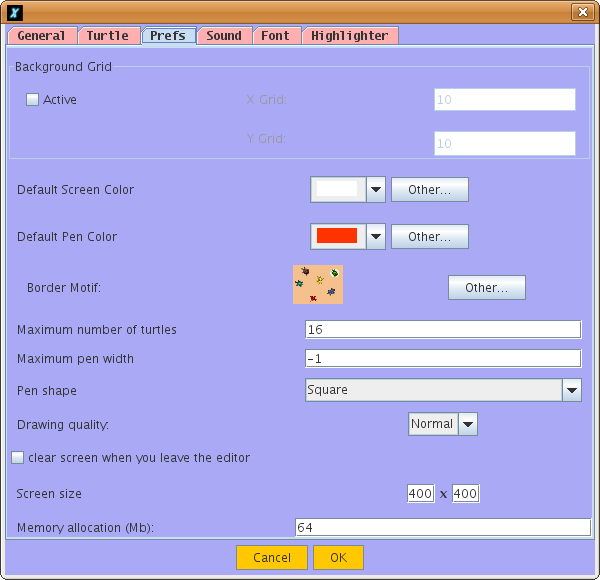
\includegraphics[scale=0.4]{pics/interface-CapturePref3.png}
%			\end{center}
			\item \textbf{Tab opzioni}: Vi sono molte opzioni:
			\begin{itemize}
				\item \textbf{Griglia di sfondo}: Puoi scegliere di disegnare una griglia sullo sfondo dell'area di disegno. Puoi definire l'ampiezza e l'altezza del quadrato della griglia ed il suo colore.
				\item \textbf{Assi sullo sfondo dello schermo}: Puoi disegnare l'asse orizzontale e/o verticale sullo sfondo dell'area di disegno. Puoi definire la distanza tra due divisioni dell'asse ed il colore dell'asse.
				\item \textbf{Colore dello schermo}: Puoi definire un colore dello schermo preimpostato.
				\item \textbf{Colore della penna}: Puoi definire un colore preimpostato della penna.
				\item \textbf{Motivo del bordo}: Puoi scegliere il tuo motivo per l'area esterna a quella del disegno.
				\begin{center}
					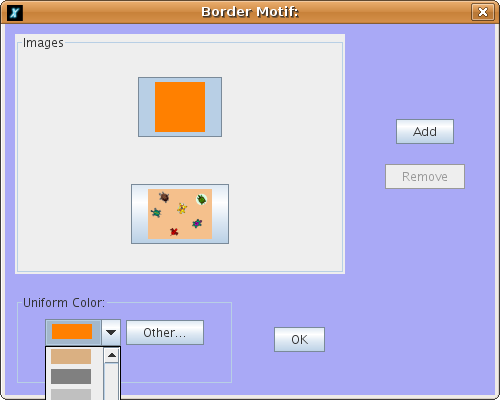
\includegraphics[scale=0.4]{pics/interface-CaptureBorder.png}
				\end{center}
				\item \textbf{Massimo numero di tartarughe}
				\item \textbf{Massima ampiezza della penna}: Puoi scegliere la massima ampiezza della penna permessa (-1 disabilita un limite massimo).
				\item \textbf{Forma della punta della penna}
				\item \textbf{Qualità della traccia da disegno}: Puoi scegliere l'accuratezza della traccia del disegno. In alta qualità gli angoli saranno arrotondati ma la velocità di disegno diminuisce.
				\item \textbf{Pulisci lo schermo quando si chiude l'editor}: alla chiusura dell'editor l'area di disegno viene ripulita o meno.
				\item \textbf{Cancella le variabili quando chiudi l'editor}: alla chiusura dell'editor tutte le variabili vengono cancellate.
				\item \textbf{Dimensione dell'area di disegno}: dimensioni in pixel. Attenzione, aree di disegno più grandi richiedono maggiore memoria.
				\item \textbf{Memoria allocata a XLogo (MB)}: Aree di disegno grandi o programmi ricorsivi hanno bisogno di maggiore memoria di quella predefinita. La modifica di questo parametro richiede di riavviare \xlogo. \textcolor{red}{Attenzione}, non aumentare troppo questo parametro poiché potrebbe rallentare considerevolmente il computer.
				\item \textbf{Numero porta TCP}: Puoi modificare la porta preimpostata TCP per le comunicazioni di rete (cfr. pagina \pageref{network})
			\end{itemize}
			\begin{center}
				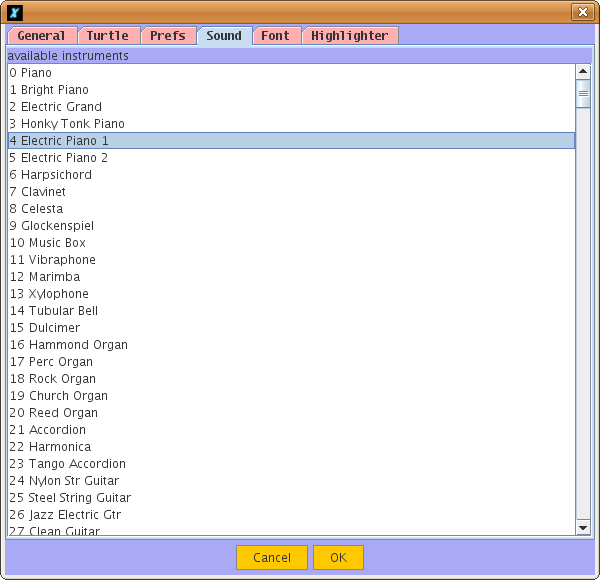
\includegraphics[scale=0.4]{pics/interface-CapturePref4.png}
			\end{center}
			\vspace{0.25cm}
			\item \textbf{Tab Suono}: Puoi scegliere lo strumento musicale per l'interfaccia MIDI. Se l'elenco degli strumenti è vuoto dai uno sguardo alla sezione FAQ del manuale alla fine del manuale. Questa funzione può anche essere acceduta dalla primitiva \texttt{ImpostaStrumento}.
			\begin{center}
				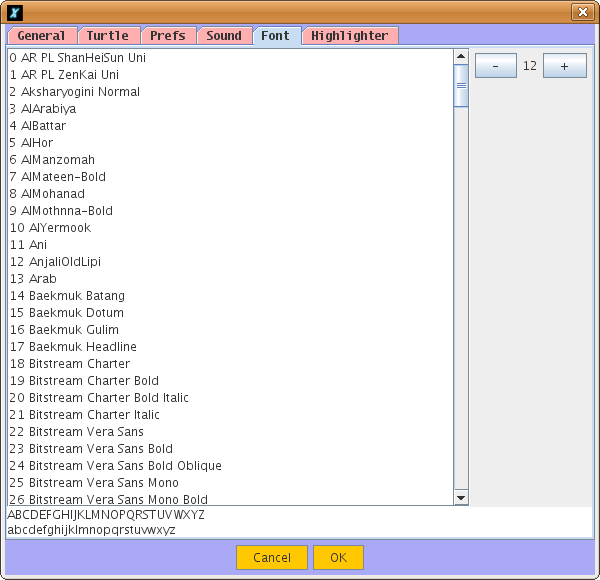
\includegraphics[scale=0.4]{pics/interface-CapturePref5.png}
			\end{center}
			\vspace{0.25cm}
			\item \textbf{Tab Font}: Puoi scegliere il font per l'interfaccia.
			\begin{center}
				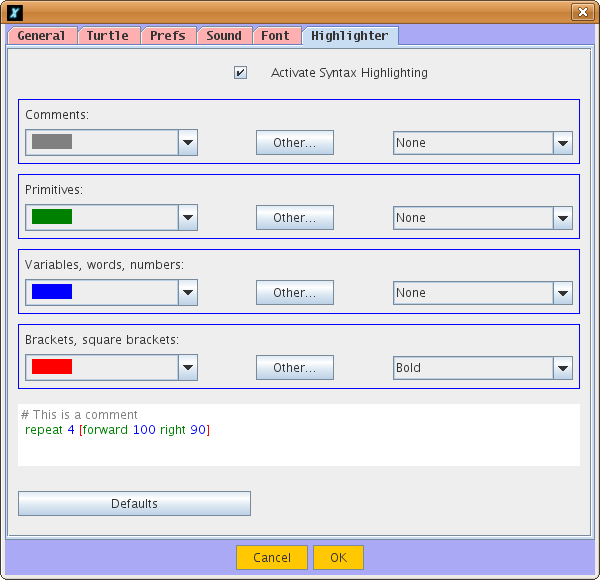
\includegraphics[scale=0.4]{pics/interface-CapturePref6.png}
			\end{center}
			\vspace{0.25cm}
			\item \textbf{Tab Colorazione}: Puoi scegliere di attivare la colorazione sintattica e definire i colori che preferisci.
		\end{itemize}
	\end{itemize}
	\section{Menu ``Aiuto''}
	\begin{itemize}
		\item \textbf{Aiuto$\to$Manuale on-line}: Visualizza il manuale di riferimento per \xlogo, accessibile su Internet.
		\vspace{0.25cm}
		\item \textbf{Aiuto$\to$Licenze}: visualizza la licenza GPL sotto la quale viene distribuito \xlogo.
		\begin{center}
			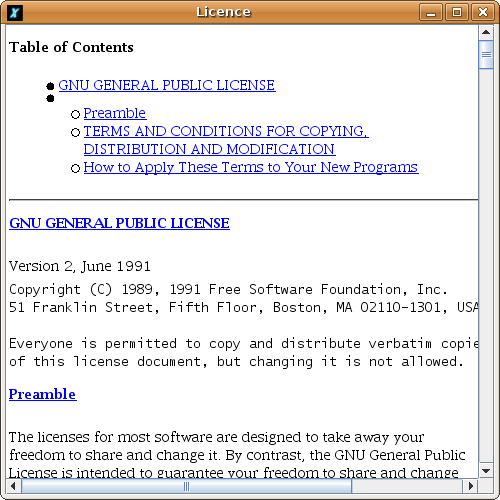
\includegraphics[scale=0.4]{pics/interface-CaptureLicence.png}
		\end{center}
		\vspace{0.25cm}
		\item \textbf{Aiuto$\to$Traduzione della licenza}: visualizza una traduzione della licenza, anche se non ha carattere di ufficialità.
		\item \textbf{Aiuto$\to$Traduci \xlogo}: questa finestra di dialogo permette di consultare, modificare, completare le traduzioni di \xlogo di tutte le lingue (primitive e messaggi).
		\begin{center}
			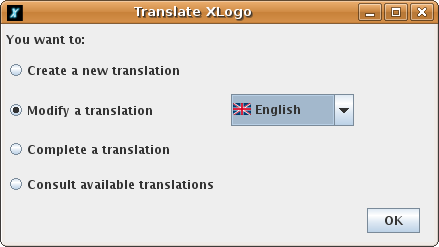
\includegraphics[scale=0.4]{pics/interface-CaptureXLogoTranslate1.png}
			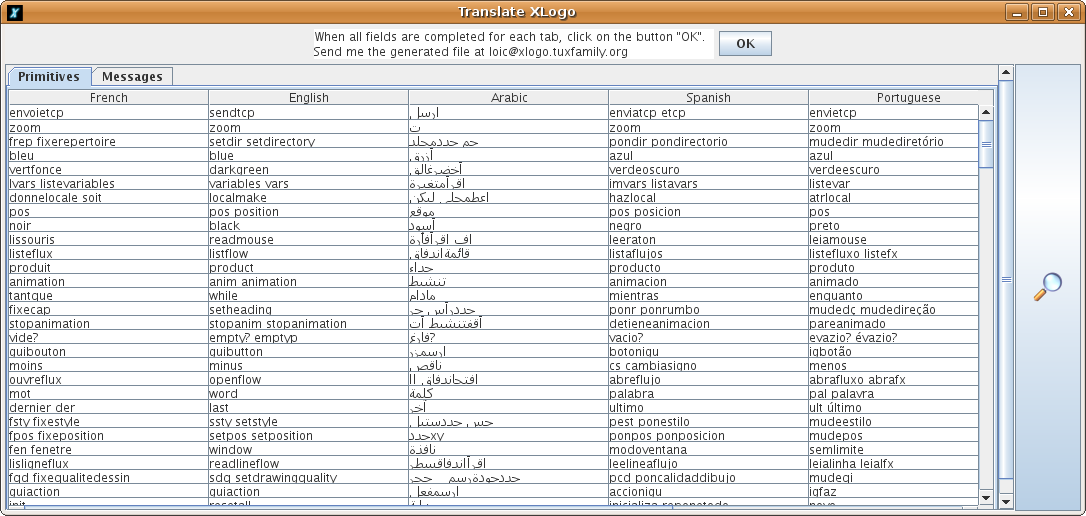
\includegraphics[scale=0.4]{pics/interface-CaptureXLogoTranslate2.png}
		\end{center}
		\vspace{0.25cm}
		Altrimenti puoi creare una traduzione per una nuova lingua. In tutti i casi mandami il file generato a \texttt{loic@xlogo.tuxfamily.org}
		\item \textbf{Menu -- > Informazioni su \xlogo}: la classica finestra e xlogo.tuxfamily.org per i tuoi segnalibri !! o:) 
		\begin{center}
			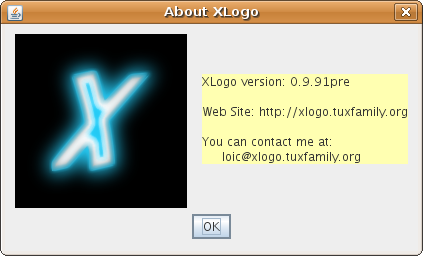
\includegraphics[scale=0.6]{pics/interface-CaptureAbout.png}
		\end{center}
		\vspace{0.25cm}
	\end{itemize}

\chapter{Convenzioni adottate da \xlogo}

Questo capitolo espone alcuni punti chiave circa il linguaggio LOGO e circa \xlogo\ in modo specifico.


\section{I comandi e loro elaborazione}

Il linguaggio LOGO permette di invocare alcuni eventi tramite comandi interni. Questi comandi sono chiamati \textit{primitive}. Ciascuna primitiva può accettare uno o più parametri che vengono chiamati \textit{argomenti}. Per esempio, la primitiva \texttt{PulisciSchermo} non accetta alcun argomento mentre la primitiva \texttt{Somma} accetta due argomenti.\\
\texttt{Stampa Somma 2 3} restituirà 5.\\
\\
Gli argomenti LOGO sono di tre tipi:

\begin{itemize}
	\item \textbf{Numeri}: alcune primitive si aspettano un numero come argomenti: \texttt{Avanti 100} ne è un esempio. 
	\item \textbf{Parole}: le parole sono contrassegnate dai doppi apici (\textquotedbl ) all'inizio del nome della parola stessa. Un esempio di una primitiva che accetta una parola come argomento è \texttt{Stampa}. 
	\begin{center}
		\texttt{Stampa \textquotedbl ciao}
	\end{center}
	Questo comando visualizza \texttt{ciao}. Se viene dimenticato il carattere \textquotedbl\ l'interprete logo restituirà un messaggio di errore. Per l'interprete LOGO \texttt{ciao} non rappresenta niente poiché non è un numero, una parola, un elenco o una procedura già definita.
	\item \textbf{Elenchi}: gli elenchi sono definiti entro parentesi quadre.
\end{itemize}
\textbf{Nota}: i Numeri sono trattati a volte come valori numerici (per esempio \texttt{Avanti 100}), altre volte come parole (per esempio \texttt{Stampa Primo 12} scrive \texttt{1}). \\

\subsection{Le primitive generali}

Molte primitive possiedono una forma generale ossia possono essere usate con un numero di argomenti indefinito. Queste primitive sono:
\begin{center}
	\begin{tabular}{cccc}
		\texttt{Stampa} & \texttt{Somma}&\texttt{Prodotto} &\texttt{o}\\
		\hline
		\texttt{e}&\texttt{Elenco}&\texttt{Frase}& \texttt{Parola}\\
	\end{tabular} 
\end{center}
Per notificare l'interprete LOGO che queste primitive saranno usate nella loro forma generale occorre inscrivere il comando fra parentesi tonde, come nell'esempio seguente:
\begin{lstlisting}
Stampa (Somma 1 2 3 4 5)
# 15

Stampa (Elenco [a b] 1 [c d])
# [a b] 1 [c d] 

Se (e 1=1 2=2 8=5+3) [Avanti 100 RuotaDestra 90]
\end{lstlisting}

\section{Le procedure e le variabili}

Oltre alle primitive è possibile definire comandi personalizzati. Questi comandi sono chiamati \textit{procedure}. Le procedure sono definite mediante le primitive \texttt{Per \textellipsis Fine}. Il blocco di comandi che la procedura eseguirà viene posto all'interno delle due precedenti primitive. Esse possono essere create utilizzando l'editor interno di \xlogo. Ecco un breve esempio:
\begin{lstlisting}
Per quadrato
	Ripeti 4 [Avanti 100 RuotaDestra 90]
Fine
\end{lstlisting}

Come le primitive anche le procedure possono trarre vantaggio degli argomenti. Per passare argomenti alle procedure si utilizzano le variabili. Una variabile è una parola alla quale si può associare (assegnare in termini informatici) un valore. Le variabili sono quindi una sorta di contenitori che possono essere riempiti di valori a nostro piacimento. Ecco un semplice esempio:
\begin{lstlisting}
Per totale :a :b
	Stampa Somma :a :b
Fine
\end{lstlisting} 

Invocando \texttt{totale 2 3} otterremo 5 come risultato.


\section{Il carattere speciale \textbackslash}
Il carattere speciale  \textbackslash \ (barra rovesciata) permette la creazione di parole contenenti simboli vuoti o di particolare significato come l'andare a capo. Se \textbackslash n è usato la frase salta alla linea successiva e \textbackslash\textvisiblespace\ seguito da uno spazio permette di inserire uno spazio in una parola. Per esempio:
\begin{lstlisting}
	Stampa "xlogo\ xlogo
	# xlogo xlogo
	Stampa "xlogo\nxlogo
	# xlogo
	# xlogo
\end{lstlisting}

Per inserire la barra rovesciata in una parola occorre scrivere \textbackslash\textbackslash.\\
Allo stesso modo, per includere quei caratteri a cui \xlogo\ assegna particolari significati ( ( ) [ ] \# ) in una parola occorre prefissarli con la barra rovesciata.  \\
\textbf{Tutti i simboli preceduti da \textbackslash \ sono ignorati. Questo è particolarmente importante nello scrivere i nomi dei file.}. Per esempio per impostare il percorso attuale a \texttt{c:\textbackslash Miei Documenti}:
\begin{lstlisting}
	ImpDir "c:\\Miei\ Documenti.
\end{lstlisting}

Da notare l'uso di \textbackslash\textvisiblespace \ per notificare all'interprete LOGO dell'esistenza dello spazio fra Miei e Documenti. Se si omette la doppia barra rovesciata il percorso diventa  \texttt{c:Miei Documenti} e l'interprete restituirà un messaggio di errore circa l'inesistenza di tale percorso.


\section{Maiuscole e minuscole}

\xlogo\ non fa differenza tra maiuscole e minuscole nei nomi delle procedure e delle primitive. Quindi la procedura \texttt{quadrato} definita precedentemente può essere invocata come \texttt{QUADRATO}, \texttt{Quadrato}, \texttt{qUadrato} e così via, l'interprete LOGO la eseguirà in ogni caso. Al contrario \xlogo\ differenzia le maiuscole dalle minuscole nel caso degli elenchi e delle parole, per esempio:
\begin{lstlisting}
Stampa "Ciao
# Ciao (la maiuscola iniziale viene conservata)
\end{lstlisting}


\section{Gli operatori e la sintassi}

Ci sono due modi per scrivere taluni comandi. Per esempio per sommare 4 e 7 si può usare la primitiva \texttt{Somma} che richiede due argomenti: \texttt{Somma 4 7}, o si può usare l'operatore ``+'': \texttt{4+7}. Entrambi i modi hanno il medesimo effetto. La seguente tabella illustra la relazione tra operatori e primitive:
\begin{center}
	\begin{tabular}{|c|c|c|c|}
		\hline 
		\texttt{Somma}&		\texttt{Differenza}&		\texttt{Prodotto}&		\texttt{Quoziente}\\
		\hline
		+ &		- &		{*} &		/ \\
		\hline
		\texttt{o}&		\texttt{e}&		\texttt{uguale?}&\\
		\hline
		| (ALT GR+6) &		\&&		=&\\
		\hline
	\end{tabular}
\end{center}
\vspace{0.25cm}
Ci sono due altri operatori che non sono associati ad alcuna primitiva:
\begin{itemize}
	\item l'operatore ``Minore o uguale'': \texttt{<=}
	\item l'operatore ``Maggiore o uguale'': \texttt{>=}
\end{itemize}

Nota: I due operatori | e \& sono specifici di \xlogo. Non esistono nelle versioni tradizionali di LOGO. Qualche esempio di impiego:
\begin{lstlisting}
Stampa 3+4=7-1 			# falso
Stampa 3=4 | 7<=49/7	# vero
Stampa 3=4 & 7=49/7		# falso
\end{lstlisting}

\chapter{Découvrir les primitives de base}
{ }\hfill\textbf{Niveau:} débutant\\ \\
\noindent
Pour déplacer la tortue sur l'écran, on utilise des commandes prédéfinies appelées \og primitives\fg. Dans ce chapitre, nous allons découvrir certaines primitives de base permettant de piloter la tortue.
\section{Primitives nouvelles utilisées:}
\noindent \begin{enumerate}
\item  \texttt{av nombre}\hspace {4cm } \textcolor{red}{ \texttt{av 50}}\\
Fait avancer la tortue du nombre de pas de tortues indiqué.
\item  \texttt{re nombre}\hspace {4cm } \textcolor{red}{ \texttt{re 100}}\\
Fait reculer la tortue du nombre de pas de tortues indiqué.
\item  \texttt{td nombre}\hspace {4cm } \textcolor{red}{\texttt{td 90}}\\
La tortue tourne vers la droite de l'angle indiqué.
\item  \texttt{tg nombre}\hspace {4cm } \textcolor{red}{ \texttt{tg 45}}\\
La tortue tourne vers la gauche de l'angle indiqué.
\item  \texttt{ve}\hspace {4cm } \textcolor{red}{ \texttt{ve}}\\
Efface l'écran et initialise la tortue au centre de l'écran.
\item  \texttt{mt}\hspace {4cm } \textcolor{red}{ \texttt{mt}}\\
La tortue est visible à l'écran.
\item  \texttt{ct}\hspace {4cm } \textcolor{red}{ \texttt{ct}}\\
Cache la tortue. Peut permettre de rendre l'affichage plus rapide.
\item  \texttt{lc}\hspace {4cm } \textcolor{red}{ \texttt{lc}}\\
Lève le crayon. La tortue ne laisse plus de trait derrière elle lorsqu'elle se déplace.
\item  \texttt{bc}\hspace {4cm } \textcolor{red}{ \texttt{bc}}\\
Baisse le crayon. La tortue écrit lorsqu'elle se déplace.
\item  \texttt{repete nombre liste}\hspace {4cm } \textcolor{red}{ \texttt{repete 5[av 50 td 45]}}\\
Répète les instructions contenues dans la liste le nombre de fois indiqué.
\end{enumerate}
\section{Dessiner un polygone régulier}
\noindent Ici, nous allons apprendre à tracer un carré, un triangle équilatéral, un pentagone régulier etc
\subsection{Le carré}
\begin{center}
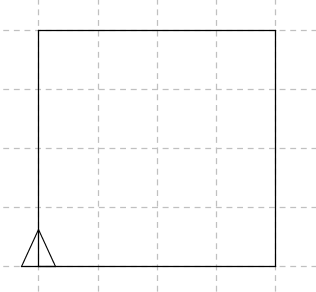
\includegraphics{images/bases-carre.png}
\end{center}
\noindent Un carreau représente 50 pas de tortue. Pour dessiner le carré ci-contre, on va donc taper:
\begin{verbatim}
av 200 td 90 av 200 td 90 av 200 td 90 av 200 td 90
\end{verbatim}
On s'aperçoit ainsi que l'on répète $4$ fois la même instruction d'où une syntaxe plus rapide:
\begin{verbatim}
repete 4[av 200 td 90]
\end{verbatim}
\subsection{Le triangle équilatéral}
\begin{center}
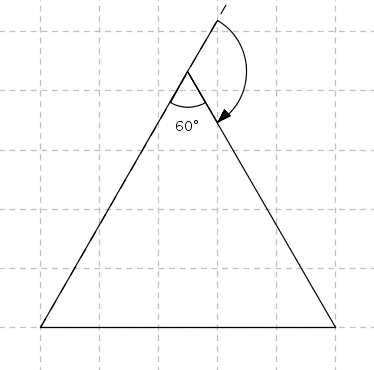
\includegraphics{images/bases-triangle.png}
\end{center}
\noindent Ici, un carreau représente 30 pas de tortues. Nous allons voir ici comment tracer ce triangle équilatéral de 150 pas de tortue de côté.\\ \\
La commande ressemblera à quelque chose du style: 
\begin{verbatim}
repete 3[av 150 td ....]
\end{verbatim}
Reste à déterminer le bon angle. Dans un triangle équilatéral, les angles valent tous 60 degrés. Comme la tortue doit tourner à l'extérieur du triangle. L'angle vaudra 180-60=120 degrés. La commande est donc:
\begin{verbatim}
repete 3[av 150 td 120]
\end{verbatim}
\subsection{L'hexagone}
\begin{center}
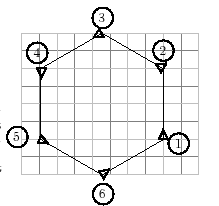
\includegraphics{images/bases-hexagone.png}
\end{center}
\noindent Ici, un carreau représente 20 pas de tortues.\\
\begin{verbatim}
repete 6[av 80 td ....]
\end{verbatim}
On s'aperçoit que lors de son déplacement, la tortue effectue en fait un tour complet sur elle même. (Elle part orientée vers le haut puis revient dans cette position). Cette rotation de 360 degrés s'effectue en 6 étapes.\\
 Par conséquent, à chaque fois, elle tourne de $\dfrac{360}{6}=60$\degre. \\ \\
La commande est donc: \texttt{repete 6[av 80 td 60]}

\subsection{Tracer un polygone régulier en général}
\noindent En fait, en réitérant le petit raisonnement précédent, on s'aperçoit que pour tracer un polygone à $n$ côtés, l'angle s'obtiendra en divisant 360 par $n$. Par exemple:\begin{itemize}
\item Pour tracer un pentagone régulier de côté 100:
\begin{verbatim}
repete 5[av 100 td 72]    (360:5=72)
\end{verbatim}
\item Pour tracer un ennagone régulier (9 côtés) de côté 20:
\begin{verbatim}
repete 9[av 20 td 40]    (360:9=40)
\end{verbatim}
\item Pour tracer un euh... 360-gone régulier de côté 2: (ça ressemble fortement à un cercle, ça!)
\begin{verbatim}
repete 360[av 2 td 1]  
\end{verbatim}
\item Pour tracer un heptagone de côté 120:
\begin{verbatim}
repete 7[av 120 td 360/7]
\end{verbatim}
\end{itemize}

\section{Enregistrer une procédure}
\noindent Pour éviter d'avoir à retaper à chaque fois les instructions pour
dessiner un carré, un triangle ... on peut définir des instructions personnelles appelées \og procédures \fg. Une procédure commence par le mot-clé \texttt{pour} et se termine par le mot-clé \texttt{fin}. On ouvre l'éditeur, on tape par exemple

\begin{verbatim}
pour carre
repete 4[av 100 td 90]
fin
\end{verbatim}
puis on ferme l'éditeur en enregistrant les modifications en cliquant sur le bouton tortue.  Maintenant à chaque fois que l'on tape \texttt{carre}, un carré apparaît à l'écran!

\section{Exercice ...}
\noindent
Un petit carreau représente 10 pas de tortue.\\
Essayer de réaliser le dessin ci-dessous en définissant huit procédures:
\begin{itemize}
\item Une procédure \og \texttt{carre} \fg{} qui tracera le carre de base
de la maison.
\item Une procédure \og \texttt{tri} \fg{} qui tracera le triangle équilatéral
représentant le toit de la maison.
\item Une procédure \og \texttt{porte} \fg{} qui tracera le rectangle
représentant la porte.
\item Une procédure \og \texttt{che} \fg{} qui tracera la cheminée
\item Une procédure \og \texttt{dep1} \fg{} qui permettra à la tortue
de se déplacer de la position A à la position B.
\item Une procédure \og \texttt{dep2} \fg{} qui permettra à la tortue
de se déplacer de la position B à la position C.
\item Une procédure \og \texttt{dep3} \fg{} qui permettra à la tortue
de se déplacer de la position C à la position D. (Attention, il faudra
peut-être lever le crayon de la tortue...)
\item Une procédure \og \texttt{ma} \fg{} qui permettra de tracer la maison
en entier en s'aidant de toutes les autres procédures.
\end{itemize}
\label{maison}
\begin{center}
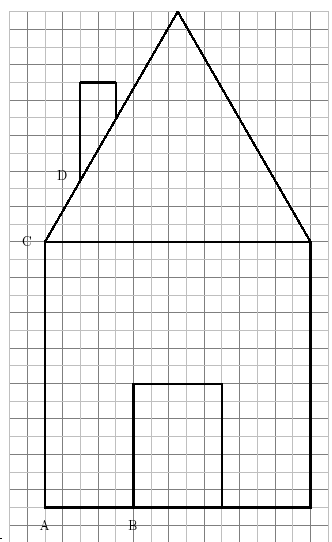
\includegraphics[scale=0.6]{images/bases-maison.png}
\end{center}
\chapter{Uzi koordinatojn}
\label{koordinatoj}

{ }\hfill\textbf{Nivelo:} komencanto
\section{Prezentado}
\noindent En tiu ^ci ^capitro, ni malkovros la primitivon
\texttt{situon\_provizu}.  La desegnareo havas dratreton kies origino
estas lokita je la centro de la ekrano.  Oni povas atingi ^ciun
punkton de la desegnejo per helpo de ^giaj koordinatoj.

\texttt{sitp listo}\hspace {4cm } \textcolor{red}{ \texttt{sitp [100 -250]}}\\
Movas la testudon al la punkto kies koordinatojn difinas la listo.\\ \\
\\ Malgranda uzekzemplo:\\
\texttt{ev sitp [200 100] sitp [50 -150] sitp [-100 -150]}
\begin{center}
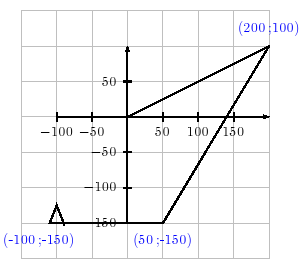
\includegraphics[scale=0.7]{bildoj/fpos-coord.png}
\end{center}
\vspace{1cm}
\section{Ekzerco:}
\noindent
Realigu tiun figuron nur uzante la primitivojn: \texttt{sitp}, \texttt{ev}, \texttt{l}, \texttt{ml}.\\
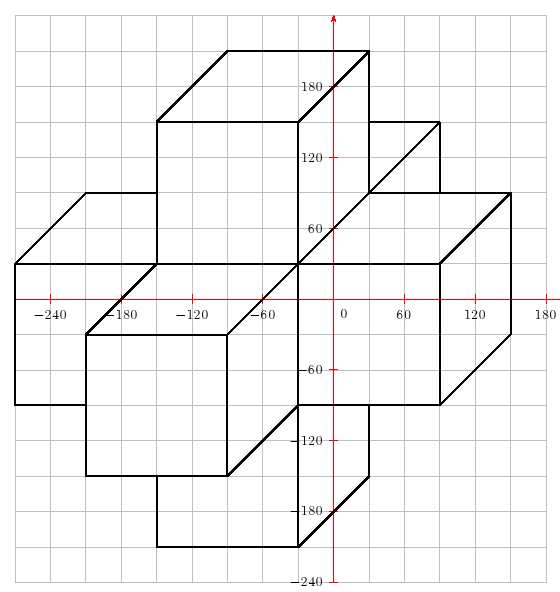
\includegraphics[scale=0.7]{bildoj/fpos-cube.png}

\chapter{Les variables}
{ }\hfill\textbf{Niveau:} débutant\\ \\
\noindent \noindent Parfois, on souhaite tracer une figure à différentes échelles. Par exemple, si on souhaite dessiner un carré de côté 100, un carré de côté 200 et un carré de côté 50, actuellement on définirait trois procédures différentes correspondant à chacun de ces carrés. 
\begin{verbatim}
pour carre1
repete 4 [av 100 td 90]
fin
pour carre2
repete 4 [av 200 td 90]
fin
pour carre3
repete 4 [av 50 td 90]
fin
\end{verbatim}
On s'aperçoit immédiatement qu'il serait plus simple de définir une seule procédure à laquelle on préciserait juste la longueur du côté à tracer. Par exemple, \texttt{carre 200} tracerait le carré de côté 200, \texttt{carre 100} tracerait le carré de côté 100 etc. C'est précisément ce que vont permettre de réaliser les variables.
\section{Exemples d'utilisation}
\noindent Pour tracer un carré de côté 100, on utilise:
\begin{verbatim}
pour carre
repete 4[av 100 td 90]
fin
\end{verbatim}
Nous allons modifier cette procédure afin qu'elle reçoive un paramètre (on dit également \og argument \fg) indiquant la longueur du côté à tracer. \\
Un nom de variable est toujours précédée du symbole \og : \fg. Lorsqu'on veux indiquer que la procédure \texttt{carre} dépend de la variable \texttt{:c}, on rajoute \texttt{:c} à la fin de la ligne de défnition. \\
Par conséquent, ensuite, on avancera non plus de 100 pas de tortue mais de \texttt{:c} pas de tortues. La procédure devient alors:
\begin{verbatim}

pour carre :c
repete 4[av :c td 90]
fin
\end{verbatim}
Ainsi, en tapant: \texttt{carre 100 carre 50 carre 30 carre 20 carre 10}\\
 \begin{center}
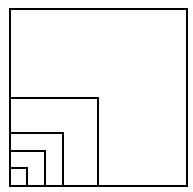
\includegraphics[scale=0.5]{images/variables-carres.png}
\end{center}
 \vspace{1cm}
 \section{Tracer un rectangle de longueur et largeur déterminée}
 \noindent On définit ici une procedure nommée \texttt{rec} qui dépend de deux variables représentant les deux dimensions du rectangles. \texttt{rec 200 100} trace ainsi un rectangle de hauteur 200 et largeur 100.
 \begin{verbatim}
pour rec :lo :la
repete 2[av :lo td 90 av :la td 90]
fin
\end{verbatim} 
Faites des essais: 
\begin{verbatim}
rec 200 100 rec 100 300 rec 50 150 rec 1 20 rec 100 2 
\end{verbatim}
Bien sûr, si vous ne donnez qu'un argument à la procédure \texttt{rec}, l'interpréteur vous signalera par un message d'erreur que la procédure attend un autre argument.
\section{Tracer une forme à des tailles diverses}
\noindent
Nous avons vu comment tracer un carré, un rectangle à des tailles différentes. Nous allons reprendre l'exemple de la maison p. \pageref{maison} et voir comment modifier le code pour tracer la maison à l'échelle souhaitée.\\ \\
L'objectif est de passer un argument à la procédure \texttt{ma} pour que selon le paramètre, la maison soit plus ou moins grande. Nous souhaitons que \texttt{ma 1} trace la maison en taille réelle.\\
\texttt{ma 0,5} tracera une maison à l'échelle 0,5. \\
\texttt{ma 2} tracera une maison aux dimensions deux fois plus grandes etc \\ \\
La notion de proportionnalité est bien sûr sous-jacente. En vraie grandeur, la procédure \texttt{carre} était la suivante:
\begin{verbatim}
pour carre 
repete 4[av 150 td 90]
fin
\end{verbatim}
Toutes les dimensions originales de la maison sont multipliées par l'échelle. La procédure \texttt{carre} devient: 
\begin{verbatim}
pour carre :c
repete 4[av 150*:c td 90]
fin
\end{verbatim}
Ainsi quand on tapera \texttt{carre 2}, le carré aura pour côté $150\times2=300$. les proportions sont bien respectées! En fait, on s'aperçoit qu'il va juste falloir reprendre toutes les procédures et changer les longueurs de déplacement de la manière suivante: \\
\texttt{av 70} devient \texttt{av 70*:c} \\ 
\texttt{av 45} devient \texttt{av 45*:c} \\
etc\\ \\
\begin{verbatim}
pour carre :c
repete 4[av 150*:c  td 90]
fin

pour tri :c
repete 3[av 150*:c td 120]
fin

pour porte :c
repete 2[av 70*:c td 90 av 50*:c td 90]
fin

pour che :c
av 55*:c td 90 av 20*:c td 90 av 20*:c
fin

pour dep1 :c
td 90 av 50*:c tg 90
fin

pour dep2 :c
tg 90 av 50*:c td 90 av 150*:c td 30
fin

pour dep3 :c
lc td 60 av 20*:c tg 90 av 35*:c bc
fin

pour ma :c
carre :c dep1 :c porte :c dep2 :c tri :c dep3 :c che :c
fin
\end{verbatim}
\section{Exercice:}
\noindent Réaliser les dessins suivants avec des variables de telle sorte que l'on puisse les obtenir à des tailles diverses.\\ \\ \\
\begin{center}
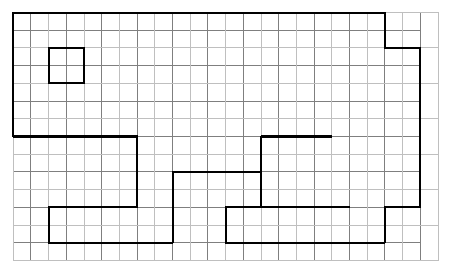
\includegraphics[scale=0.7]{images/variables-grenouille.png}
\end{center}
\begin{center}
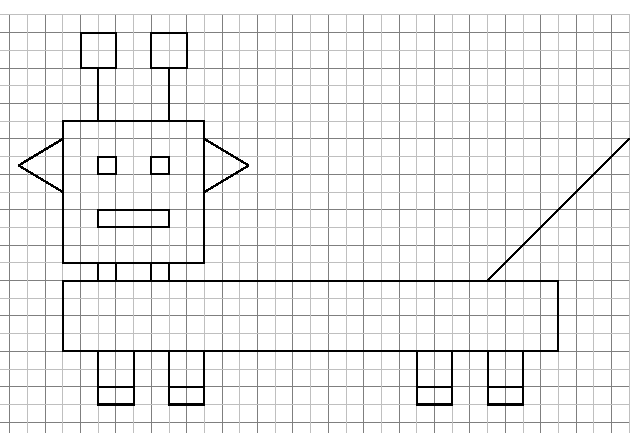
\includegraphics[scale=0.75]{images/variables-robot.png}
\end{center}

\chapter{La récursivité}
{ }\hfill\textbf{Niveau:} moyen\\ \\
\noindent Le langage Logo utilise très souvent une technique de programmation appelée la récursivité. Dans ce chapitre, nous découvrirons tout d'abord cette notion sur des exemples simples pour ensuite approfondir avec notamment le tracé d'une fractale appelée  le flocon de Van Koch. Pour commencer, petite explication:
\begin{center}
\textbf{Une procédure est récursive si elle s'appelle elle-même.}                                                                 \end{center}
\section{Avec la zone de dessin.}
\subsection{ Premier exemple:}
\begin{verbatim}
pour ex1
td 1
ex1
fin  
\end{verbatim}
Cette procédure est récursive puisque la procédure \texttt{ex1} est appelée à la dernière ligne. A l'exécution, on constate que la tortue ne cesse de tourner sur elle-même. Pour interrompre le programme, on est obligé de se servir du bouton STOP.
\subsection{Deuxième exemple:}
\noindent Tout d'abord, voici trois nouvelles primitives:
\begin{itemize}
\item [$\bullet$] \texttt{attends nombre}\hspace {4cm } \textcolor{red}{ \texttt{attends 60}}\\
Bloque le programme pendant le nombre de 60$^{\textrm{ième}}$ de secondes indiqué. \\
Par exemple, \texttt{attends 120} bloquera le programme pendant deux secondes.
\item [$\bullet$] \texttt{gomme}\hspace {4cm } \textcolor{red}{{gomme}}\\
Lorsque la tortue se déplace, elle efface tout au lieu de laisser un trait derrière elle.
\item [$\bullet$] \texttt{dessine,de}\hspace {4cm } \textcolor{red}{{dessine}}\\
Repasse en mode dessin classique: la tortue laisse un trait derrière elle en se déplaçant.
\end{itemize}
\noindent
\begin{verbatim}
pour ex2
av 200 gomme attends 60
re 200 dessine td 6
ex2
fin
\end{verbatim}
Il ne reste plus qu'à lancer ce programme. A chaque seconde le même motif recommence et le programme simule ainsi une trotteuse!
\section{Avec la zone de texte}
\subsection{Un premier exemple:}
\noindent La primitive \texttt{ecris, ec} permet d'afficher un texte dans la zone de texte. elle attend pour argument soit une liste soit un mot. Ex: \texttt{ec "bonjour} \texttt{ec [J'écris ce que je veux]} (Ne pas oublier la quote " lorsqu'on veut juste écrire un mot.)
\begin{verbatim}
pour ex3 :n
ecris :n
ex3 :n+1
fin
\end{verbatim}
Lancer la commande \texttt{ex3 0} puis interrompre avec le bouton STOP\\
Faites les changements nécessaires dans ce programme pour que les chiffres apparaissent de deux en deux.\\
\\
Je veux à présent afficher tous les chiffres supérieur à 100 qui sont dans la table de cinq. Il suffit alors de modifier le programme ainsi:
\begin{verbatim}
pour ex3 :n
ecris :n
ex3 :n+5
fin
\end{verbatim}
 et de lancer: \texttt{ex3 100}
\subsection{Réaliser un test de sortie}
\noindent Taper les commandes suivantes:\\
\texttt{si 2+1=3 [ecris [ceci est vrai]]} \\
\texttt{si 2+1=4 [ecris [ceci est vrai]][ecris [le calcul est faux]]} \\
\texttt{si 2+5=7 [ec "vrai][ec "faux]}\\
\\
Si vous n'avez toujours pas compris la syntaxe de la primtive \texttt{si}, reportez-vous au manuel de référence de \xlogo.
\begin{verbatim}
pour ex3 :n
si :n=100 [stop]
ecris :n
ex3 :n+1
fin
\end{verbatim}
Lancer la commande \texttt{ex3 0}\\
Faites les changements nécessaires dans ce programme pour faire apparaître les chiffres compris entre et 55 et 350 qui sont dans la table de 11.\\
\section{Un exemple de fractale: le flocon de Van Koch}
\noindent Grâce à la récursivité, il est très facile de générer en \logo\ des objets que l'on appelle  en mathématiques des fractales. \\ \\
Voici les premières étapes permettant de créer la ligne brisée de Van Koch. 
\begin{center}
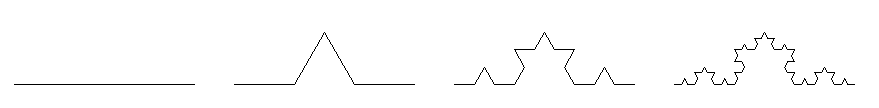
\includegraphics[width=\textwidth]{images/koch0123.png}
\end{center}
Entre chaque étape:
\begin{enumerate}
 \item chacun des segments est partagé en trois parties égales.
 \item on trace un triangle équilatéral sur le deuxième segment.
 \item on efface ce deuxième segment.
\end{enumerate}
\textbf{Ce qu'il faut remarquer:}  Prenons le cas de la deuxième étape, on constate que cette ligne est formée de quatre motifs correspondant à l'étape précédente et dont la taille est divisée par 3. On vient de mettre en évidence la nature récursive de la fractale.\\ \\
Appelons $L_{n,\ell}$ le motif de longueur $\ell$, tracé à l'étape $n$.\\
Pour tracer ce motif voici le procédé:
\begin{enumerate}
 \item On trace $L_{n-1,\ell/3}$
 \item On tourne à gauche de 60 degrés
 \item On trace $L_{n-1,\ell/3}$
 \item On tourne à droite de 120 degrés
 \item On trace $L_{n-1,\ell/3}$
 \item On tourne à gauche de 60 degrés
 \item On trace $L_{n-1,\ell/3}$
\end{enumerate}
En \logo, cela donne tout simplement:
\begin{verbatim}
# :l longueur du motif
# :p étape
pour ligne :l :p
si :p=0 [av :l] [
  ligne :l/3 :p-1 tg 60 ligne :l/3 :p-1 td 120 ligne :l/3 :p-1 tg 60 ligne :l/3 :p-1
]
fin
\end{verbatim}
Si l'on trace un triangle équilatéral composé de trois de ces lignes, on obtient un magnifique flocon de Van Koch
\begin{verbatim}
# :l longueur du côté
pour flocon :l :p
repete 3[ligne :l :p td 120]
fin
\end{verbatim}
Puis en lançant: \texttt{flocon 200 6}
\begin{center}
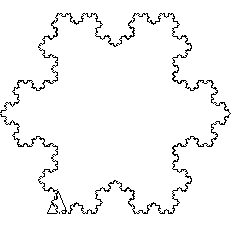
\includegraphics{images/flocon.png}
\end{center}
\section{Recursivite sur les mots}
\noindent Consulter la liste des primitives p.\pageref{liste-prim} afin de comprendre le rôle des primitives \texttt{mot}, \texttt{dernier}, et \texttt{saufdernier}.\\ \\
Voici une procédure récursive qui permet d'inverser l'ordre des lettres d'un mot
\begin{verbatim}
pour inversem :m
si vide? :m [retourne "]  
retourne mot dernier :m inversem saufdernier :m
fin

ecris inversem "abcde
edcba
\end{verbatim}
On dit qu'un mot est un palindrome si on peut le lire dans les deux sens (exemples: radar, laval ...).
\begin{verbatim}
# teste si le mot :m est un palindrome
pour palindrome :m
si  :m=inversem :m [retourne vrai] [retourne faux] 
fin
\end{verbatim}
Et enfin ce joli petit programme (Merci Olivier SC):
\begin{verbatim}
pour palin :n
si palindrome :n [ecris :n stop]
ecris (liste :n "PLUS inversem :n "EGAL somme :n inversem :n)
palin :n + inversem :n 
fin

palin 78
78 PLUS 87 EGAL 165
165 PLUS 561 EGAL 726
726 PLUS 627 EGAL 1353
1353 PLUS 3531 EGAL 4884
4884
\end{verbatim}
\section{Calculer un factorielle}
\label{factorielle}
\noindent On définit factorielle de 5, noté $5!$ par:
 $$5!=5\times4\times3\times2\times1=120$$
De manière générale pour $n$ strictement positif, on remarque que: $n!=n\times(n-1)!$.\\
Cette relation explique la nature récursive de ce programme:
\begin{verbatim}
pour fac :n
si :n=0[ret 1][ret :n*fac :n-1]
fin

ec fac 5
120
ec fac 6
720
\end{verbatim} 
 \section{Une approximation de $\pi$}
\label{approx-pi}
\noindent On peut obtenir une approximation du nombre $\pi$ avec la formule:
$$\pi\approx2^k\sqrt{2-\sqrt{2+\sqrt{2+\ldots\sqrt{2+\sqrt2}}}}$$ où $k$ est le nombre de racines carrées. Plus $k$ devient grand et plus cette expression se rapproche du nombre $\pi$.\\ \\
La formule est constituée de l'expression $2+\sqrt{2+\ldots\sqrt{2+\sqrt2}}$ qui est clairement récursive d'où le programme:
\begin{verbatim}
# k désigne le nombre de racines
pour approxpi :k
tape "Approximation:\  ec (puissance 2 :k) * racine (2- racine (calc :k-2))
ec "-------------------------
tape "Pi:\  ec pi
fin

pour calc :p
si :p=0 [ret 2][ret 2+racine calc :p-1]
fin

approxpi 10
Approximation: 3.141591421568446 
------------------------- 
Pi: 3.141592653589793 
\end{verbatim}
On a obtenu les 5 premières décimales! Si l'on souhaite davantage, il faudra éliminer certaines erreurs de calculs dues aux racines carrées imbriquées. Pour cela nous allons augmenter le nombre de décimales avec la primitive \texttt{fixedecimales}.
\begin{verbatim}
fixedecimales 100
approxpi 100
Approximation: 3.1415926535897932384626433832795028841973393069670160975807684313880468...
------------------------- 
Pi: 3.141592653589793238462643383279502884197169399375105820974944592307816406....
\end{verbatim}
Et on obtient à présent 39 décimales...
\chapter{Create an animation}
{ }\hfill\textbf{Level:} Medium\\ \\
This chapter presents two different themes with the goal of creating animation in \xlogo.
\section{Calculator's numbers}
\begin{center}
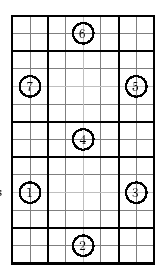
\includegraphics{pics/animation-chiffre.png}
\end{center}
\noindent This theme is based on the fact that every calculator's number could be drawn with the above schema:
\begin{itemize}
\item For example, to draw digit 4, we light rectangles 3,4,5,7.
\item To draw digit 8, we light rectangles 1,2,3,4,5,6,7.
\item To draw digit 3, we light rectangles 2,3,4,5,6.
\end{itemize}

\subsection{Filling a rectangular}
\begin{center}
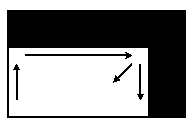
\includegraphics{pics/animation-rectangle.png}
\end{center}
\noindent If we want to draw a filled rectangle with dimensions 100 by 200, a first idea could be to draw a rectangle 100 by 200 then to draw a rectangle 99 by 199, then a rectangle 98 by 198 ... until the rectangle is fully filled.  \\
Let's begin by defining a rectangle with two variables corresponding to width and height
\begin{verbatim}
to rec :h :w
repeat 2[fd :h rt 90 fd :w rt 90]
end
\end{verbatim}
To fill our rectangle, we have to run:\\
\texttt{rec 100 200 rec 99 199 rec 98 198  ..... rec 1 101}\\ \\
Let's define a procedure for this filled rectangle.
\begin{verbatim}
to rectangular :h :w
rec :h :w
rectangular :h-1 :w-1
end
\end{verbatim}
We test \texttt{rectangular 100 200} and we can see there is a problem: The procedure doesn't stop when the rectangle has been filled, it continues infinitely! We must add a breakout test that will detect if width or height is equal to 0. When this condition is realized, we'll ask the program to stop with the primitive \texttt{stop}.
\begin{verbatim}
to rectangular :h :w
if or :h=0 :w=0 [stop]
rec :h :w
rectangular :h-1 :w-1
end
\end{verbatim}
Note: Instead of using the primitive \texttt{or}, it's possible to use the symbol |, the line becomes:
 \begin{center}
\texttt{if :h=0 | :w=0 [stop]}
\end{center}
\subsection{The program}
\noindent We must reuse the precedent filled rectangle:
\begin{verbatim}
to rectangular :h :w
if or :h=0 :w=0 [stop]
rec :h :w
rectangular :h-1 :w-1
end
\end{verbatim}
We suppose that the turtle starts from the bottom left corner. We're going to define a procedure called \texttt{number} depending on 7 arguments \texttt{:a}, \texttt{:b}, \texttt{:c}, \texttt{:d}, \texttt{:e}, \texttt{:f}, \texttt{:g}. When \texttt{:a} is equal to 1, we draw the rectangle 1. If \texttt{:a} is equal to 0, we don't draw this rectangle. Here is the main idea.\\ \\
\textbf{The code}:
\begin{verbatim}
to number :a :b :c :d :e :f :g
# we draw the rectangular 1
if :a=1 [rectangular 160 40]
# we draw the rectangular 2
if :b=1 [rectangular 40 160]
penup right 90 forward 120 left 90 pendown
# we draw the rectangular 3
if :c=1 [rectangular 160 40]
penup forward 120 pendown
# we draw the rectangular 5
if :e=1 [rectangular 160 40]
# we draw the rectangular 4
left 90 penup back 40 pendown
if :d=1 [rectangular 160 40]
# we draw the rectangular 6
right 90 penup forward 120 left 90 pendown
if :f=1 [rectangular 160 40]
# we draw the rectangular 7
penup forward 120 left 90 back 40 pendown 
if :g=1 [rectangular 160 40]
end

\end{verbatim}
\subsection{Creating an animation}
\noindent In this part, we'll define a countdown from 9 to 0.
\begin{verbatim}
to countd
clearscreen hideturtle number 0 1 1 1 1 1 1 wait 60
clearscreen hideturtle number 1 1 1 1 1 1 1 wait 60
clearscreen hideturtle number 0 0 1 0 1 1 0 wait 60
clearscreen hideturtle number 1 1 1 1 0 1 1 wait 60
clearscreen hideturtle number 0 1 1 1 0 1 1 wait 60
clearscreen hideturtle number 0 0 1 1 1 0 1 wait 60
clearscreen hideturtle number 0 1 1 1 1 1 0 wait 60
clearscreen hideturtle number 1 1 0 1 1 1 0 wait 60
clearscreen hideturtle number 0 0 1 0 1 0 0 wait 60
clearscreen hideturtle number 1 1 1 0 1 1 1 wait 60
end
\end{verbatim}
Little problem: There is a flickering effect during each number drawing. To make the animation fluid, we're going to use the three primitives \texttt{animation}, \texttt{stopanimation} and \texttt{repaint}.\\
\begin{itemize}
\item \texttt{animation} enables the mode ``animation''. The turtle stops drawing on the screen but remembers all changes in cache. To display the image, it's necessary to use the primtive \texttt{repaint}.
\item  \texttt{stopanimation} returns to the classic drawing mode.
\end{itemize}
Here is the new code for this procedure:
\begin{verbatim}
to countd
# Enables animation mode
animation
clearscreen hideturtle number 0 1 1 1 1 1 1 repaint wait 60
clearscreen hideturtle number 1 1 1 1 1 1 1 repaint wait 60
clearscreen hideturtle number 0 0 1 0 1 1 0 repaint wait 60
clearscreen hideturtle number 1 1 1 1 0 1 1 repaint wait 60
clearscreen hideturtle number 0 1 1 1 0 1 1 repaint wait 60
clearscreen hideturtle number 0 0 1 1 1 0 1 repaint wait 60
clearscreen hideturtle number 0 1 1 1 1 1 0 repaint wait 60
clearscreen hideturtle number 1 1 0 1 1 1 0 repaint wait 60
clearscreen hideturtle number 0 0 1 0 1 0 0 repaint wait 60
clearscreen hideturtle number 1 1 1 0 1 1 1 repaint wait 60
# back to classic mode
stopanimation
end
\end{verbatim}
\section{Second animation: The growing man}
\begin{center}
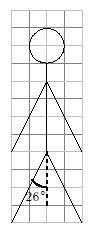
\includegraphics{pics/animation-bonhomme.png}
\end{center}
First, we'll define a procedure \texttt{man} that draws the above schema. We use a variable to reproduce it at different scales 
\begin{verbatim}
to man :c
left 154 forward 44*:c back 44*:c 
left 52 forward 44*:c back 44*:c 
left 154 forward 40*:c
left 154 forward 44*:c back :c*44 
left 52 forward 44*:c back :c*44 
left 154 forward 10*:c
left 90 repeat 180[forward :c/2 right 2] right 90
end
\end{verbatim}
Now, we'll create an animation that will make the man grow. To realize this, we'll draw \texttt{man 0.1}, then \texttt{man 0.2} \texttt{man 0.3} ... until \texttt{man 5}. Between each man, we'll erase the screen. We obtain two different procedures:
\begin{verbatim}
to man :c
left 154 forward 44*:c back 44*:c 
left 52 forward 44*:c back 44*:c 
left 154 forward 40*:c
left 154 forward 44*:c back :c*44 
left 52 forward 44*:c back :c*44 
left 154 forward 10*:c
left 90 repeat 180[forward :c/2 right 2] right 90
if :c=5[stop]
cs ht man :c+0.1
end

to go
cs ht
man 0
end
\end{verbatim}
Finally to make the animation fluid, we'll use animation mode and the primitive \texttt{repaint}.
\begin{verbatim}
to man :c
left 154 forward 44*:c back 44*:c 
left 52 forward 44*:c back 44*:c 
left 154 forward 40*:c
left 154 forward 44*:c back :c*44 
left 52 forward 44*:c back :c*44 
left 154 forward 10*:c
left 90 repeat 180[forward :c/2 right 2] right 90
repaint
if :c=5[stop]
cs ht man :c+0.1
end

to go
cs ht animation
man 0
stopanimation
end
\end{verbatim}
\textbf{Note: } Here, the procedure \texttt{man} is recursive. In aother way, we could use the primitive \texttt{for} to make the variable \texttt{:c} from 0.1 to 5. Here is the program:
\begin{verbatim}
to man :c
cs left 154 forward 44*:c back 44*:c 
left 52 forward 44*:c back 44*:c 
left 154 forward 40*:c
left 154 forward 44*:c back :c*44 
left 52 forward 44*:c back :c*44 
left 154 forward 10*:c
left 90 repeat 180[forward :c/2 right 2] right 90
repaint
end

to go
ht animation
for [c 0 5 0.1][man :c]
stopanimation
end
\end{verbatim}
\chapter{Interact with the user}
{ }\hfill\textbf{Level:} Newbie
\section{Question-answer}
\noindent The program that we're going to create in this chapter will ask the user his first name, his name and his age. At the end, the program will make a synthesis!
\begin{verbatim}
Your first name is: .......
Your name is: .......
Your age is: .......
You're over 20/less than 20
\end{verbatim}
\noindent \textsc{Here are the primitives we're going to use:}  \\
\begin{itemize}
\item \texttt{read}:\hspace{4cm}  \textcolor{red}{ \texttt{read [ ] "a}}\\
Displays a dialog box whose title is the text from the list (here, ``How are you?'').  The answer given by the user is stored in a word or in a list (in case of several words) in the variable \texttt{:a}.
\item \texttt{make}:\hspace{4cm}  \textcolor{red}{ \texttt{make "a 30}}\\
Gives the value 30 to the variable \texttt{:a}
\item \texttt{sentence, se}:\hspace{4cm}  \textcolor{red}{ \texttt{sentence [30 k] "a }}\\
Adds a value in a list. If this value is a list, removes square brackets.
\begin{verbatim}
sentence [30 k] "a ---> [30 k a]
sentence [1 2 3] 4 ---> [1 2 3 4]
sentence [1 2 3] [4 5 6] ---> [1 2 3 4 5 6]
\end{verbatim} 
\end{itemize}
This is the code program:
\begin{verbatim}
to question
read [How old are you?] "age
read [What's your first name?] "fname
read [What's your name?] "name
print sentence [Your name is: ] :name
print sentence [Your first name is: ] :fname
print sentence [Your age is: ] :age
if or :age>20 :age=20 [print [You're over 20]] [print [You're less than 20]]
end
\end{verbatim}
\section{Programming a little game.}
\noindent \textsc{Here is the game we want to program:}\\ \\
The program chooses an integer between 0 and 32 and memorizes it. Then, a dialog box opens and asks the user to enter an integer. If this integer is equal to the saved integer, it displays ``WIN'' in the text zone. Otherwise, the program indicates if the saved integer in greater or lesser than the user's integer and reopens the dialog box. The program will end when the user has found the correct integer.\\ \\
We need to use the primitive \texttt{random}:\\
For example, \texttt{random 20} returns an integer randomly between 0 and 19.\\ \\
\textsc{Here are the rules to create this game:}
\begin{itemize}
\item The number choosen by the computer will be stored in a variable called \texttt{number}.
\item The dialog box will be named ``Give an integer please''
\item The number choosen by the user will be stored in a variable called \texttt{try}.
\item The main procedure will be named \texttt{game}.
\end{itemize}
\vspace{0.5cm}
\noindent \textsc{Some possible improvements:} \\
\begin{itemize}
\item Displays the number of tries.
\item The computer's number will be between 0 and 2000.
\item Check that the user enters a valid number. You can use the primitive \texttt{number?}. \\
Examples: \begin{tabular}[t]{l}
\texttt{number? 8} returns true.\\
\texttt{number? [5 6 7]} returns false. \\
\texttt{number? "abcde} returns false 
\end{tabular}
\end{itemize}
\chapter{Thème: Somme de deux dés}
{ }\hfill\textbf{Niveau:} Moyen\\ \\
Lorsqu'on lance deux dés et qu'on fait le total des points de chacun des dés, on obtient un entier compris entre 2 et 12. Ici, nous allons voir dans cette activité la répartition des différents tirages et la représenter sous forme d'un petit graphique.
\section{Simuler le lancer d'un dé.}
\noindent Pour simuler le lancer d'un dé, nous allons utiliser la primitive \texttt{hasard}. Voici comment procéder.\\ \\
\texttt{hasard 6} $\longrightarrow$ renvoie un entier pris au hasard parmi 0, 1, 2, 3, 4, 5.\\
Par conséquent, \texttt{(hasard 6)+1 } renvoie un entier pris au hasard parmi 1, 2, 3, 4, 5, 6. Noter bien les parenthèses, sinon l'interpréteur Logo comprendrait \texttt{hasard 7}. Pour éviter les parenthèses, on peut taper également \texttt{1+hasard 6}.\\ \\
On définit ainsi la procédure \texttt{lancer} qui simule le lancer d'un dé.
\begin{verbatim}
 pour lancer
   retourne 1+hasard 6
 fin
\end{verbatim}
 \section{Le programme}
  Nous allons utiliser le mode multi-tortues. Pour disposer ainsi de plusieurs tortues sur l'écran, on utilise la primitive \texttt{fixetortue} suivi du numéro de la tortue que l'on veut sélectionner.\\
  Un bon schéma valant mieux que mille explications....
\begin{center}
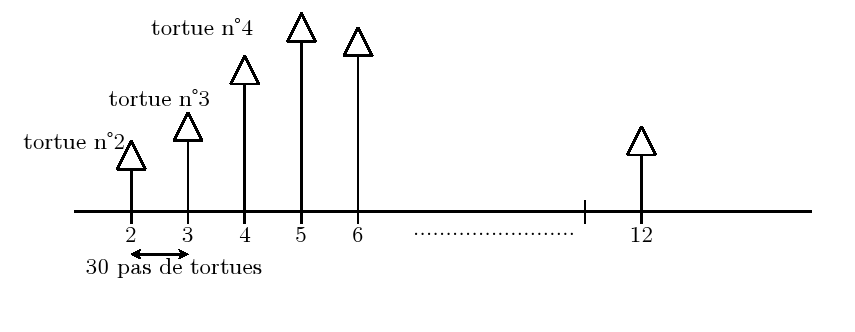
\includegraphics[scale=0.45]{images/somme-des-schema.png}
\end{center}
\vspace{0.5cm}
Sur le principe, chaque tortue numérotée de 2 à 12 avancera d'un pas de tortue, lorsque le tirage de la somme des deux dés sera identique à son numéro. Par exemple, si les dés ont pour somme 8, la tortue numéro 8 avancera d'un pas. Toutes les tortues sont espacées de 30 pas de tortues horizontalement.\\ \\
On placera les tortues à l'aide des coordonnées.
\begin{itemize}
 \item  La tortue n\degre2 sera placée en $(-150;0)$
 \item  La tortue n\degre3 sera placée en $(-120;0)$
 \item  La tortue n\degre4 sera placée en $(-90;0)$
 \item  La tortue n\degre5 sera placée en $(-60;0)$\\
\begin{minipage}{8 cm}
\begin{center}
 $\vdots$
\end{center}
\end{minipage}
\end{itemize}
\begin{verbatim}
 fixetortue 2 fpos [-150 0]
 fixetortue 3 fpos [-120 0]
 fixetortue 4 fpos [-90 0]
 fixetortue 5 fpos [-60 0]
 fixetortue 6 fpos [-30 0]
.....
\end{verbatim}
Plutôt que de taper 11 fois quasiment la même ligne de commande, on peut automatiser cela en utilisant la primitive \texttt{repetepour}. A l'aide de cette primitive, on peut affecter à une variable une succession de valeurs prises dans un intervalle à espaces réguliers. Ici, on veut que la variable \texttt{:i} prenne successivement les valeurs 2, 3, 4, ... , 12. On tapera:\\
\texttt{repetepour [i 2 12] [ liste des instructions à exécuter ]}\\ \\
Pour placer les tortues, on crée donc la procédure \texttt{initialise}
\begin{verbatim}
pour initialise
  ve ct
  repetepour [i 2 12] [ 
      # On place la tortue
      fixetortue :i fpos liste -150+(:i-2)*30 0
      # On écrit le numéro de la tortue juste en dessous 
      lc re 15 etiquette :i av 15 bc 
  ]
fin
\end{verbatim}

Bien comprendre la formule \texttt{-150+(:i-2)*30}. On part de -150, puis à chaque nouvelle tortue on rajoute 30. (Tester avec les différentes valeurs de \texttt{:i} si vous n'êtes pas convaincu)\\ \\
Au final on obtient le programme suivant:
\begin{verbatim}
pour lancer
 retourne 1+hasard 6
fin

pour initialise
  ve ct
  repetepour [i 2 12] [ 
      # On place la tortue
      fixetortue :i fpos liste -150+(:i-2)*30 0
      # On écrit le numéro de la tortue juste en dessous 
      lc re 15 etiquette :i av 15 bc 
  ]
fin

pour demarrer
initialise
# On effectue 1000 tentatives
repete 1000 [
  donne "somme lancer+lancer
  fixetortue :somme av 1
]
# On affiche les fréquences de tirage
repetepour [i 2 12] [
  fixetortue :i
  # L'ordonnée de la tortue représente le nombre de tirages
  soit "effectif dernier pos 
  lc av 10 tg 90 av 10 td 90 bc etiquette :effectif/1000*100
]
fin
\end{verbatim}
\pagebreak
Voici une généralisation de ce programme. Ici, on demandera à l'utilisateur le nombre de dés souhaités ainsi que le nombre de lancers à effectuer.
\begin{verbatim}
pour lancer
soit "somme 0
repete :des [
   soit "somme :somme+1 +hasard 6
 ]
retourne :somme
fin

pour initialise
  ve ct fixemaxtortues :max+1
  repetepour ph liste "i :min :max [ 
      # On place la tortue
      fixetortue :i fpos liste (:min-:max)/2*30+(:i-:min)*30 0
      # On écrit le numéro de la tortue juste en dessous 
      lc re 15 etiquette :i av 15 bc 
  ]
fin

pour demarrer
lis [Nombre de dés:] "des
si non nombre? :des [ec [Le nombre rentré n'est pas valide!] stop]
donne "min :des
donne "max 6*:des
lis [Nombre de lancers à effectuer] "tirages
si non nombre? :tirages [ec [Le nombre rentré n'est pas valide!] stop]
initialise
# On effectue 1000 tentatives
repete :tirages [
  fixetortue lancer av 1
]
# On affiche les fréquences de tirage
repetepour ph liste "i :min :max [
  fixetortue :i
  # L'ordonnée de la tortue représente le nombre de tirages
  soit "effectif dernier pos 
  # On arrondit à 0,1
  lc av 10 tg 90 av 10 td 90 bc etiquette (arrondi :effectif/:tirages*1000)/10
]
fin

\end{verbatim}
\chapter{Thème: Approximation probabilistique de $\pi$}
{ }\hfill\textbf{Niveau:} Avancé\\ \\
\noindent \textsc{Avertissement:} Quelques notions de mathématiques sont nécessaires pour bien appréhender ce chapitre.
\section{Notion de pgcd (plus grand commun diviseur)}
\noindent 
Etant donné deux nombres entiers, leur pgcd désigne leur plus grand commun diviseur. \\
\begin{itemize}
\item Par exemple, 42 et 28 ont pour pgcd 14 (c'est le plus grand nombre possible qui divise à la fois 28 et 42)
\item 25 et 55 ont pour pgcd 5.
\item 42 et 23 ont pour pgcd 1.
\end{itemize}
Lorsque deux nombres ont pour pgcd 1, on dit qu'ils sont premiers entre eux. Ainsi sur l'exemple précédent, 42 et 23 sont premiers entre eux. Cela signifie qu'ils n'ont aucun diviseur commun hormis 1 (bien sûr, il divise tout entier!).
\section{Algorithme d'Euclide}
\noindent Pour déterminer le pgcd de deux nombres, on peut utiliser une méthode appelée algorithme d'Euclide: (Ici, on ne démontrera pas la validité de cet algorithme)\\ \\
Voici le principe :
Étant donnés deux entiers positifs $a$ et $b$, on commence par tester si $b$ est nul. Si oui, alors le PGCD est égal à $a$. Sinon, on calcule $r$, le reste de la division de $a$ par $b$. On remplace $a$ par $b$, puis $b$ par $r$, et on recommence le procédé. \\
Calculons par exemple, le pgcd de 2160 et 888  par cet algorithme avec les étapes suivantes:
\begin{center}
$\begin{array}{ccc}
a & b & r\\
2160 & 888 & 384 \\
888 & 384 & 120 \\
384 & 120 & 24 \\
120 & 24 & 0 \\
24 & 0 & \\
\end{array}$
\end{center}
Le pgcd de 2160 et 888 est donc 24. Il n'y pas de plus grand entier qui divise ces deux nombres.
(En fait $2160=24\times90$ et $888=24\times37$)\\
Le pgcd est en fait le dernier reste non nul.
\section{Calculer un pgcd en \logo}
\noindent Un petit algorithme récursif permet de calculer le pgcd de deux nombres \texttt{:a} et \texttt{:b}
\begin{verbatim}
pour pgcd :a :b
si (reste :a :b)=0 [retourne :b][retourne pgcd :b reste :a :b] 
fin

ecris pgcd 2160 888 
24
\end{verbatim}
Remarque: On est obligé de mettre des parenthèses sur \texttt{reste :a :b}, sinon l'interpréteur va chercher à évaluer \texttt{:b = 0}. Pour éviter ce problème de parenthésage, écrire: \texttt{si 0=reste :a :b}

\section{Calculer une approximation de $\pi$}
\noindent En fait, un résultat connu de théorie des nombres établit que la probabilité que deux entiers pris au hasard soient premiers entre eux est de $\dfrac{6}{\pi^2}\approx 0,6079$. Pour essayer de retrouver ce résultat, voilà ce que l'on va faire:
\begin{itemize}
\item Prendre deux nombres au hasard entre 0 et 1 000 000.
\item Calculer leur pgcd
\item Si leur pgcd vaut 1. Rajouter 1 à une variable compteur.
\item Répéter l'expérience 1000 fois
\item La fréquence des couples de nombres premiers entre eux s'obtiendra en divisant la variable compteur par 1000 (le nombre d'essais).
\end{itemize}
\begin{verbatim}

pour test
# On initialise la variable compteur à 0
donne "compteur 0
repete 1000 [ 
  si (pgcd hasard 1000000 hasard 1000000)=1 [donne "compteur :compteur+1]
]
ecris [frequence:]
ecris :compteur/1000
fin

\end{verbatim}
Note: De même que précédemment, On est obligé de mettre des parenthèses sur \texttt{pgcd hasard 1000000 hasard 1000000}, sinon l'interpréteur va chercher à évaluer $1\ 000\ 000 = 1$. Pour éviter ce problème de parenthésage, écrire: \texttt{si 1=pgcd hasard 1000000 hasard 1000000}\\ \\
On lance le programme \texttt{test}.
\begin{verbatim}
test
0.609
test
0.626
test
0.597
\end{verbatim}
On obtient des valeurs proches de la valeur théorique de 0,6097. Ce qui est remarquable est que cette fréquence est une valeur approchée de $\dfrac{6}{\pi^2}$.\\
 Si je note $f$ la fréquence trouvée, on a donc: $f\approx \dfrac{6}{\pi^2}$ \\
Donc $\pi^2\approx\dfrac{6}{f}$ et donc $\pi\approx\sqrt{\dfrac{6}{f}}$.\\
Je m'empresse de rajouter cette approximation dans mon programme, je transforme la fin de la procédure \texttt{test}:
\begin{verbatim}

pour test
# On initialise la variable compteur à 0
donne "compteur 0
repete 1000 [ 
  si 1=pgcd hasard 1000000 hasard 1000000 [donne "compteur :compteur+1]
]
# On calcule la frequence
donne "f :compteur/1000
# On affiche la valeur approchée de pi
ecris phrase [approximation de pi:] racine (6/:f)
fin
test
approximation de pi: 3.164916190172819
test
approximation de pi: 3.1675613357997525
test
approximation de pi: 3.1008683647302115
\end{verbatim}
 Bon, je modifie mon programme de tel sorte que quand je le lance, je précise le nombre d'essais souhaités. J'ai dans l'idée d'essayer avec 10000 essais, voilà ce que j'obtiens sur mes trois premières tentatives:
\begin{verbatim}
pour test :essais
# On initialise la variable compteur à 0
donne "compteur 0
repete :essais [ 
  si 1=pgcd hasard 1000000 hasard 1000000 [donne "compteur :compteur+1]
]
# On calcule la frequence
donne "f :compteur/:essais
# On affiche la valeur approchée de pi
ecris phrase [approximation de pi:] racine (6/:f)
fin

test 10000
approximation de pi: 3.1300987144363774
test 10000
approximation de pi: 3.1517891481565017
test 10000
approximation de pi: 3.1416626832299914
\end{verbatim} 
 Pas mal, non?
\section{Compliquons encore un peu: $\pi$ qui génère $\pi$.....}
Qu'est-ce qu'un entier aléatoire? Est-ce qu'un entier pris au hasard antre 1 et 1 000 000 est réellement représentatif d'un entier aléatoire quelconque? On s'aperçoit très vite que notre modélisation ne fait qu'approcher le modèle idéal. Bien, c'est justement sur la façon de générer le nombre aléatoire que nous allons effectuer quelques changements... Nous n'allons plus utiliser la primitive \texttt{hasard} mais utiliser la séquence des décimales de $\pi$. Je m'explique: les décimales de $\pi$ ont toujours intrigué les mathématiciens par leur manque d'irrégularité, les chiffres de 0 à 9 semblent apparaître en quantité à peu près égales et de manière aléatoire. On ne peut prédire la prochaine décimales à l'aide des précédentes. Nous allons voir ci-après comment générer un nombre alatoire à l'aide des décimales de $\pi$. Tout d'abord, il va vous falloir récupérer les premières décimales de pi (par exemple un million).
 \begin{itemize}
 \item Il existe des petits programmes qui font cela très bien.  Je conseille PiFast pour Windows et ScnhellPi pour Linux.
 \item Récupérer ce fichier sur le site de \xlogo: 
\begin{center}
\texttt{http://downloads.tuxfamily.org/xlogo/common/millionpi.txt} 
\end{center}
 \end{itemize}
Pour créer nos nombres aléatoires, bous prendrons des paquets de 8 chiffres dans la suite des décimales de $\pi$. Explication, le fichier commence ainsi:\\
$\underbrace{3.1415926}_{\textrm{Premier nombre}}\underbrace{53589793}_{\textrm{Deuxième nombre}}\underbrace{23846264}_{\textrm{Troisième nombre}}338327950288419716939$ etc\\ \\

J'enlève le \og . \fg du 3.14 .... qui risque de nous ennuyer quand on extraiera les décimales. Bien, tout est en place, nous créons une nouvelle procédure appelée \texttt{hasardpi} et modifions légèrement la procédure \texttt{test}
\begin{verbatim}
pour pgcd :a :b
si (reste :a :b)=0 [retourne :b][retourne pgcd :b reste :a :b] 
fin

pour test :essais
# On ouvre un flux repéré par le chiffre 1 vers le fichier millionpi.txt
# (ici, supposé être dand le répertoire courant 
# sinon utiliser fixerepertoire et un chemin absolu)
ouvreflux 1 "millionpi.txt
# Affecte à la variable ligne la première ligne du fichier millionpi.txt
donne "ligne premier lisligneflux 1
# On initialise la variable compteur à 0
donne "compteur 0
repete :essais [
  si 1=pgcd hasardpi 7 hasardpi 7 [donne "compteur :compteur+1]
]
# On calcule la frequence
donne "f :compteur/:essais
# On affiche la valeur approchée de pi
ecris phrase [approximation de pi:] racine (6/:f)
fermeflux 1
fin
pour hasardpi :n
soit "nombre "
repete :n [
# S'il n'y plus de caractere sur la ligne
si 0=compte :ligne [donne "ligne premier lisligneflux 1]
# On donne à la variable caractere la valeur du premier caractere de la ligne
donne "caractere premier :ligne
# puis on enleve ce premier caractere de la ligne.
donne "ligne saufpremier :ligne
donne "nombre mot :nombre :caractere
]
retourne :nombre
fin

test 10
approximation de pi: 3.4641016151377544 
test 100
approximation de pi: 3.1108550841912757 
test 1000
approximation de pi: 3.081180112566604 
test 10000
approximation de pi: 3.1403714651066386 
test 70000
approximation de pi: 3.1361767950325627
\end{verbatim}
On retrouve donc une approximation du nombre $\pi$ à l'aide de ses propres décimales!\\ 
Il est encore possible d'améliorer ce programme en indiquant par exemple le temps mis pour le calcul. On rajoute alors en première ligne de la procedure test:\\
\texttt{donne "debut temps}\\
On rajoute juste avant \texttt{fermeflux 1}:\\
\texttt{ecris phrase [Temps mis: ] temps - :debut}\\
\chapter{Thème: Eponge de Menger}
{ }\hfill\textbf{Niveau:} Avancé\\ \\
Dans ce chapitre, nous allons construire un solide fractal appelé l'éponge de Menger. Voici les premières itérations pour contruire ce solide:
\begin{center}
\begin{minipage}{6cm}
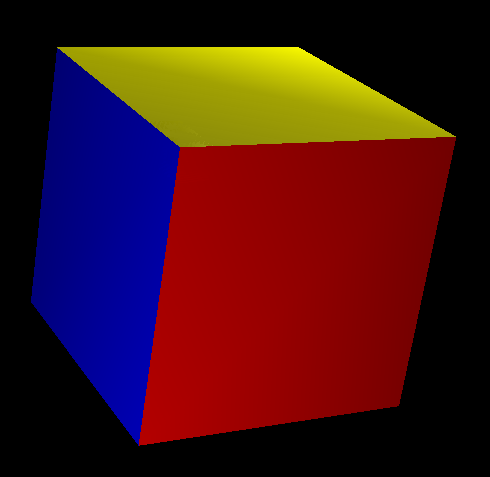
\includegraphics[width=6cm]{images/menger0.png}
\begin{center}
 \textbf{Etape 0}
\end{center}
\end{minipage}
\begin{minipage}{6cm}
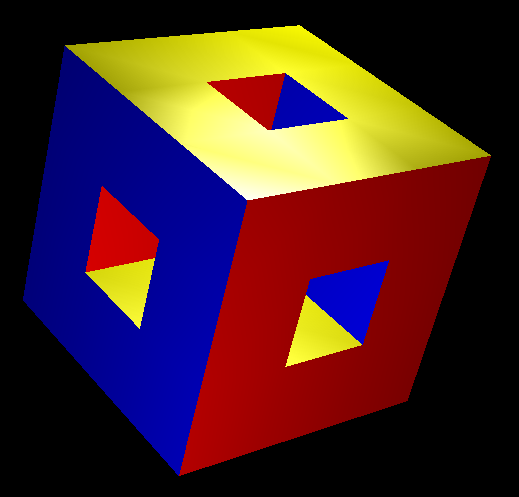
\includegraphics[width=6cm]{images/menger1.png}
\begin{center}
 \textbf{Etape 1}
\end{center}
\end{minipage}
\\
\begin{minipage}{6cm}
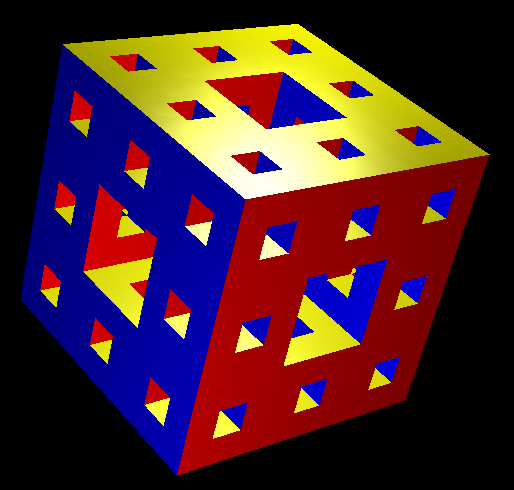
\includegraphics[width=6cm]{images/menger2.png}
\begin{center}
 \textbf{Etape 2}
\end{center}
\end{minipage}
\begin{minipage}{6cm}
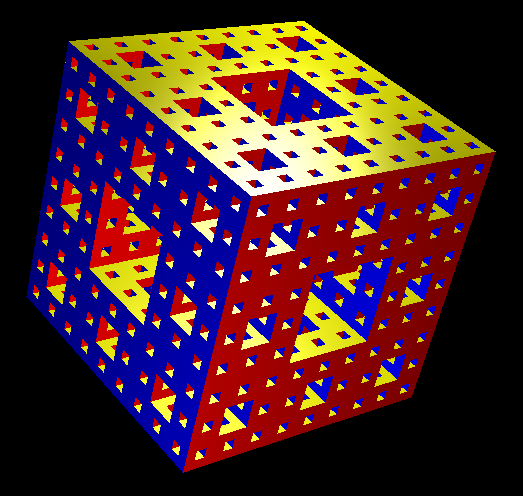
\includegraphics[width=6cm]{images/menger3.png}
\begin{center}
 \textbf{Etape 3}
\end{center}
\end{minipage}
\end{center}
Le chapitre se décompose en deux parties:
\begin{itemize}
 \item Tout d'abord, nous montrerons comment créer ce solide aisément en utilisant la récursivité.
 \item Dans un deuxième temps, on essaiera d'optimiser le tracé afin de tracer une éponge de Menger d'ordre~4.
\end{itemize}
\section{En utilisant la récursivité}
\noindent Considérons une éponge de menger d'ordre $n$ dont le côté mesure $L$.\\
\begin{center}
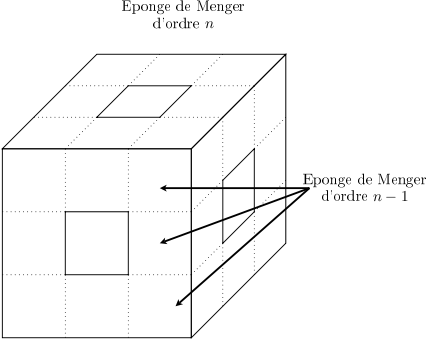
\includegraphics{images/menger-schema01.png}
\end{center}
Le schéma montre bien que cette éponge est constitué en fait de 20 éponges de Menger d'ordre $n-1$ ayant chacune un côté de $\dfrac{L}{3}$. La structure récursive de l'éponge est ainsi mise en évidence.\\ \\
\textbf{Le programme:}
\begin{verbatim}
# Commande principale: eponge 3
pour cube :l
si :compteur=10000 [vue3d]
# Couleur des faces latérales
soit "couleurs [jaune magenta cyan bleu]
# faces latérales
repete 4 [fcc exec item compteur :couleurs carre :l td 90 av  :l tg 90 rd 90]
# Dessous
fcc rouge pique 90 carre :l cabre 90
av :l pique 90 fcc vert carre :l cabre 90 re :l
fin

pour carre :c
donne "compteur :compteur+1
polydef
repete 4 [av :c td 90]
polyfin
fin

# Eponde de Menger 
# p: profondeur de récursivité
# l: Longueur du grand cube.
pour menger :l :p
si :p=0 [cube :l] [
  soit "p :p-1  
  soit "l :l/3
  #face avant
  repete 3 [menger :l :p av :l] re 3*:l
  td 90 av :l tg 90
  menger :l :p av 2*:l menger :l :p re 2*:l
  td 90 av :l tg 90
  repete 3 [menger :l :p av :l] re 3*:l
  #Côté droit 
 pique 90 av :l cabre 90 
  menger :l :p  av 2*:l menger :l :p re 2*:l
  pique 90 av :l cabre 90 
  repete 3 [menger :l :p av :l] re 3*:l
  tg 90 av :l td 90
  menger :l :p  av 2*:l menger :l :p re 2*:l
  tg 90 av :l td 90
  repete 3 [menger :l :p av :l] re 3*:l
  pique 90 re :l cabre 90
  menger :l :p  av 2*:l menger :l :p re 2*:l
   pique 90 re :l cabre 90
]
fin

pour eponge :p
ve ct donne "compteur 0 perspective fcfg 0 menger 800 :p 
tape [Nombre de polygone: ] ec :compteur 
vue3d
fin
\end{verbatim}
Ce programme comprend quatre procédures:
\begin{itemize}
 \item \texttt{carre :c}\\
Cette procédure trace un carré de côté \texttt{:c}. De plus, ce polygone est enregistré par le modeleur 3D. La variable \texttt{compteur} est chargée de dénombrer le nombre de polygones dessinés.
 \item \texttt{cube :l}\\
Cette procédure trace un cube de côté \texttt{:l}. Elle utilise bien sûr la procédure \texttt{carre}
 \item \texttt{menger :l :p}\\
Cette procédure est la clé du programme, elle dessine un motif de Menger d'ordre $p$ et dont le côté mesure $l$. Ce motif est créé de manière récursive de manière tout à fait naturelle en exploitant le schéma précédent.
 \item \texttt{eponge :p}\\
Cette procédure trace une eponge de Menger d'ordre $p$ et de côté 800 puis l'affiche dans le modeleur 3D.
\end{itemize}
\vfill
\pagebreak
\section{Deuxième approche: objectif solide d'ordre 4}
Le programme précédent a pour principal avantage d'exploiter la structure naturellement récursive du solide fractal. On peut noter que cette même méthode peut être réemployer pour générer d'autres solides fractals, ou plus simplement, d'autres courbes fractales. En tout cas, La conséquence immédiate de l'approche récursive est un code court et simple à comprendre. Malheureusement, on s'aperçoit qu'une éponge d'ordre 3 nécessite déjà 48 000 polygônes. Il faut alors régler la mémoire allouée à XLogo à 256 Mo dans le panneau des préférences pour que le programme puisse s'exécuter entièrement. \\ \\
Si l'on souhaite tracer une éponge de Menger d'ordre 4, on va vite être bloqué par un dépassement mémoire. Nous allons voir dans cette partie un programme basé sur un algorithme complètement différent, il permettra de créer une éponge de Menger d'ordre 0,1,2,3 ou 4.
\subsection{Le tapis de Sierpinski}
\noindent L'éponge de Menger est en fait la généralisation en 3 dimensions d'une figure du plan appelée le tapis de Sierpinski. Voici les premières itérations de cette figure:\\ \\
\begin{minipage}{4.5cm}
\begin{center}
 
\includegraphics[width=4.5cm]{images/carpet0.png}\\
\textbf{Etape 0}
\end{center}
\end{minipage}
\begin{minipage}{4.5cm}
\begin{center}
 
\includegraphics[width=4.5cm]{images/carpet1.png}\\
\textbf{Etape 1}
\end{center}
\end{minipage}
\begin{minipage}{4.5cm}
\begin{center}
 
\includegraphics[width=4.5cm]{images/carpet2.png}\\
\textbf{Etape 2}
\end{center}
\end{minipage}
\begin{minipage}{4.5cm}
\begin{center}
 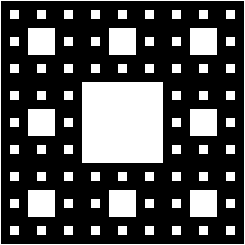
\includegraphics[width=4.5cm]{images/carpet3.png}\\
\textbf{Etape 3}
\end{center}
\end{minipage}\\ 
\vspace*{0.5cm}\\
Le motif présent sur chacune des faces d'une éponge de Menger d'ordre $p$ est un tapis de Sierpinski d'ordre $p$.
\subsection{Tracer un tapis de Sierpinski d'ordre $p$}
L'objectif est déjà de réussir à minimiser le nombre de polygônes nécessaires pour dessiner un tapis de Sierpinski. L'exemple suivant explique le procédé employé pour créer un tapis de Sierpinski d'ordre 3. Ici, le carré initial comporte donc $3^3=27$ lignes et 27 colonnes. On écrit en base 3 le numéro de chacune des lignes et de chacune des colonnes.
\begin{itemize}
 \item [\textbullet]\textbf{Première étape:} Pour toutes les lignes dont le numéro ne comporte aucun 1, on trace une ligne de 27 carreaux. Par symétrie, on effectue la même opération sur les colonnes.\\
\begin{center}
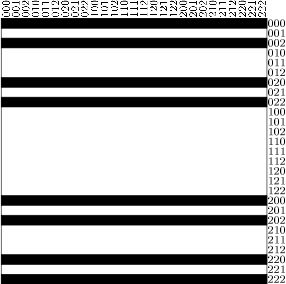
\includegraphics{images/menger-schema02.png}
\includegraphics{images/menger-schema03.png}
\end{center}
\vspace{0.2cm}
\item [\textbullet] \textbf{Deuxième étape:} On s'intéresse à présent aux lignes dont le numéro comporte un seul 1 en première position. On trace successivement par alternance des rectangles de longueur 9 carreaux. On reporte alors cette opération sur les colonnes par symétrie .\\
\begin{center}
\includegraphics{images/menger-schema04.png}
\end{center} 
\item [\textbullet] \textbf{Troisième étape:} On s'intéresse à présent aux lignes dont le numéro comporte un seul 1 en deuxième position. On trace successivement par alternance des rectangles en suivant le schéma $[3\ 3\ 6\ 3\ 6\ 3\ 3]$. (3 carreaux tracés, 3 non tracés, 6 tracés etc...) On reporte alors par symétrie cette opération sur les colonnes.
\begin{center}
\includegraphics{images/menger-schema05.png}
\end{center}
\item [\textbullet] \textbf{Dernière étape:} On s'intéresse alors aux lignes dont le numéro comporte deux 1 placés aux premières positions. On trace successivement par alternance des rectangles en suivant le schéma $[3\ 3\ 3\ 9\ 3\ 3\ 3]$. On reporte ensuite cette opération sur les colonnes.
\begin{center}
\includegraphics{images/menger-schema06.png}
\end{center}
\end{itemize}
La construction du tapis de Sierpinski d'ordre 3 est alors terminée. Pour créer ce tapis, il a fallu utiliser en tout: $16+16+32+16=80$ polygones.
\subsection{Différents schémas de colonnes possibles}
Pour récapituler la construction précédente, voici les différents types de schémas de colonnes suivant leur numéro de lignes. (Le symbole * désigne le chiffre 0 ou le chiffre 2)
\begin{center}
 \begin{tabular}{|c|c|}
 \hline
Numéro de ligne du type & Schéma à appliquer \\
\hline
*** & 27 \\ 
\hline
1** &  9 9 9 \\
\hline
*1* & 3 3 6 3 6 3 3\\
\hline
11* & 3 3 3 9 3 3 3\\
\hline
\end{tabular}
\end{center}

Sur le même principe, pour créer un tapis d'ordre 4, on utilisera un carré avec $3^4=81$ carreaux. Les numéros de ligne et de colonne possèderont donc 4 chiffres dans leur décomposition en base 3. Pour chaque type de numéro de lignes, voici le schéma à appliquer (le symbole * désigne le chiffre 0 ou le chiffre 2):
\begin{center}
 \begin{tabular}{|c|c|}
 \hline
Numéro de ligne du type & Schéma à appliquer \\
\hline
 **** & 81 \\ 
\hline
1*** &  27 27 27 \\
\hline
*1** & 9 9 18 9 18 9 9 \\
\hline
**1* & 3 3 6 3 6 3 6 3 6 3 6 3 6 3 6 3 6 3 3 \\
\hline
*11* &  3 3 3 9 3 3 6 3 3 9 3 3 6 3 3 9 3 3 3 \\
\hline
1*1* & 3 3 6 3 6 3 3 27 3 3 6 3 6 3 3 \\
\hline
11** & 9 9 9 27 9 9 9 \\
\hline
111*& 3 3 3 9 3 3 3 27 3 3 3 9 3 3 3 \\
\hline
\end{tabular}\\
496 polygônes sont alors nécessaires pour tracer un tapis de Sierpinski d'ordre 4.\\
\end{center}
Enfin, voici les chémas de constructions de colonnes pour les solides d'ordre 2:
\begin{center}
  \begin{tabular}{|c|c|}
 \hline
Numéro de ligne du type & Schéma à appliquer \\
\hline
** &  9 \\
\hline
1* & 3 3 3 \\ 
\hline
\end{tabular}
\end{center}
\subsection{Le programme}
\begin{verbatim}
 #trace un tapis de Sierpinski d'ordre :p et de taille :size
pour carpet :size :p
donne "unit :size/(puissance 3 :p)
si :p=0 [ rec :size :size stop]
si :p=1 [repete 4 [rec :size :unit av :size td 90 ] stop]
repetepour (liste "x 1 puissance 3 :p) [
  soit "cantorx cantor :x :p []
# On ne trace pas les éléments ayant un 1 en derniere position
si  non (1=dernier :cantorx)  [
  soit "nom evalue saufdernier :cantorx "
  drawColumn :x rprop "map :nom
  ]
]  
fin

# Retourne la décomposition en base 3 du nombre x
# p indice de profondeur 3^p
# :list liste vide au démarrage

pour cantor :x :p :list
si :p=0 [retourne :list] 
soit "a puissance 3 :p-1
si :x<= :a [
  retourne cantor  :x :p-1  phrase :list 0] 
  [ si :x<=2*:a [retourne cantor  :x-:a :p-1  phrase :list 1] 
  retourne cantor :x-2*:a :p-1 phrase :list 0]
fin

# Trace la colonne numéro x en respectant le schéma de construction défini dans la liste
pour drawcolumn :x :list
  lc  td 90 av (:x-1)*:unit tg 90  bc des :list
  lc tg 90 av (:x-1)*:unit td 90 av :x*:unit td 90 bc des :list
lc tg 90 re :x*:unit bc
fin

# Trace un rectangle de dimensions données
# Le polygone est enregistrées par le viewer3d
pour rec :lo :la
donne "compteur :compteur+1
polydef
repete 2 [av :lo td 90 av :la td 90]
polyfin
fin

# Initialise les différentes colonnes possibles pour les tapis d'ordre 1 à 4
pour initmap
dprop "map 111 [3 3 3 9 3 3 3 27 3 3 3 9 3 3 3]
dprop "map 110 [9 9 9 27 9 9 9]
dprop "map 101 [3 3 6 3 6 3 3 27 3 3 6 3 6 3 3]
dprop "map 011 [3 3 3 9 3 3 6 3 3 9 3 3 6 3 3 9 3 3 3]
dprop "map 000 [81]
dprop "map 100 [27 27 27]
dprop "map 010 [9 9 18 9 18 9 9]
dprop "map 001 [3 3 6 3 6 3 6 3 6 3 6 3 6 3 6 3 6 3 3]
dprop "map 01 [3 3 6 3 6 3 3]
dprop "map 00 [27]
dprop "map 10 [9 9 9]
dprop "map 11 [3 3 3 9 3 3 3]
dprop "map 1 [3 3 3]
dprop "map 0 [9]
fin

# Si la decomposition est [1 0 1] --> retourne 101
pour evalue :list :mot
  si vide? :list [retourne :mot]
  [
  soit "mot mot :mot premier :list
  retourne evalue saufpremier :list :mot  
]
fin
# Trace les blocs de rectangles de chaque colonne par alternance
pour des :list
soit "somme 0
repetepour (liste "i 1 compte :list) [
   soit "element item :i :list
    soit "somme :element+:somme 
  si pair? :i [lc av :element*:unit bc ] [rec :element*:unit :unit av :element*:unit]  
]
lc re  :somme * :unit bc
fin

# Teste si un nombre est pair
pour pair? :i
retourne 0=reste :i 2
fin

pour tapis :p
ve perspective ct initMap
donne "compteur 0
carpet 810 :p
tape "Nombre\ de\ polygones:\  ec :compteur 
vue3d
fin
\end{verbatim}
\texttt{tapis 3} dessine un tapis de Sierpinski d'ordre 3 de côté 810. Voilà, nous sommes prêts à passer à l'éponge de Menger!

\subsection{L'éponge de Menger d'ordre 4}
L'éponge de Menger possède de multiples propriétés de symétrie. Pour la générer nous allons tracer les différentes sections suivant le plan $(xOy)$ puis reporter ces figures suivant $(yOz)$ et $(xOz)$. Pour bien expliquer ce qui se passe, restons sur l'exemple de l'éponge d'ordre 3:\\
Lorsque l'on coupe l'éponge par un plan vertical, on peut obtenir quatre motifs différents:\\
\vspace*{0.6cm}
 \begin{center}
\includegraphics{images/menger-schema07.png}\\ \vspace{0.5cm}
\includegraphics{images/menger-schema08.png}\\ \vspace{0.5cm}
\includegraphics{images/menger-schema09.png}\\ \vspace{0.5cm}
\includegraphics{images/menger-schema10.png}\\ 
\end{center}
Pour tracer une éponge d'ordre 3, nous allons parcourir les nombres de 1 à 27, c'est à dire de 001 à 222 en base 3. Pour chaque numéro, on appliquera la section adéquate que l'on reportera suivant les 3 directions $(Ox)$, $(Oy)$ et $(Oz)$.
\subsubsection{Le code}
\noindent Le programme suivant permet de tracer les solides de Menger d'ordre 0,1,2,3,4. Le nombre de procédures est important donc j'apporterai quelques éclaircissements ensuite.
\begin{verbatim}
#trace un tapis de Sierpinski d'ordre :p et de taille :size
pour carpet :size :p
donne "unit :size/(puissance 3 :p)
si :p=0 [ rec :size :size stop]
si :p=1 [repete 4 [rec :size :unit av :size td 90 ] stop]
repetepour (liste "x 1 puissance 3 :p) [
  soit "cantorx cantor :x :p []
# On ne trace pas les éléments ayant un 1 en derniere position
si  non (1=dernier :cantorx)  [
  soit "nom evalue saufdernier :cantorx "
  drawColumn :x rprop "map :nom
  ]
]  
fin

# Retourne la décomposition en base 3 du nombre x
# p indice de profondeur 3^p
# :list liste vide au démarrage

pour cantor :x :p :list
si :p=0 [retourne :list] 
soit "a puissance 3 :p-1
si :x<= :a [
  retourne cantor  :x :p-1  phrase :list 0] 
  [ si :x<=2*:a [retourne cantor  :x-:a :p-1  phrase :list 1] 
  retourne cantor :x-2*:a :p-1 phrase :list 2]
fin

# Trace la colonne number x en respectant le schéma de construction défini dans la liste
pour drawcolumn :x :list
  lc  td 90 av (:x-1)*:unit tg 90  bc des :list
  lc tg 90 av (:x-1)*:unit td 90 av :x*:unit td 90 bc des :list
lc tg 90 re :x*:unit bc
fin

# Trace un rectangle de dimensions données
# Le polygone est enregistrées par le viewer3d
pour rec :lo :la
donne "compteur :compteur+1
polydef
repete 2 [av :lo td 90 av :la td 90]
polyfin
fin

# Initialise les différentes colonnes possibles pour les tapis d'ordre 1 à 4
pour initmap
dprop "map 111 [3 3 3 9 3 3 3 27 3 3 3 9 3 3 3]
dprop "map 110 [9 9 9 27 9 9 9]
dprop "map 101 [3 3 6 3 6 3 3 27 3 3 6 3 6 3 3]
dprop "map 011 [3 3 3 9 3 3 6 3 3 9 3 3 6 3 3 9 3 3 3]
dprop "map 000 [81]
dprop "map 100 [27 27 27]
dprop "map 010 [9 9 18 9 18 9 9]
dprop "map 001 [3 3 6 3 6 3 6 3 6 3 6 3 6 3 6 3 6 3 3]
dprop "map 01 [3 3 6 3 6 3 3]
dprop "map 00 [27]
dprop "map 10 [9 9 9]
dprop "map 11 [3 3 3 9 3 3 3]
dprop "map 1 [3 3 3]
dprop "map 0 [9]
fin

# Si la decomposition est [1 0 1] --> retourne 101
# Si la decomposition est [1 0 2] --> retourne 100
#  Les éléments de la liste sont concaténés en un mot. 
# De plus, es 2 sont remplacés par des zéros
pour evalue :list :mot
  si vide? :list [retourne :mot]
  [
  soit "first premier :list
  si :first=2 [soit "first 0] 
 soit "mot mot :mot :first
  retourne evalue saufpremier :list :mot  
]
fin
# Trace les blocs de rectangles de chaque colonne par alternance
pour des :list
soit "somme 0
repetepour (liste "i 1 compte :list) [
   soit "element item :i :list
    soit "somme :element+:somme 
  si pair? :i [lc av :element*:unit bc ] [rec :element*:unit :unit av :element*:unit]  
]
lc re  :somme * :unit bc
fin

# Teste si un nombre est pair
pour pair? :i
retourne 0=reste :i 2
fin

pour tapis :p
ve perspective ct initMap
donne "compteur 0
carpet 810 :p
tape "Nombre\ de\ polygones:\  ec :compteur 
vue3d
fin

# Supprime le dernier 1 dans la liste :list
pour deletelastone :list
repetepour (liste "i compte :list 1 moins 1) [
  soit "element item :i :list 
  si :element=1 [soit "list remplace :list :i 0 stop] [si :element=2 [stop]]
]
retourne :list
fin

# Eponge de Menger de taille donnée et de profondeur :p

pour menger :size :p
donne "unite :size/(puissance 3 :p)
repetepour (liste "z 1 puissance 3 :p) [
  soit "cantorz cantor :z :p []
  soit "last dernier :cantorz
  soit "cantorz saufdernier :cantorz
  si :last=0 [soit "order evalue deleteLastOne :cantorz "]  [soit "order evalue :cantorz "]
  soit "order mot "coupe :order
  draw3carpet :size :order :z
  lc cabre 90 av :unit pique 90 bc 
]
draw3carpet :size :order (puissance 3 :p)+1
fin

# Trace les tapis de Sierpinski d'ordre :p
# suivant chaque axe (Ox), (Oy) et (Oz)
# à l'altitude :z
pour draw3carpet :size :order :z
lc origine  
cabre 90 av (:z-1)*:unite pique 90 bc
fcc bleu exec :order :size
lc origine  
rg 90 av (:z-1)*:unite pique 90  bc
fcc jaune exec :order :size
lc origine  
cabre 90 av :size td 90 av (:z-1)*:unite pique 90 bc
fcc magenta exec :order :size 
fin


# Procédure principale
# Trace une eponge de Menger de profondeur p
pour eponge :p
ve perspective ct
soit "temps temps
initMap
donne "compteur 0
si :p=0 [cube 405] [menger 405 :p]
# Affiche le temps mis et le nombre de polygone nécessaire à la construction
tape "Nombre\ de\ polygones:\  ec :compteur 
tape "Temps\ mis:\  ec temps -:temps 
vue3d
fin

# Section pour le Menger d'ordre 2
pour coupe1 :size
repete 4 [carpet :size/3 1 lc av :size td 90 bc]
fin

pour coupe0 :size
carpet :size 2
fin

# Section pour le Menger d'ordre 3

pour coupe10 :size
repete 4 [carpet :size/3 2 lc av :size td 90 bc]
fin

pour coupe01 :size
repete 4 [repete 2 [coupe1 :size/3 lc av :size/3 bc] av :size/3 td 90]
fin

pour coupe11 :size
repete 4 [coupe1 :size/3 lc av :size td 90 bc]
fin


pour coupe00 :size
carpet :size 3
fin

# Section pour le Menger d'ordre 4
pour coupe000 :size
carpet :size 4
fin

pour coupe100 :size
repete 4 [carpet :size/3 3 lc av :size td 90 bc]
fin

pour coupe010 :size
repete 4 [repete 2 [coupe10 :size/3 lc av :size/3 bc] av :size/3 td 90]
fin

pour coupe001 :size
repete 4 [repete 2 [coupe01 :size/3 lc av :size/3 bc] av :size/3 td 90]
fin

pour coupe110 :size
repete 4 [coupe10 :size/3 lc av :size bc td 90 ]
fin

pour coupe111 :size
repete 4 [coupe11 :size/3 lc av :size td 90 bc]
fin

pour coupe101 :size
repete 4 [coupe01 :size/3 lc av :size td 90 bc]
fin

pour coupe011 :size
repete 4 [repete 2 [coupe11 :size/3 lc av :size/3 bc] av :size/3 td 90]
fin

pour coupe :size
carpet :size 1
fin

pour cube :size
repete 2 [
fcc bleu rec :size :size lc av :size pique 90 bc 
fcc jaune rec :size :size lc av :size pique 90  bc
]
fcc magenta
lc rg 90 tg 90 av :size td 90 bc rec :size :size
lc td 90 av :size tg 90 rd 90 td 90 av :size tg 90 rd 90 bc rec :size  :size
rg 90 tg 90 av :size td 90
fin

pour cubes
ve perspective ct
soit "temps temps
initMap
donne "compteur 0
repete 4 [si compteur=1 [cube 405] [menger 405 compteur-1] lc av 1000 td 90 bc ]
# Affiche le temps mis et le nombre de polygone nécessaire à la construction
tape "Nombre\ de\ polygones:\  ec :compteur 
tape "Temps\ mis:\  ec temps -:temps 
vue3d
fin
\end{verbatim}
Ensuite, on règle la mémoire allouée à \xlogo\ à 640 Mo: \texttt{eponge 4}
\begin{center}
 \includegraphics{images/menger-menger4.png}
\end{center}
\chapter{Thème: Système de Lindenmayer}
{ }\hfill\textbf{Niveau:} Avancé\\ \\
\noindent
Dans cette partie, certaines références sont issues:
\begin{itemize}
 \item  de la page Wikipedia sur les L-system: \texttt{http://fr.wikipedia.org/wiki/L-System}.
 \item du livre \og The Algorithmic Beauty of Plants \fg écrit par Przemyslaw Prusinkiewicz et Aristid Lindenmayer.
\end{itemize}
\vspace*{0.5cm}
Cette partie va traiter de la notion de  système de Lindenmayer ou L-system inventé en 1968 par le biologiste hongrois Aristid Lindenmayer. Un L-System est un ensemble de règles et de symboles qui modélisent un processus de croissance d'êtres vivants comme des plantes ou des cellules. Le concept central des L-Systems est la notion de réécriture. La réécriture est une technique pour construire des objets complexes en remplaçant des parties d'un objet initial simple en utilisant des règles de réécriture.\\ \\
Pour ce faire, les cellules sont modélisées à l'aide de symboles. À chaque génération, les cellules se divisent, i.e. un symbole est remplacé par un ou plusieurs autres symboles formant un mot.
\section{Définition formelle}
\noindent
Un L-System est une grammaire formelle qui comprend :
\begin{enumerate}
 \item Un alphabet $V$ : l'ensemble des variables du L-System. $V *$ est l'ensemble des "mots" que l'on peut construire avec les symboles de $V$, et $V +$ l'ensemble des mots contenant au moins un symbole.
 \item Un ensemble de valeur constantes $S$. Certains de ces symboles sont communs à tous les L-System. (Notamment quand on utilisera la tortue).
  \item Un axiome de départ $\omega$ choisi parmi $V +$ , c'est à dire l'état initial.
 \item Un ensemble de règles, noté $P$, de reproduction des symboles de $V$.
\end{enumerate}
Un L-System est alors noté $\{V,S,\omega,P\}$.\\ \\
Considérons le L-system suivant:
\begin{itemize}
 \item Alphabet : $V = \{A, B\}$
 \item Constantes : $S = \{\emptyset\}$
 \item Axiome de départ : $\omega = A$
 \item Régles : $\begin{array}{|l|}
\hline
A \rightarrow AB \\
B \rightarrow A \\ 
\hline
\end{array}
$
\end{itemize}
Les deux règles qui sont données sont les règles de réécriture du système. A chaque étape, $A$ est remplacé par la séquence $AB$, et $B$ est remplacé par $A$. Voici les premières itérations de ce système de Lindemayer:
\begin{center}
\includegraphics[width=8cm]{images/linden-arbre.png}
\end{center}
\begin{itemize}
\item Itération 1: $A$
\item Itération 2: $AB$
\item Itération 3: $ABA$
\item Itération 4: $ABAAB$
\end{itemize}
\vspace*{0.2cm}
Bien, bien... et concrètement?? Lisons la suite!
\section{Interprétation par la tortue}
\noindent Ce premier exemple vous a permis d'appréhender la notion de système de Lindenmayer sans toutefois peut-être discerner comment nous allons utiliser cela concrètement avec la tortue.\\ \\
C'est là que cela devient intéressant: Chacun des mots ainsi construits ne possède pas de signification particulière. On va alors attacher à chacune des lettres de la séquence, une commande à exécuter par la tortue et générer ainsi des dessins en 2D ou en 3D.
\subsection{Symboles usuels}
\begin{itemize}
 \item [\textbullet] $F$ : Se déplacer d’un pas unitaire ($\in V$)
 \item [\textbullet] $+$ : Tourner à gauche d’angle $\alpha$ $(\in S)$.
 \item [\textbullet] $-$ : Tourner à droite d’un angle $\alpha$ $(\in S)$.
 \item [\textbullet] $\&$ : Pivoter vers le bas d’un angle $\alpha$ $(\in S)$.
 \item [\textbullet] \textasciicircum : Pivoter vers le haut d’un angle $\alpha$ $(\in S)$.
 \item [\textbullet] \textbackslash: Roulez vers la gauche d’un angle $\alpha$ $(\in S)$.
 \item [\textbullet] $/$: Roulez vers la droite d’un angle $\alpha$ $(\in S)$.
 \item [\textbullet] $|$: Effectuer un demi-tour. Avec XLogo: \texttt{td 180}
\end{itemize}
\vspace*{0.2cm}
Prenons par exemple $\alpha=90$ et un déplacement unitaire de 10 pas de tortue, on obtient alors:
\begin{center}
 \begin{tabular}{|c|c|c|c|c|c|c|c|c|}
 \hline
Symbole & $F$ & $+$ & $-$ & $\&$ & \textasciicircum & \textbackslash& $/$ & $|$ \\
 \hline
Commande XLogo & \texttt{av 10}&\texttt{tg 90}&\texttt{td 90}&\texttt{pique 90}&\texttt{cabre 90}&\texttt{rg 90}&\texttt{rd 90}&\texttt{td 180}\\
 \hline
\end{tabular}
\end{center}
\subsection{Flocon de Koch}
Considérons le L-system:
\begin{itemize}
 \item [\textbullet] Etat initial: $F--F--F--$
 \item [\textbullet] Règle de production: $F \rightarrow F+F--F+F$
 \item [\textbullet] Angle $\alpha=60$\degre, le pas unitaire est divisé par 3 entre chaque itération.
\end{itemize}
Premières itérations:
\begin{center}
\begin{minipage}{7.5cm}
 \includegraphics[width=7.5cm]{images/linden-flocon1.png}
\end{minipage}
\begin{minipage}{7.5cm}
 \includegraphics[width=7.5cm]{images/linden-flocon2.png}
\end{minipage}\\
\begin{minipage}{7.5cm}
 \includegraphics[width=7.5cm]{images/linden-flocon3.png}
\end{minipage}
\begin{minipage}{7.5cm}
 \includegraphics[width=7.5cm]{images/linden-flocon4.png}
\end{minipage}
\end{center}
\noindent Programme en Logo:
\begin{verbatim}
 
pour flocon :p
donne "unit 300/puissance 3 :p-1
repete 3 [F :p-1 td 120]  
fin

pour f :p
si :p=0 [av :unit stop]
F :p-1 tg 60 F :p-1 td 120 F :p-1 tg 60
F :p-1 
fin

\end{verbatim}
\subsection{Courbe de Koch d'ordre 2}
\noindent Intéressons-nous le L-system suivant:
\begin{itemize}
 \item[\textbullet] Etat initial: $F-F-F-F$
 \item[\textbullet] Règle de production: $F\rightarrow F-F+F+FF-F-F+F$
\end{itemize}
Voici les premières représentations en utilisant $\alpha=90$ et en ajustant le pas unitaire de telle sorte que la figure fasse toujours la même taille:
\begin{center}
\begin{minipage}{7.5cm}
 \includegraphics[width=7.5cm]{images/linden-koch1.png}
\end{minipage}
\begin{minipage}{7.5cm}
 \includegraphics[width=7.5cm]{images/linden-koch2.png}
\end{minipage}\\
\begin{minipage}{7.5cm}
 \includegraphics[width=7.5cm]{images/linden-koch3.png}
\end{minipage}
\begin{minipage}{7.5cm}
 \includegraphics[width=7.5cm]{images/linden-koch4.png}
\end{minipage}
\end{center}
Il est alors très facile de créer le programme Logo permettant de générer ces dessins:
\begin{verbatim}
# p désigne l'itération
pour koch :p
# Entre chaque itération, la distance unitaire est divisée par 4
# Ici, la figure finale aura une taille de 600x600 au maximum
donne "unit 300/puissance 4 :p-1

repete 3 [F :p-1 tg 90] F :p-1 
fin

# La chaine de réécriture
pour F :p
si :p=0 [av :unit stop]
F :p-1 tg 90 F :p-1 td 90 F :p-1 td 90
F :p-1 F :p-1 tg 90 F :p-1 tg 90 F :p-1 td 90 F :p-1
fin
\end{verbatim}
\subsection{Courbe du dragon}
\begin{itemize}
 \item[\textbullet] Etat initial: $F$\\
 \item[\textbullet] Règle de production: $\begin{array}{|l|}
\hline
A\rightarrow A+B+ \\
B\rightarrow -A-B \\
\hline
\end{array}$ 
\end{itemize}
\begin{verbatim}
pour a :p
si :p=0 [av :unit stop]
a :p-1 tg 90 b :p-1 tg 90
fin

pour b :p
si :p=0 [av :unit stop]
td 90 a :p-1 td 90 b :p-1

fin

pour dragon :p
donne "unit 300/8/ :p  
a :p
fin
\end{verbatim}
\begin{center}
 \begin{minipage}{7cm}
 \includegraphics[width=7cm]{images/linden-dragon10.png}
 \begin{center}
  \texttt{dragon 10}
 \end{center}
\end{minipage}
 \begin{minipage}{7cm}
 \includegraphics[width=7cm]{images/linden-dragon15.png}
 \begin{center}
  \texttt{dragon 15}
 \end{center}
\end{minipage}
\end{center}

\subsection{Courbe de Hilbert en 3D}
\noindent L'exemple suivant traite de la courbe de Hilbert dans l'espace, c'est une courbe qui a la propriété de remplir parfaitement un cube quand on augmente le nombre d'itérations.\\ \\
Voici le L-system associé:
\begin{itemize}
 \item Etat initial: $A$
 \item Angle $\alpha=90$\degre, on divise la longueur unitaire par deux à chaque itération.\\
 \item Règle de production: $\begin{array}{|l|}
\hline
A\rightarrow B-F+CFC+F-D\&F \textrm{\textrm{\textasciicircum}} D-F+\&\&CFC+F+B// \\
B\rightarrow A\&F\textrm{\textrm{\textasciicircum}} CFB\textrm{\textasciicircum} F \textrm{\textasciicircum} D\textrm{\textasciicircum} \textrm{\textasciicircum}-F-D\textrm{\textasciicircum}|F\textrm{\textasciicircum} B|FC\textrm{\textasciicircum} F\textrm{\textasciicircum} A// \\
C\rightarrow|D\textrm{\textasciicircum}|F\textrm{\textasciicircum} B-F+C\textrm{\textasciicircum} F\textrm{\textasciicircum} A\&\&FA\&F\textrm{\textasciicircum} C+F+B\textrm{\textasciicircum} F\textrm{\textasciicircum} D// \\
D\rightarrow|CFB-F+B|FA\&F\textrm{\textasciicircum} A\&\&FB-F+B|FC// \\
\hline
\end{array}$
\end{itemize}
\begin{verbatim}
pour hilbert :p
ve perspective
donne "unit 400/puissance 2 :p
lignedef ftc :unit/2
a :p
lignefin
vue3d
fin

pour a :p
si :p=0 [stop]
b :p-1 td 90 av :unit tg 90  c :p-1 av :unit c :p-1
tg 90 av :unit td 90 d :p-1 pique 90 av :unit cabre 90 d :p-1
td 90 av :unit tg 90 pique 180 c :p-1 av :unit c :p-1
tg 90 av :unit tg 90 b :p-1 rd 180
fin

pour b :p
si :p=0 [stop]
a :p-1 pique 90 av :unit cabre 90 c :p-1 av :unit b :p-1 cabre 90 
av :unit cabre 90 d :p-1 cabre 180 td 90 av :unit td 90 d :p-1 cabre 90 
td 180 av :unit cabre 90 b :p-1 td 180 av :unit c :p-1 cabre 90 av :unit 
cabre 90 a :p-1 rd 180 
fin

pour c :p
si :p=0 [stop]
td 180 d :p-1 cabre 90 td 180 av :unit cabre 90 b :p-1 td 90 av :unit tg 90 
c :p-1 cabre 90 av :unit cabre 90 a :p-1 pique 180 av :unit a :p-1 pique 90 
av :unit cabre 90 c :p-1 tg 90 av :unit tg 90 b :p-1 cabre 90 av :unit cabre 90 
d :p-1 rd 180 
fin

pour d :p
si :p=0 [stop]
td 180 c :p-1 av :unit b :p-1 td 90 av :unit tg 90 b :p-1 td 180
av :unit a :p-1 pique 90 av :unit cabre 90 a :p-1 pique 180 av :unit
b :p-1 td 90 av :unit tg 90 b :p-1 td 180 av :unit c :p-1 rd 180
fin
\end{verbatim}
Et les premières itérations obtenues:
\begin{center}
\begin{minipage}{7cm}
 \includegraphics[width=7cm]{images/linden-hilbert1.png}
\end{minipage}
\begin{minipage}{7cm}
 \includegraphics[width=7.5cm]{images/linden-hilbert2.png}
\end{minipage}\\
\begin{minipage}{7cm}
 \includegraphics[width=7cm]{images/linden-hilbert3.png}
\end{minipage}
\begin{minipage}{7cm}
 \includegraphics[width=9cm]{images/linden-hilbert4.png}
\end{minipage}
\end{center}
\appendix
\chapter{Liste des primitives}
\label{liste-prim} Comme il a été indiqué auparavant, le contrôle de la tortue s'effectue
à l'aide de commandes internes appelées \og primitives \fg. Voici
une classification de ces primitives:


\section{Déplacement de la tortue, gestion du crayon et des couleurs}
\subsection{Déplacement}
\noindent Ce premier lot de primitives permet de déplacer la tortue.\\
\prim{avance, av}{n}
Fait avancer de n pas la tortue suivant l'orientation courante.\\
\prim{recule, re}{n}
Fait reculer de n pas la tortue suivant l'orientation courante.\\
\prim{tournedroite, td}{n}
Fait tourner la tortue de n degrés vers la droite par rapport à son
orientation actuelle.\\
\prim{tournegauche, tg}{n}
Fait tourner la tortue de n degrés vers la gauche par rapport à son
orientation actuelle.\\
\prim{cercle}{R}
Trace un cercle de rayon R autour de la tortue.\\
\prim{arc}{R cap1 cap2}
 Trace un arc de cercle de rayon R autour de la tortue. Cette arc est compris entre les caps cap1 et cap2.\\
\prim{origine}{}
 Replace la tortue à sa position initiale, c'est à dire au point de
coordonnées {[}0 0{]} et avec pour cap 0\\
\prim{fixeposition, fpos}{liste}
 Déplace la tortue au point de coordonnées spécifié à l'aide de la
liste des deux nombres.(abscisse puis ordonnée)\\
\prim{fixex}{x}
 Déplace la tortue horizontalement jusqu'au point d'abscisse x\\
\prim{fixey}{y}
 Déplace la tortue verticalement jusqu'au point d'ordonnée y\\
\prim{fixexy}{x y}
 Analogue à fpos{[}x y{]}\\
\prim{fixecap}{n}
 Oriente la tortue au cap spécifié. 0 correspond à la position verticale
vers le haut. On tourne ensuite dans le sens des aiguilles d'une montre.\\
\prim{etiquette}{mot-liste}
Dessine le mot ou la liste spécifiée à l'endroit où se trouve la tortue et suivant son inclinaison.\\
Exemple: \texttt{etiquette [Salut à toi]} va écrire la phrase \og Salut à toi \fg à l'endroit où est placé la tortue en respectant le cap de celle-ci. \\
\prim{point}{liste}
Le point défini par les coordonnées de la liste s'allume (avec la couleur du crayon).\\
\subsection{Propriétés de la tortue}
Les primitives présentées ici permettent d'agir sur les
propriétés de la tortue. Par exemple, faut-il que la tortue soit
visible à l'écran ? De quelle couleur doit-elle écrire lorsqu'elle
se déplace?\\
\prim{montretortue, mt}{}
 Rend la tortue visible à l'écran.\\
\prim{cachetortue, ct}{}
Rend la tortue invisible à l'écran.\\
\prim{videecran, ve}{}
 Efface la zone de dessin et réinitialise la tortue à sa position initiale.\\
\prim{nettoie}{}
 Efface la zone de dessin mais laisse la tortue au même endroit.\\
\prim{init}{}
 Efface la zone de dessin et initialise à leurs valeurs par défaut un certain nombre de paramètre: 
\begin{itemize}
 \item Couleur du crayon: Noir
 \item couleur de l'écran: Blanc
 \item mode Animation: désactivé
 \item police pour les zones graphique et d'historiquet: Dialog 12 pts
 \item forme du crayon: carré
 \item qualité du dessin: normal
 \item nombre maximum de tortues: 16
 \item mode trace: désactivé
 \item taille de l'écran: 1000x1000
\end{itemize}
\noindent
\prim{baissecrayon, bc}{}
 La tortue écrit lorsqu'elle se déplace.\\
\prim{levecrayon,lc}{}
 La tortue n'écrit plus lors d'un déplacement.\\
\prim{gomme, go}{}
 La tortue efface tous les traits qu'elle rencontre.\\
\prim{inversecrayon, ic}{}
 Abaisse le crayon et met la tortue en mode d'inversion.\\
\prim{dessine, de}{}
 Abaisse le crayon et le met en mode dessin classique.\\
\prim{fixecouleurcrayon, fcc}{entier-liste[r g b]}
\label{fcc} Fixe la couleur du crayon. Voir p.\pageref{couleurs}.\\
\prim{fixecouleurfond, fcfg}{entier-liste[r g b]}
\label{fcfg}  
 Fixe la couleur du fond d'écran. Voir p.\pageref{couleurs}.\\
\prim{pos}{}
 Retourne la position courante de la tortue. Ex: \texttt{pos} retourne
{[}10 -100{]}\\
\prim{x}{}
 Retourne l'abscisse de la position courante de la tortue.\\
\prim{y}{}
 Retourne l'ordonnée de la position courante de la tortue.\\
\prim{z}{}
 Retourne la cote de la position courante de la tortue (valable uniquement dans l'espace).\\
\prim{cap}{}
 Retourne le cap de la tortue (cf \texttt{fixecap})  \\
\prim{vers}{liste}
 La liste doit contenir deux nombres représentant des coordonnées. Rend le cap qu'il faut donner à la tortue pour aller vers le point défini par les coordonnées de la liste.\\
\prim{distance}{liste}
La liste doit contenir deux nombres représentant des coordonnées. Rend le nombre de pas entre la position actuelle et le point défini par les coordonnées de la liste.\\
\prim{couleurcrayon, cc}{}
 Retourne la couleur actuelle du crayon. Cette couleur est déterminée à l'aide d'une liste [r g b] ou r est la composante rouge, b la bleue et g la verte.  \\
\prim{couleurfond, cf}{}
 Retourne la couleur actuelle du fond. Cette couleur est déterminée à l'aide d'une liste [r g b] ou r est la composante rouge, b la bleue et g la verte.  \\
\prim{enroule, enr}{}
Configure le mode de fenêtrage. Si la tortue sort de la zone de dessin, elle réapparaît de l'autre côté!\\
\prim{fenetre, fen}{}
Configure le mode de fenêtrage. La tortue est libre de sortir de la zone de dessin. Bien sûr, elle n'écrira pas en dehors de cette dernière.\\
\prim{clos}{}
Configure le mode de fenêtrage. La tortue est confinée à la zone de dessin. Si elle s'apprête à sortir, un message d'erreur vous l'indiquera et vous donnera le nombre de pas maximum de la tortue avant sortie ( à 1 ou 2 pas près ...).\\
\prim{perspective}{}
Configure le mode de fenêtrage. La tortue peut à présent s'orienter dans l'espace. (Allez voir la section \ref{3D} dédiée à ce mode). Pour sortir de ce mode, utiliser la primitive \texttt{fenetre}, \texttt{enroule} ou \texttt{clos}\\
\prim{trouvecouleur}{liste}
 Retourne la couleur du pixel de coordonnées a. Cette couleur est déterminée à l'aide d'une liste [r g b] ou r est la composante rouge, b la bleue et g la verte.  \\
\prim{fixetaillecrayon, ftc}{nombre}
Définit l'épaisseur de la pointe du crayon en pixel. Réglé sur 1 par défaut. \\
\prim{taillecrayon, tc}{}
Renvoie l'épaisseur de la pointe du crayon en pixel. \\
\prim{ffc, fixeformecrayon}{0-1}
 Fixe la forme de la mine du crayon. 
\begin{itemize}
 \item 0$\to$Carré.
 \item 1$\to$Rond.
\end{itemize}
\noindent
\prim{fc, formecrayon}{}
Renvoie la forme de la mine du crayon. 0$\to$Carré. 1$\to$Rond.\\
\prim{fqd, fixequalitedessin}{0-1-2}
 Fixe la qualité du dessin.
\begin{itemize}
 \item 0$\to$normal.
 \item 1$\to$haute.
 \item 2$\to$basse.
\end{itemize}
\noindent
\prim{qd, qualitedessin}{}
 Renvoie la qualité du dessin. 
\begin{itemize}
 \item 0$\to$normal.
 \item 1$\to$haute.
 \item 2$\to$basse.
\end{itemize}
\noindent
\prim{ftd, fixetailledessin}{liste}
Fixe la taille de la zone de dessin.\\
\prim{tailledessin}{}
Renvoie la taille de la zone de dessin.\\
\prim{fixeforme, fforme}{entier}
Vous pouvez choisir de l'aspect de la tortue utilisée soit en allant dans Option-Préférences-Choix de la tortue soit à l'aide de cette primitive. Le nombre n doit être un entier compris entre 0 et 6. (0 désigne la forme triangulaire)\\
\prim{forme}{}
Renvoie le numéro qui représente l'image actuelle de la tortue.\\
\prim{fixetaillepolice, ftp}{entier}
Lorsqu'on écrit du texte sur l'écran à l'aide de la primitive \texttt{etiquette}, il est possible de modifier la taille de la police utilisée à l'aide de cette primitive. Par défaut, la taille de la police est réglée à 12.\\
\prim{taillepolice, tp}{}
Renvoie la taille de la police actuellement utilisée lorsqu'on écrit avec la primitive \texttt{etiquette}.\\
\prim{fixealignementpolice, fap}{liste}
Lorsqu'on écrit du texte sur l'écran à l'aide de la primitive \texttt{etiquette}, il est possible de spécifier la façon dont le texte est centré par rapport à la tortue. La liste est composée de deux nombres.
\begin{itemize}
 \item Le premier représente l'alignement horizontal.
	\begin{itemize}
 	\item 0: alignement horizontal à gauche.
	\item 1: alignement horizontal centré.
	\item 2: alignement horizontal à droite.
	\end{itemize}
 \item Le deuxième représente l'alignement vertical.
	\begin{itemize}
 	\item 0: alignement vertical sur le bas.
	\item 1: alignement vertical centré.
	\item 2: alignement vertical sur le haut.
	\end{itemize}
\end{itemize}
Voici les différents cas possibles:
\texttt{fixetaillepolice 50 etiquette "XLogo}
\begin{center}
 \begin{tabular}{|c|c|c|}
 \hline
\includegraphics[width=3cm]{images/fap20.png} & \includegraphics[width=3cm]{images/fap10.png} & \includegraphics[width=3cm]{images/fap00.png} \\
\texttt{fap [2 0]} & \texttt{fap [1 0]} & \texttt{fap [0 0]}\\
 \hline
\includegraphics[width=3cm]{images/fap21.png}& \includegraphics[width=3cm]{images/fap11.png} & \includegraphics[width=3cm]{images/fap01.png} \\
\texttt{fap [2 1]} & \texttt{fap [1 1]} & \texttt{fap [0 1]}\\
 \hline
\includegraphics[width=3cm]{images/fap22.png}& \includegraphics[width=3cm]{images/fap12.png} & \includegraphics[width=3cm]{images/fap02.png} \\
\texttt{fap [2 2]} & \texttt{fap [1 2]} & \texttt{fap [0 2]}\\
 \hline
\end{tabular}
\end{center}
\hspace{0cm}\\
\prim{alignementpolice ap}{}
Retourne la liste représentant le mode d'alignement du texte lorsqu'on écrit avec la primitive \texttt{etiquette}\\
\prim{fixenompolice, fnp}{entier}
Fixe la police utilisée pour écrire à l'écran à l'aide de la primitive \texttt{etiquette}. Le numéro identifiant la police à utiliser est repérable dans Menu$\to$Options$\to$Préférences$\to$Onglet Police.\\
\prim{nompolice, np}{}
Renvoie une liste composée de deux éléments. Le premier est le numéro correspondant à la police utilisée pour écrire à l'aide de la primitive \texttt{etiquette}. Le second est une liste contenant le nom de cette même police.\\
\prim{fixeseparation, fsep}{nombre}
Détermine le ratio entre la fenêtre graphique et la zone d'historique. Le nombre \og \texttt{a}\fg \ doit être compris entre 0 et 1. Lorsqu'il vaut 1 la zone de dessin occupe toute la place, lorsqu'il vaut 0, la zone d'historique occupe toute la fenêtre etc\\
\prim{separation,sep}{}
Renvoie le ratio actuel entre la zone de dessin et la zone d'historique.\\
\prim{grille}{a b}
a et b sont des entiers. Trace une grille dont chaque carreau vaut a sur b.\\
\prim{stopgrille}{}
Efface la grille.\\
\prim{fcg, fixecouleurgrille}{couleur}
Permet de choisir la couleur de la grille. Ex: \texttt{fcg rouge}\\
\prim{couleurgrille}{}
Retourne la couleur actuelle de la grille.\\
\prim{grille?}{}
Teste si la grille est tracée. Rend vrai ou faux selon les cas.\\
\prim{axes}{n}
Trace les deux axes. Les graduations sont espacées de $n$ pas de tortues.\\
\prim{axex}{n}
Trace l'axe horizontal. Les graduations sont espacées de $n$ pas de tortues.\\
\prim{axey}{n}
Trace l'axe vertical. Les graduations sont espacées de 30 pas de tortues.\\
\prim{stopaxes}{}
Efface les axes.\\
\prim{fca fixecouleuraxes}{couleur}
Permet de choisir la couleur des axes. Ex: \texttt{fca [120 5 100]} \\
\prim{couleuraxes}{}
Retourne la couleur actuelle des axes.\\
\prim{axex?}{}
Teste si l'axe horizontal est tracé. Rend vrai ou faux selon les cas.\\
\prim{axey?}{}
Teste si l'axe vertical est tracé. Rend vrai ou faux selon les cas.\\
\prim{fixezoom}{n}
Effectue un zoom sur la zone de dessin. En fait le facteur \texttt{a} représente l'échelle par rapport à la taille de l'image fixée dans le panneau de préférence.\\
\prim{zoom}{}
Retourne le facteur de zoom de la zone de dessin.\\
\prim{taillefenetre, tf}{}
Renvoie une liste formée des coordonnées du coin supérieur gauche de la zone de dessin et du coin inférieur droit.\\
\prim{message, msg}{liste}
 Affiche un message d'information dans une boîte de dialogue, l'exécution du programme est stoppé en attente d'un click sur OK.\\
\prim{longueuretiquette, le}{mot-liste}
Renvoie la longueur nécessaire pour écrire le mot ou la liste désirée sur la zone de dessin en utilisant la police sélectionnée. Cette longueur est exprimée en pas de tortue. \\
\subsection{Un petit mot sur les couleurs}
Les couleurs sont définies dans XLogo à l'aide de trois nombres compris entre 0 et 255. Ce système de codage s'appelle le codage \og RGB \fg (Red, Green, Blue). Chaque nombre correspond respectivement à l'intensité du rouge, du vert et du bleu dans la couleur considérée. Etant donné que ce codage n'est pas très intuitif, XLogo vous propose également 16 couleurs prédéfinies accessibles soit par un numéro soit par une primitive. \label{couleurs}
 \begin{center}
 \begin{longtable}{*{4}{|c}|} \hline
Numéro & Primitives & [R G B] & Couleur \\ 
\hline
0& \texttt{noir} & [0 0 0] & \index{noir}
\begin{minipage}[m]{1.5cm}
\begin{center}
\vspace{0.2cm}
\includegraphics[width=1 cm]{images/couleur0.png}
\vspace{0.2cm}
\end{center}
\end{minipage}\\
\hline
1 & \texttt{rouge} & [255 0 0] & \index{rouge}
\begin{minipage}[m]{1.5cm}
\begin{center}
\vspace{0.2cm}
\includegraphics[width=1 cm]{images/couleur1.png}
\vspace{0.2cm}
\end{center}
\end{minipage}\\\hline
2 & \texttt{vert} & [0 255 0] & \index{vert}
\begin{minipage}[m]{1.5cm}
\begin{center}
\vspace{0.2cm}
\includegraphics[width=1 cm]{images/couleur2.png}
\vspace{0.2cm}
\end{center}
\end{minipage}\\
\hline
3 & \texttt{jaune} & [255 255 0] & \index{jaune}
\begin{minipage}[m]{1.5cm}
\begin{center}
\vspace{0.2cm}
\includegraphics[width=1 cm]{images/couleur3.png}
\vspace{0.2cm}
\end{center}
\end{minipage}\\
\hline
4 & \texttt{bleu} & [0 0 255] & \index{bleu}
\begin{minipage}[m]{1.5cm}
\begin{center}
\vspace{0.2cm}
\includegraphics[width=1 cm]{images/couleur4.png}
\vspace{0.2cm}
\end{center}
\end{minipage}\\
\hline
5 & \texttt{magenta} & [255 0 255] & \index{magenta}
\begin{minipage}[m]{1.5cm}
\begin{center}
\vspace{0.2cm}
\includegraphics[width=1 cm]{images/couleur5.png}
\vspace{0.2cm}
\end{center}
\end{minipage}\\
\hline
6 & \texttt{cyan} & [0 255 255] & \index{cyan}
\begin{minipage}[m]{1.5cm}
\begin{center}
\vspace{0.2cm}
\includegraphics[width=1 cm]{images/couleur6.png}
\vspace{0.2cm}
\end{center}
\end{minipage}\\
\hline
7 & \texttt{blanc} & [255 255 255] & \index{blanc}
\begin{minipage}[m]{1.5cm}
\begin{center}
\vspace{0.2cm}
\includegraphics[width=1 cm]{images/couleur7.png}
\vspace{0.2cm}
\end{center}
\end{minipage}\\
\hline
8 & \texttt{gris} & [128 128 128] & \index{gris}
\begin{minipage}[m]{1.5cm}
\begin{center}
\vspace{0.2cm}
\includegraphics[width=1 cm]{images/couleur8.png}
\vspace{0.2cm}
\end{center}
\end{minipage}\\
\hline
9 & \texttt{grisclair} & [192 192 192] & \index{grisclair}
\begin{minipage}[m]{1.5cm}
\begin{center}
\vspace{0.2cm}
\includegraphics[width=1 cm]{images/couleur9.png}
\vspace{0.2cm}
\end{center}
\end{minipage}\\
\hline
10 & \texttt{rougefonce} & [128 0 0] & \index{rougefonce}
\begin{minipage}[m]{1.5cm}
\begin{center}
\vspace{0.2cm}
\includegraphics[width=1 cm]{images/couleur10.png} 
\vspace{0.2cm}
\end{center}
\end{minipage}\\
\hline
11 & \texttt{vertfonce} & [0 128 0] & \index{vertfonce}
\begin{minipage}[m]{1.5cm}
\begin{center}
\vspace{0.2cm}
\includegraphics[width=1 cm]{images/couleur11.png}
\vspace{0.2cm}
\end{center}
\end{minipage}\\
\hline
12 & \texttt{bleufonce} & [0 0 128] & \index{bleufonce}
\begin{minipage}[m]{1.5cm}
\begin{center}
\vspace{0.2cm}
\includegraphics[width=1 cm]{images/couleur12.png}
\vspace{0.2cm}
\end{center}
\end{minipage}\\
\hline
13 & \texttt{orange} & [255 128 0]& \index{orange}
\begin{minipage}[m]{1.5cm}
\begin{center}
\vspace{0.2cm}
\includegraphics[width=1 cm]{images/couleur13.png}
\vspace{0.2cm}
\end{center}
\end{minipage}\\
\hline
14 & \texttt{rose} & [255 175 175] & \index{rose}
\begin{minipage}[m]{1.5cm}
\begin{center}
\vspace{0.2cm}
\includegraphics[width=1 cm]{images/couleur14.png}
\vspace{0.2cm}
\end{center}
\end{minipage}\\
\hline
15 & \texttt{violet} & [128 0 255] & \index{violet}
\begin{minipage}[m]{1.5cm}
\begin{center}
\vspace{0.2cm}
\includegraphics[width=1 cm]{images/couleur15.png}
\vspace{0.2cm}
\end{center}
\end{minipage}\\
\hline
16 & \texttt{marron} & [153 102 0] & \index{marron}
\begin{minipage}[m]{1.5cm}
\begin{center}
\vspace{0.2cm}
\includegraphics[width=1 cm]{images/couleur16.png}
\vspace{0.2cm}
\end{center}
\end{minipage}\\
\hline
\end{longtable} 
\end{center}
\begin{verbatim}

# Ces trois commandes ont le même effet.
fcc orange
fcc 13
fcc [255 200 0]
\end{verbatim}
\subsection{Le mode animation}
Il existe trois primitives: \texttt{animation}, \texttt{stopanimation} et \texttt{rafraichis} qui permettent d'exécuter des commandes sans que la tortue ne les affiche.
\prim{animation}{}
 On passe en mode animation. La tortue ne dessine plus à l'écran mais effectue le tracé en mémoire. Pour actualiser le dessin à l'écran, utiliser la primitive \texttt{rafraichis}. Très utile pour créer une animation ou effectuer un tracé plus rapidement.\\
\prim{stopanimation}{}
Ceci termine le mode animation: On repasse en mode classique. On voit les déplacements de la tortue à l'écran.\\
\prim{rafraichis}{}
 En mode animation, rafraichit l'écran: l'image sur la zone de dessin est actualisée.\\
Pour indiquer le mode animation, une icone représentant une caméra apparait dans la zone d'historique. Si vous cliquez sur la caméra, cela stoppera l'animation, c'est à dire que ceci est équivalent à utiliser la primitive \texttt{stopanimation}.
\begin{center}
   \includegraphics[scale=2.5]{images/animation.png}
\end{center}
\subsection{Affichage du texte dans la zone d'historique}
Ce tableau regroupe les primitives associées à la zone de texte d'historique. Toutes les primitives concernant la taille et la couleur de la police utilisée ne sont valables que pour le rendu de la primitive \texttt{ecris}.\\
\prim{vt, videtexte}{}
 Efface la zone contenant l'historique des commandes et des commentaires.\\
\prim{ec, ecris}{arg1}
 Affiche l'argument \textit{arg1} dans la zone d'historique.\\
\begin{verbatim}
ecris "abcd --------> abcd
ec [1 2 3 4] ----> 1 2 3 4
ec 4 ------------> 4
\end{verbatim}
\noindent
\prim{tape}{arg1}
Identique à la primitive \texttt{ecris} mais ne retourne pas à la ligne.\\
\prim{fixetaillepolicetexte, ftpt}{n}
Définis la taille de la police dans la zone d'historique. Valable uniquement pour la primitive \texttt{ecris}\\
\prim{taillepolicetexte, tpt}{}
Renvoie la taille de la police associée à la primitive \texttt{ecris}.\\
\prim{fixecouleurtexte, fct}{couleur}
Définis la couleur de la police dans la zone d'historique. Valable uniquement pour la primitive \texttt{ecris}. Voir p.\pageref{couleurs}.\\
\prim{couleurtexte, ctexte}{}
Renvoie la couleur de la police associée à la primitive \texttt{ecris} dans la zone d'historique.\\
\prim{fixenompolicetexte, fnpt}{n}
Fixe la police utilisée pour écrire dans l'historique à l'aide de la primitive \texttt{ecris}. Le numéro de la police est repérable dans Menu$\to$Options$\to$Préférences$\to$Onglet Police.\\
\prim{nompolicetexte, npt}{}
Renvoie une liste composée de deux éléments. Le premier élément est le numéro représentant la police utilisée pour écrire à l'écran à l'aide de la primitive \texttt{ecris}. Le second est une liste contenant le nom de cette même police.\\
\prim{fixestyle, fsty}{arg1}
Fixe le style du rendu de la police utilisée par la primitive \texttt{ecris}. Les différents styles possibles sont \texttt{aucun, gras, italique, barre, indice, exposant, souligne}. Si vous souhaitez en utiliser plusieurs à la fois, les indiquer dans une liste. \\
Quelques exemples pour le formatage du texte avec la primitive \texttt{ecris}:\\ \\
\texttt{fixestyle [gras souligne] ecris "bonjour}\\
\textbf{\underline{bonjour}}\\
\texttt{fsty "barre tape [texte rayé] fsty "italique tape "\textbackslash\ x fsty "exposant ecris 2}\\
\sout{texte rayé} $x^2$
\prim{sty, style}{}
Renvoie une liste composée des différents styles actuellement utilisés pour le rendu de la primitive \texttt{ecris}.\\
\section{La tortue dans l'espace} \label{3D}
A partir de la version 0.9.92, la tortue peut s'échapper du plan pour se déplacer dans l'espace. Pour cela, on utilise la primitive \texttt{perspective}. Bienvenue dans le monde de la perspective 3D!
\subsection{La technique de perspective}
Pour représenter l'espace en trois dimensions dans un plan à deux dimensions uniquement, on utilise une perspective de projection. Une caméra observe la scène 3D et sa vision est projetée sur un plan intermédiaire. Voici un schéma illustrant cette technique. 
\begin{center}
\includegraphics*[scale=0.6]{images/perspective.png}
\end{center}
Certaines primitives vous permettent de positionner la caméra à votre guise, l'écran de projection étant situé à une distance égale à la moitié de la distance caméra-origine du repère.
\subsection{Comprendre les déplacements dans l'espace}
Dans le plan, la direction de la tortue était définie par son cap uniquement. Dans l'espace, l'orientation de la tortue est donnée par 3 valeurs d'angles:
\begin{itemize}
\item Le roulis: Inclinaison de la tortue suivant l'axe $(Oy)$
\item Le tangage: Inclinaison de la tortue suivant l'axe $(Ox)$
\item Le cap: Inclinaison de la tortue suivant l'axe $(Oz)$ 
\end{itemize}
En fait, pour se déplacer dans l'espace la tortue, se comporte exactement comme un avion. Voici un petit schéma permettant de se représenter ces trois grandeurs:\\
\begin{minipage}{5.8cm}
\begin{center}
\includegraphics*[scale=0.3]{images/plane-roll.png}
\textbf{Le roulis}
\end{center}
\end{minipage}
\begin{minipage}{5.5cm}
\begin{center}
\includegraphics*[scale=0.35]{images/plane-pitch.png}
\textbf{Le tangage}
\end{center}
\end{minipage}
\begin{minipage}{5.5cm}
\begin{center}
\includegraphics*[scale=0.3]{images/plane-heading.png}
\textbf{Le cap}
\end{center}
\end{minipage}\\ \\
Cela peut paraitre compliqué de prime abord mais vous allez voir que beaucoup de choses se ramènent aux déplacements usuels du plan. Voici les primitives élémentaires de déplacement dans l'espace:\\
\prim{av, avance, re, recule}{n}
Même comportement que dans le plan.\\
\prim{td, tournedroite, tg, tournegauche}{n}
Meme comportement que dans le plan.\\
\prim{rd, roulisdroite}{n}
La tortue pivote sur la droite suivant son axe longitudinal de $n$ degrés.\\
\prim{rg, roulisgauche}{n}
La tortue pivote sur la gauche suivant son axe longitudinal de $n$ degrés.\\
\prim{cabre}{n}
La tortue pivote vers le haut suivant son axe transversal de $n$ degrés.\\
\prim{pique}{n}
La tortue pivote vers le bas suivant son axe transversal de $n$ degrés.\\ \\ 
Dans le plan pour tracer un carré de côté 200:
\begin{verbatim}
 repete 4[av 200 td 90] 
\end{verbatim}
Ces instructions restent valables dans l'espace, et le carré est tracé en perspective. Si l'on fait \og piquer\fg\ la tortue vers le bas de 90 degrés on peut tracer alors un nouveau carré. \\
\begin{minipage}{7cm}
\begin{verbatim}
ve
repete 4[av 200 td 90]
pique 90
repete 4[av 200 td 90]
\end{verbatim}
\end{minipage}
\begin{minipage}{10cm}
 \begin{center}
\includegraphics*[scale=0.4]{images/perspective1.png}
\end{center}
\end{minipage}
\\
Reste à s'entraîner pour appréhender toutes les orientations possibles!\\
Il faut toutefois bien comprendre que les trois primitives de rotation sont liées entre elles. Par exemple, testez la séquence suivante:\\ \\
\begin{minipage}{7cm}
\begin{verbatim}
ve
roulisgauche 90 cabre 90 roulisdroite 90
\end{verbatim}
\end{minipage}
\hspace{3cm}
\begin{minipage}{7cm}
 \begin{center}
Le déplacement effectué revient à avoir effectuer \texttt{tournegauche 90} (Tester en simulant la tortue avec votre main par exemple...)
\end{center}
\end{minipage}
\subsection{Liste des autres primitives}
L'ensemble des primitives suivantes est valable dans l'espace comme dans le plan. La seule différence est la nature des arguments attendus ou bien la nature des réponses. Par exemple, la primitive \texttt{fpos} ou \texttt{fixeposition} attend toujours une liste comme argument, mais maintenant, il faut que cette liste contiennent trois nombres $(x;y;z)$ représentant les coordonnées spatiaux du point désiré. Voici un récapitulatif de ces commandes:\\ \\
\textbf{
Primitives compatibles dans le plan et dans l'espace} \vspace*{0.5cm}
\begin{center}
\begin{tabular}{|cccc|}
\hline
\texttt{cercle}&
 \texttt{arc}&
\texttt{origine}&
\texttt{vers}\\
 \hline
\texttt{distance}&
 \texttt{fpos, fixeposition}&
\texttt{fixex}&
\texttt{fixey}\\
\hline
\texttt{fixecap}&
\texttt{etiquette}&
\texttt{longueuretiquette}&
\texttt{point}\\
\hline
\texttt{pos, position}&
\texttt{cap} & &\\
\hline
\end{tabular} \\ \vspace{0.5cm}
\end{center}
\textbf{Primitives valables uniquement en mode 3D}\vspace{0.5cm}
\prim{fixexyz}{x y z}
Cette primitive déplace la tortue au point de coordonnées indiqués. Elle attend donc trois arguments, cette primitive est similaire à \texttt{fpos} mis à part que les coordonnées ne sont pas notés dans une liste. \\
Exemple, \texttt{fixexyz -100 200 50}: déplace la tortue au point de coordonnées $x=-100;y=200;z=50$\\
\prim{fixez}{z}
Cette primitive déplace la tortue au point dont la cote $z$ est égale à l'argument indiqué. Elle attend donc un nombre comme argument, cette primitive est comparable à \texttt{fixex} ou \texttt{fixey}. \\
\prim{fixeorientation}{liste}
Positionne la tortue suivant l'inclinaison souhaitée. Cette primitive attend une liste contenant trois nombres, respectivement le roulis, le tangage et le cap.\\
Exemple, \texttt{fixeorientation [100 0 58]}: la tortue prend pour roulis 100 degrés, pour tangage 0 degré et pour cap 58 degrés,.\\
\prim{orientation}{}
Retourne l'orientation de la tortue sous forme d'une liste contenant respectivement le roulis, le tangage et le cap. Attention à l'ordre de ces nombre, si par exemple, l'orientation est \texttt{[100 20 90]}, ceci signifie que pour obtenir la même orientation à partir de la position initiale (suite à avoir vider l'écran par exemple), il faudra taper:
\begin{center}
\texttt{ roulisdroite 100 cabre 20 tournedroite 90}
\end{center}
Si vous permutez l'ordre de ces instructions, vous n'obtiendrez pas l'orientation désirée!
\\
\prim{fixeroulis}{n}
Fait pivoter la tortue suivant son axe longitudinal de telle sorte qu'elle adopte l'angle de roulis indiqué.\\
\prim{roulis}{} 
Retourne la valeur actuelle de l'angle de roulis.\\
\prim{fixetangage}{n} 
Fait pivoter la tortue suivant son axe transversal de telle sorte qu'elle adopte l'angle de tangage indiqué.\\
\prim{tangage}{} 
Retourne la valeur actuelle de l'angle de tangage.\\
\subsection{Le modeleur 3D}
\xlogo est également muni d'un modeleur 3D qui vous permet d'afficher votre tracé en 3 dimensions. Ce module utilise la bibliothèque JAVA3D qu'il est donc nécessaire d'installer si vous voulez profiter de cette fonctionnalité. 


Voici les consignes d'utilisation du modeleur:\\
Au fur et à mesure de vos tracés sur la zone de dessin, il faut indiquer au modeleur les formes géométriques qu'il conservera pour un futur affichage. Il est possible d'enregistrer des polygones (surfaces), des lignes, des points ou encore du texte. Pour cela, on dispose des primitives suivantes:\\
\prim{polydef}{}
Tous les prochains déplacements seront enregistrés en vue de créer un polygone. \\
\prim{polyfin}{}
L'ensemble des sommets par lesquels est passé la tortue depuis l'appel de \texttt{polydef} matérialise un polygone dont la couleur est déterminée par l'ensemble des sommets. Cette primitive finalise la création du polygone. \\
\prim{lignedef}{}
Tous les prochains déplacements seront enregistrés afin de créer une succession de segments. \\
\prim{lignefin}{}
L'ensemble des sommets par lesquels est passé la tortue depuis l'appel de \texttt{lignedef} matérialise une ligne brisée dont l'écriture est ainsi finalisée. \\
\prim{pointdef}{}
Tous les prochains déplacements seront enregistrés afin de créer un ensemble de points. \\
\prim{pointfin}{}
L'ensemble des sommets par lesquels est passé la tortue depuis l'appel de \texttt{pointdef} sont enregistrés.\\
\prim{textedef}{}
A chaque fois que l'utilisateur affichera un texte à l'aide de la primitive \texttt{etiquette}, celui-ci sera enregistré pour être ensuite confier au modeleur 3D.\\
\prim{textefin}{}
Fin de l'enregistrement des textes affiché à l'écran.\\
\prim{vue3d polyaf}{}
Lancement du modeleur 3D, tous les objets préalablement enregistrés sont affichés à l'écran.
\subsection{Création d'un cube}
\noindent Chaque face est un carré de 400 pas de tortue de côté. Voici le programme
\begin{verbatim}
pour carre
# Les sommets du carre sont enregistres
polydef repete 4[av 400 td 90] polyfin
fin

pour cubeSimple
# Cube jaune
ve perspective fcc jaune
# faces laterales
repete 4[carre lc td 90 av 400 tg 90 rd 90 bc]
# face du dessous 
pique 90 carre cabre 90
# face du dessus
av 400 pique 90 carre
# Visualisation
vue3d
fin
\end{verbatim}
On lance la commande \texttt{cubeSimple}:
\begin{center}
\includegraphics*[scale=0.4]{images/3dCube1.png}
\end{center}
Puis en remplaçant dans la procédure \texttt{carre}, \texttt{polydef} par \texttt{lignedef} et \texttt{polyfin} par \texttt{lignefin}
\begin{center}
\includegraphics*[scale=0.4]{images/3dCube2.png}
\end{center}
Si on utilisait \texttt{pointdef} et \texttt{pointfin} au lieu de\texttt{lignedef} et \texttt{lignefin}, on aurait alors à l'écran uniquement les 8 sommets du cube. Ces deux primitives peuvent être tout particulièrement utilisées pour visualiser des nuages de points dans l'espace.
\subsection{Gérer les lumières}
Vous avez la possibilité pour éclairer vos scènes 3D d'utiliser quatre lumières. Par défaut, la scène est éclairée par deux lumières de type ponctuelle. Cliquer sur l'une des 4 ampoules dans le modeleur 3D, la boîte de dialogue ci-dessous apparaît alors:
\begin{center}
 \includegraphics*[scale=0.6]{images/CaptureLight.png}
\end{center}
Plusieurs choix de lumières possible:
\begin{itemize}
\item Lumière ambiante: lumière uniforme, il est juste nécessaire de spécifier sa couleur
\item Lumière unidirectionnelle: lumière éclairant suivant une direction constante. Cela correspond au cas d'une source ponctuelle située très loin, par exemple, le cas du soleil.
\item Lumière ponctuelle: lumière dont on connait la position, on pourrait comparer cette lumière à un phare.
\item Lumière de type \og Spot\fg: c'est une lumière ponctuelle pour laquelle on peut restreindre l'éclairage au sein d'un cône de lumière dont on doit spécifier l'angle.
\end{itemize}
Le meilleur est tout simplement de les essayer afin de comprendre leur fonctionnement respectif!
\subsection*{Effet de brouillard}
Vous avez la possibilité de rajouter un effet de brume sur votre scène 3D. Cliquer sur le bouton en forme de nuage dans le modeleur 3D, la boîte de dialogue ci-dessous apparaît.
\begin{center}
 \includegraphics*[scale=0.6]{images/CaptureFog.png}
\end{center}
Deux types de brouillard au choix:
\begin{itemize}
 \item Brouillard progressif: brouillard dont l'opacité devient de plus en plus importante. Vous devez spécifier deux paramètres:
	\begin{itemize}
 	\item La distance où le brouillard commence.
 	\item La distance où l'opacité du brouillard est totale\\
	\end{itemize}
\item Brouillard uniforme: brouillard s'appliquant de manière uniforme à l'ensemble de la scène. Vous devez juste spécifier ici le niveau de densité du brouillard.
\end{itemize}
\vspace*{0.2cm}
Exemple avec un brouillard de type progressif:
\begin{center}
 \includegraphics*[scale=0.4]{images/example-fog.png}
\end{center}
\section{Opérations arithmétiques et logiques}
\noindent
\prim{somme}{x y}
 Additionne les deux nombres $x$ et $y$ puis retourne le résultat. \\
 Exemple: \texttt{somme} \ 40 60 retourne 100\\
\prim{difference}{x y}
 Retourne la soustraction $x-y$.\\
 Exemple: \texttt{difference} \ 100 20 retourne 80\\
\prim{moins}{x}
 Retourne l'opposé de $x$. \\
 Exemple: \texttt{moins} \ 5 retourne -5 .\emph{Voir la remarque à la
suite de ce tableau}\\
\prim{produit}{x y}
 Retourne le produit de $x$ par $y$.\\
\prim{div, divise}{x y}
 Retourne le quotient de $x$ par $y$\\
 \texttt{divise 15 6} retourne 2.5\\
\prim{quotient}{x y}
 Retourne le quotient entier de $x$ par $y$\\
\texttt{quotient 15 6} retourne 2\\
\prim{reste}{x y}
 Retourne le reste de la division de $x$ par $y$.\\
\prim{modulo mod}{x y}
 Retourne $x$ modulo $y$. 
\begin{center}
 $\begin{array}{|c|c|c|c|}
 \hline
x & y & \textrm{\texttt{reste x y}} & \textrm{\texttt{modulo x y}} \\
\hline
14 & 5 & 4& 4\\
\hline
-14 & 5 &-4 & 1\\
\hline
14 & -5 & 4 & -1\\
\hline
-14 & -5 & -4 & -4 \\
\hline
\end{array}
$
\end{center}
Ce tableau montre la différence entre \texttt{modulo x y } et  \texttt{reste x y}.\\
\prim{arrondi}{x}
 Retourne l'entier le plus proche du nombre $x$.\\
\texttt{arrondi 6.4} renvoie 6\\
\prim{tronque}{x}
 tronque à l'unité le nombre $x$.\\
 \texttt{tronque 6.8}  renvoie 6\\
\prim{puissance}{x n}
 Renvoie $x$ élevé à la puissance $n$.\\
 \texttt{puissance 3 2} renvoie 9\\
\prim{racine, rac}{n}
 Renvoie la racine carrée de $n$\\
\prim{log}{x}
 Renvoie le logarithme de $x$.\\
\prim{exp}{x}
 Renvoie l'exponentielle de $x$.\\
\prim{log10}{x}
 Renvoie le logarithme décimal de $x$.\\
\prim{sinus, sin}{x}
Renvoie le sinus du nombre $x$. ($x$ est exprimé en degré)\\
\prim{cosinus, cos}{x}
 Renvoie le cosinus du nombre $x$. ($x$ est exprimé en degré)\\
\prim{tangente, tan}{x}
 Renvoie le tangente du nombre $x$. ($x$ est exprimé en degré)\\
\prim{arccosinus, acos}{x}
 Renvoie l'angle dont le cosinus vaut $x$. (l'angle est exprimé en degré)\\
\prim{arcsinus, asin}{x}
 Renvoie l'angle dont le sinus vaut $x$. (l'angle est exprimé en degré)\\
\prim{arctangente, atan}{x}
 Renvoie l'angle dont la tangente vaut $x$. (l'angle est exprimé en degré)\\
\prim{pi}{}
 Renvoie le nombre $\pi$ (3.141592653589793)\\
\prim{hasard}{n}
 Renvoie un entier aléatoire compris entre 0 et n-1.  \\
\prim{alea}{}
 Renvoie un nombre aléatoire compris entre 0 et 1.  \\
 \prim{absolue abs}{x}
 Renvoie la valeur absolue (distance à zéro) du nombre proposé.  \\
\prim{fixedecimales}{n}
Permet de fixer le nombre de décimales souhaités lors des calculs.\\
Cette primitive règle en fait le degré de précision des calculs. Quelques précisions:
\begin{itemize}
 \item Par défaut, les calculs se font avec 16 décimales.
 \item Si $n$ est négatif, le mode d'affichage par défaut est choisi. 
 \item Si $n$ est nul, les nombres affichés sont arrondis à l'unité.
\end{itemize}
Cette primitive est très utile pour effectuer des calculs nécessitant de garder beaucoup de décimales.
Voir l'exemple avec le nombre $\pi$ p.\pageref{approx-pi}.\\
\prim{decimales}{}
Renvoie le nombre de décimales utilisé pour les calculs. Par défaut, cette valeur est fixée à -1.\\
\vspace{0.5cm}
\noindent \textit{Remarque :} Attention aux primitives nécessitant deux paramètres!\\
Ex:
\begin{tabular}{cc}
 \texttt{fixexy} \ a b &
 Si b est négatif\\
 Par exemple, &
 \texttt{fixexy} \ 200 -10\\
\end{tabular}
\\
L'interpréteur \logo\ va effectuer l'opération 200-10. Il va donc considérer qu'il n'y a qu'un paramètre (190) alors qu'il lui en faut deux d'où un message d'erreur. Pour éviter ce type de problème, utiliser la primitive \og \texttt{moins} \fg indiquant l'opposé. \texttt{fixexy 200 moins 10}et là, il n'y a plus de problèmes!\\ \\
Une autre possibilité peut être d'utiliser les parenthèses en tapant: \texttt{fixexy 200 (-10)}\\ \\ \\
 \noindent Voici la liste des opérateurs logiques:\\
\prim{ou}{b1 b2}
 Renvoie vrai si b1 ou b2 est vrai, sinon renvoie faux\\
\prim{et}{b1 b2}
 Renvoie vrai si b1 et b2 sont égaux à vrai sinon renvoie faux\\
\prim{non}{b}
 Renvoie la négation du booléen b.
\begin{itemize}
 \item  Si b est vrai, renvoie faux.
 \item Si a est faux, renvoie vrai.
\end{itemize}
\section{Opérations sur les listes et les mots}
\noindent \prim{mot}{mot1 mot2}
Concatène les deux mots mot1 et mot2.\\
Exemple: \texttt{ec mot "a 1} renvoie \texttt{a1}\\
\prim{liste}{arg1 arg2}
 Retourne une liste composée de \textit{arg1} et \textit{arg2}. Par exemple:\\
 \texttt{liste 3 6} renvoie {[}3 6{]}. \\
\texttt{liste} \ {}``une {}``liste renvoie {[}une liste{]}\\
\prim{phrase, ph}{arg1 arg2}
 Retourne une liste composée de \textit{arg1} et \textit{arg2}. Si \textit{arg1} ou \textit{arg2} est une liste, alors
chacun des composants de \textit{arg1} ou \textit{arg2} devient élément de la liste créée
(les crochets sont supprimés).\\
 Ex: \texttt{ph [4 3] {}``bonjour} renvoie [4 3 bonjour]\\
 \texttt{ph} \ {}{[}comment ça{]} {}``va renvoie {[}comment ça va{]}\\
\prim{metspremier, mp}{arg1 liste2}
 Insère \textit{arg1} en première position de la liste.\\
 Ex : \texttt{mp} \ {}{}``coucou {[}2{]} renvoie {[}coucou 2{]}\\
\prim{metsdernier, md}{arg1 liste2}
 Insère \textit{arg1} en dernière position de la liste\\
 Ex: \texttt{md} \ 5 {[}7 9 5{]} renvoie {[}7 9 5 5{]}\\
\prim{inverse}{liste}
 Inverse l'ordre des éléments de la liste.\\
 \texttt{inverse} \ {}{[}1 2 3{]} renvoie {[}3 2 1{]}\\
\prim{choix}{arg1}
\begin{itemize}
 \item Si \textit{arg1} est un mot, renvoie une des lettres de \textit{arg1} prise au hasard.
 \item  Si \textit{arg1} est une liste, renvoie un des éléments de \textit{arg1} pris \textit{}au hasard.\\
\end{itemize}
\noindent
\prim{enleve}{arg1 liste}
 Enlève l'élément \textit{arg1} de la liste s'il apparaît dedans.\\
 Ex: \texttt{enleve} \ 2 {[}1 2 3 4 2 6 {]} renvoie {[}1 3 4 6{]}\\
\prim{item}{n arg2}
\begin{itemize}
 \item  Si \textit{arg2} est un mot renvoie la lettre $n$ du mot (1 désigne la première lettre).
 \item  Si \textit{arg2} est une liste renvoie l'élément numéro $n$ de la liste.
\end{itemize}
\noindent
\prim{saufdernier, sd}{arg}
\begin{itemize}
 \item  Si \textit{arg} est une liste, renvoie toute la liste sauf le dernier élément.
 \item Si \textit{arg} est un mot, renvoie le mot sans sa dernière lettre.
\end{itemize}
\noindent
\prim{saufpremier, sp}{arg}
\begin{itemize}
 \item  Si \textit{arg} est une liste, renvoie toute la liste sauf le premier élément.
 \item Si \textit{arg} est un mot, renvoie le mot sans sa première lettre.
\end{itemize}
\noindent
\prim{dernier, der}{arg}
\begin{itemize}
 \item  Si \textit{arg} est une liste, renvoie le dernier élément de la liste.
 \item Si \textit{arg} est un mot, renvoie la dernière lettre du mot.
\end{itemize}
\noindent
\prim{premier, prem}{arg}
\begin{itemize}
 \item  Si \textit{arg} est une liste, renvoie le premier élément de la liste.
 \item Si \textit{arg} est un mot, renvoie la première lettre du mot.
\end{itemize}
\noindent
\prim{remplace}{liste1 n arg}
Dans \texttt{liste1}, remplace l'élément numéro \texttt{n} par le mot ou la liste proposé.\\
\texttt{remplace [a b c] 2 8 ---> [a 8 c]}\\
\prim{ajoute}{liste1 n arg}
Dans \texttt{liste1}, ajoute en position numéro \texttt{n} le mot ou la liste proposé.\\
\texttt{ajoute [a b c] 2 8 ---> [a 8 b c]}\\
\prim{compte}{arg}
\begin{itemize}
 \item  Si \textit{arg} est une liste, renvoie le nombre d'éléments de \textit{arg}.
 \item Si \textit{arg} est un mot, renvoie le nombre de lettres de \textit{arg}.
\end{itemize}
\noindent
\prim{unicode}{mot1}
 Renvoie la valeur unicode du caractère \og \textit{mot1} \fg. \\
\texttt{ec unicode "A} renvoie 65\\
\prim{caractere,car}{n}
Renvoie le caractère dont la valeur unicode est $n$.\\
\texttt{ec caractere 65} renvoie \texttt{"A}\\
\section{Booléens}
Un booléen est une primitive qui renvoie le mot {}``vrai ou le mot
{}``faux. Ces primitives se terminent par un point d'interrogation.
\prim{vrai}{}
 Renvoie "vrai\\
\prim{faux}{}
 Renvoie "faux\\
\prim{mot?}{arg1}
 Renvoie vrai si \textit{arg} est un mot, faux sinon.\\
\prim{nombre?}{arg1}
 Renvoie vrai si \textit{arg1} est un nombre, faux sinon.\\
\prim{entier?}{arg1}
 Renvoie vrai si \textit{arg1} est un entier, faux sinon.\\
\prim{liste?}{arg1}
 Renvoie vrai si \textit{arg1} est une liste, faux sinon.\\
\prim{vide?}{arg1}
 Renvoie vrai si \textit{arg1} est une liste vide ou un mot vide, faux sinon.\\
\prim{egal?}{arg1 arg2}
 Renvoie vrai si \textit{arg1} et \textit{arg2} sont égaux, faux sinon.\\
\prim{precede?}{mot1 mot2}
 Renvoie vrai si \textit{mot1} est avant \textit{mot2} dans l'ordre alphabétique, faux sinon.\\
\prim{membre?}{arg1 arg2}
\begin{itemize}
 \item  Si \textit{arg2} est une liste, précise si \textit{arg1} est élément de \textit{arg2}. 
 \item Si \textit{arg2} est un mot, précise si \textit{arg1} est un caractère de \textit{arg2}.
\end{itemize}
\noindent
\prim{membre}{arg1 arg2}
\begin{itemize}
 \item  Si \textit{arg2} est une liste, recherche \texttt{arg1} dans cette liste, deux cas possibles:
	\begin{itemize}
 	\item  Si \textit{arg1} est dans \textit{arg2}, renvoie la sous-liste générée à partir de la première
apparition de \textit{arg1} dans \textit{arg2}.
	 \item Si \textit{arg1} n'est pas dans \textit{arg2}, renvoie le mot faux.
	\end{itemize}
\item  Si \textit{arg2} est un mot, recherche le caractère \textit{arg1} dans \textit{arg2}, deux cas possibles:
	\begin{itemize}
 	\item Si \textit{arg1} est dans \textit{arg2} renvoie la fin du mot à partir de \textit{arg1}.
	\item Sinon, renvoie le mot faux.
	\end{itemize}
\end{itemize}
 \texttt{membre} \ {}{}``o {}``coucou renvoie oucou\\
 \texttt{membre} \ 3 {[}1 2 3 4{]} renvoie {[}3 4{]} \\
\prim{baissecrayon?, bc?}{}
 Renvoie le mot vrai si le crayon est baissé, faux sinon.\\
\prim{visible?}{}
Renvoie le mot vrai si la tortue est visible, faux sinon.\\
\prim{primitive?, prim?}{mot1}
 Renvoie vrai si le mot est une primitive de \xlogo, faux sinon.\\
\prim{procedure?, proc?}{mot1}
Renvoie vrai si le mot est une procédure définie par l'utilisateur, faux sinon.\\
\prim{var? variable?}{mot1}
 Teste si \textit{mot1} est une variable. Rend vrai ou faux selon les cas.\\
\section{Effectuer un test à l'aide de la primitive \texttt{si}}
Comme dans tout langage de programmation, le \logo offre la possibilité de vérifier si une condition donnée est vraie ou fausse afin d'exécuter le bout de code associé.\\
\\
La primitive \texttt{si} permet de réaliser ces tests.\\
\prim{si}{expression\_test liste1 liste2 }
\begin{itemize}
 \item Si \textit{expression\_test} est vraie alors les commandes situées dans  \textit{liste1} sont exécutées.
 \item  Si \textit{expression\_test} est fausse alors ce sont les commandes de \textit{liste2} qui sont exécutées. 
\end{itemize}
La deuxième liste d'intructions est optionnelle.\\ \\
Exemples d'utilisation:
\begin{itemize}
\item \texttt{si 1+2>=3[ecris "vrai][ecris "faux]}
\item \texttt{si (premier "XLOGO)="Y  [av 100 td 90] [ec [ XLOGO commence par un X!] ]}
\item \texttt{si (3*4)=6+6 [ec 12]}
\end{itemize}
\vspace{0.2cm}
\textbf{Remarque:} Lorsque le résultat de la première expression est \texttt{faux}, la primitive \texttt{si}, cherche une deuxième liste, c'est à dire une expression commençant par un crochet ouvrant. Dans certains cas très particuliers, elle ne peut réaliser cette condition et il faut alors utiliser la primitive \texttt{sisinon} \index{sisinon}. Par exemple:
\begin{verbatim}
# On affecte deux listes aux variables a et b
 donne "a [ecris vrai]
 donne "b [ecris faux]

# premier test avec la primitive si--> La deuxième liste ne peut être évaluée.
 si 1=2 :a :b 
Que faire de [ecris faux]?

# Deuxième test avec la primitive sisinon --> Effet escompté.
 sisinon 1=2 :a :b
 faux
\end{verbatim}

\section{L'espace de travail}
L'espace de travail est composé de l'ensemble des éléments définis par l'utilisateur. Ceci comprend:
\begin{itemize}
 \item Les procédures
 \item Les variables
 \item Les listes de propriétés.
\end{itemize}

\subsection{Les procédures}
\subsubsection{Présentation}
Les procédures sont des sortes de \og programmes \fg. A l'appel de
leur nom, les instructions comprises dans le corps de la procédure
sont exécutées. On définit une procédure à l'aide du mot-clé \textbf{pour}.\\
\index{pour}
\index{fin}

\begin{verbatim}
  pour nom_de_la_procédure :v1 :v2 :v3 .... [:v4 ....] [:v5 ....]
  Corps de la procédure
  fin
\end{verbatim}

\noindent \begin{itemize}
\item nom\_de\_la\_procédure est le nom donnée à la procédure.
\item   :v1 :v2 :v3 représentent les variables utilisées au sein de cette procédure (variables locales).
\item \ [:v4 ... ], [:v5 ...] sont les variables optionnelles que l'on peut rajouter à la procédure. (cf explication plus loin)
 \item  Corps de la procédure représente les instructions à exécuter à l'appel de cette procédure.
\end{itemize}
Ex: \begin{verbatim}
  pour carre :c
  repete 4[av :c td 90]
  fin
\end{verbatim}

La procédure se nomme \texttt{carre} \ et possède un paramètre s'appelant
c. \texttt{carre} 100 produira donc un carre de côté 100. (Voir les
exemples de procédures à la fin du manuel.)\\
\\
Il est possible depuis la version 0.7c de rajouter des commentaires dans le code en les précédant du signe \#.\\
\\
 \texttt{pour carre :c\\
		\#cette procédure permet de tracer un carré de côté donné :c.\\
		repete 4[av :c td 90] \# pratique, non?\\
		fin\\
}\\

\subsubsection{Variables optionnelles}
Il est à présent possible dans XLogo d'utiliser une \og surcharge \fg d'arguments. Considérons la procédure suivante:
\begin{verbatim}
pour poly :n [:l 10]
repete :n [av :l td 360/:n]
fin

# Ceci trace un polygone régulier dont les 20 
# côtés mesurent 10 pas de tortue 
poly 20 
\end{verbatim}

A l'intreprétation, la variable \texttt{:l} est remplacée par sa valeur par défaut, c'est à dire 10. Si l'on souhaite changer cette valeur, on doit appeler la procédure \texttt{poly} entre parenthèses pour signaler à l'interpréteur que l'on va utiliser des paramètres optionnels.

\begin{verbatim}
# Ceci trace un polygone régulier dont les 20 
# côtés mesurent à présent 5 pas de tortue 
 (poly 20 5)
# Ceci trace un carré dont les 
# côtés mesurent 100 pas de tortue 
(poly 4 100)
\end{verbatim}
\subsubsection{La primitive  '\texttt{trace}' }
Il est possible pour suivre le déroulement d'un programme de lui faire afficher les procédures en cours d'exécution. Ce mode permet d'afficher également si les procédures rendent des arguments à l'aide de la primitive \texttt{retourne}.
\prim{trace}{}
Active le mode trace\\
\prim{stoptrace}{}
Désative le mode trace\\ \\
Un petit exemple avec le factorielle (voir p. \pageref{factorielle} ).
\begin{verbatim}
trace ecris fac 4
fac 4
  fac 3
    fac 2
      fac 1
      fac retourne 1
    fac retourne 2
  fac retourne 6
fac retourne 24
24
\end{verbatim}
\subsection{Les variables } 
Il existe deux sortes de variables:
\begin{itemize}
\item Les variables globales: elles sont toujours disponibles à n'importe
quel endroit du programme.
\item Les variables locales: elles ne sont accessibles que dans la procédure
où elles ont été définies.
\end{itemize}
Dans cette version de \logo, les variables locales ne sont pas accessibles
dans les sous-procédures. A la sortie de la procédure, les variables
locales sont éliminées.\\
\prim{donne}{mot1 arg2}
\begin{itemize}
 \item Si la variable locale \textit{mot1} existe, lui affecte la valeur \textit{arg2}
 \item  Sinon, crée la variable globale \textit{mot1} en lui affectant la valeur \textit{arg2}.
\end{itemize}
 Exemple: \texttt{donne} {}``a 100 affecte 100 à la variable a\\
\prim{locale}{arg1}
\begin{itemize}
 \item Si \textit{arg1} est un mot, crée la variable locale nommée \textit{arg1}.
 \item Si \textit{arg1} est une liste, se sert de tous les éléments de la liste pour créer des variables locales.
\end{itemize}
Pour lui donner une valeur, voir \texttt{soit}. \\
\prim{donnelocale, soit}{mot1 arg2}
 Crée une nouvelle variable locale \textit{mot1} et lui affecte la valeur \textit{arg2}.\\
\prim{def, definis}{mot1 liste1}
Définis une nouvelle procédure nommée \textit{mot1}.\\
\texttt{liste1} contient une série de listes:
\begin{itemize}
 \item La première de ces listes contient les variables de la procédure ainsi que le variables optionnelles.
 \item Chacune des listes suivantes représente une ligne de la procédure.
\end{itemize}
\begin{verbatim}
def "polygone [ [nb longueur] [repete :nb[av :longueur td 360/:nb]]]
\end{verbatim}
Ceci définit une procédure nommée \texttt{polygone} avec deux variables (\texttt{:nb} et \texttt{:longueur}). Elle permet de tracer un polygône régulier dont on peut choisir le nombre de côtés et la longueur de chacun des côtés. \\
\prim{texte}{mot1}
Renvoie toutes les information sur la procédure appelée \texttt{mot1}. Elle retourne une liste contenant plusieurs listes.
\begin{itemize}
 \item La première de ces listes contient les variables de la procédure \texttt{mot1}.
 \item Les listes suivantes représentent chacune des lignes de la procédure.
\end{itemize}
Cette primitive est bien sûr associée à la primtive \texttt{definis}.\\
\prim{chose}{mot1}
 Renvoie la valeur de la variable \textit{mot1}.\\
 \texttt{chose "a} et \texttt{:a} sont deux notations équivalentes.\\
\prim{procs, procedures}{}
Renvoie une liste contenant l'ensemble des procédures actuellement définies.\\
\prim{vars, variables}{}
Renvoie une liste contenant l'ensemble des variables actuellement définies.\\
\prim{listesproprietes}{}
Renvoie une liste contenant l'ensemble des listes de propriétés actuellement définies.\\
\prim{contenu}{}
Renvoie une liste formées de trois autres listes. La première contient toutes les procédures définies, la seconde toutes les variables et la dernière toutes les listes de propriétés.\\
\prim{primitives}{}
Renvoie une liste contenant toutes les primitives connues.\\
\prim{effaceprocedure, efp}{arg1}
Efface la procédure s'appelant \textit{arg1}, ou toutes les procédures contenues dans la liste \textit{arg1}.\\
\prim{effacevariable, efv}{arg1}
Efface la variable \textit{arg1} ou toutes les variables contenues dans la liste \textit{arg1}.\\
\prim{effacelisteproprietes, eflp}{arg1}
Efface la liste de propriétés nommée \textit{arg1} ou toutes les listes de propriétés contenues dans la liste \textit{arg1}.\\
\prim{effacetout}{}
Efface toutes les variables, listes de propriétés et procédures définies dans l'esapce de travail.\\
\prim{bye, aurevoir}{}
Quitte \xlogo.\\
\prim{execute, exec}{liste1}
Exécute la liste d'instruction contenue dans \textit{liste1}. \\
\prim{commandeexterne}{liste1}
Permet d'exécuter une commande système depuis XLogo. \textit{liste1} doit contenir plusieurs listes contenant chacune les mots constituant la commande. Quelques exemples:\\ \\
\texttt{commandeexterne [[gedit][/home/xlogo/fichier.txt]]}\\
Lance l'application \texttt{gedit} et charge le fichier \texttt{/home/xlogo/fichier.txt} (Linux)\\ \\
\texttt{commandeexterne [[notepad][C$\colon$/fichier.txt]]}\\
Lance l'application \texttt{notepad} et charge le fichier nommé \texttt{C$\colon$/fichier.txt} (Windows)\\ \\
Cette syntaxe un peu particulière permet notamment l'utilisation d'espaces dans les chemins de fichiers.
\subsection{Les listes de propriétés}
A partir de la version 0.9.92, XLogo supporte les listes de propriétés. Chaque liste a un nom principal et est composée d'un ensemble de paires  Clé-Valeur.\\ \\
Par exemple, considérons une liste de propriétés nommée \og voiture\fg. Elle peut contenir par exemple la clé \og couleur \fg\ associée à la valeur \og rouge \fg, ou encore la clé \og type \fg\ associée à la valeur \og décapotable\fg.\\ \\
Pour manipuler ces listes, nous disposons des primitives suivantes:\\
\prim{dprop donnepropriete}{nom clé valeur}
 Considère la liste de propriétés \textit{nom} (Si elle n'existe pas, la crée). Elle y ajoute l'élémet \textit{valeur} qui sera accessible à l'aide du mot \textit{clé}.\\
\prim{rprop rendspropriete}{nom clé} 
 Récupère dans la liste de propriétés \texttt{nom} la valeur associée à la clé désirée. Si la liste de propriétés n'existe pas ou si la clé n'existe pas, retourne une liste vide.\\
\prim{efprop effacepropriete}{nom clé}
 Dans la liste de propriétés \texttt{nom}, efface la valeur associée à la clé choisie.\\
\prim{lprop listepropriete}{nom}
Affiche l'ensemble des couples clé-valeur contenue dans la liste de propriétés \texttt{nom}.\\ \\
Reprenons l'exemple de la liste \og voiture \fg.
\begin{verbatim}
# Remplissage de la liste 
 dprop "voiture "couleur "rouge
 dprop "voiture "type "décapotable
 dprop "voiture "marque "Citroën

# Affichage d'une valeur particulière
 ecris rprop "voiture "couleur
 rouge

# Affichage de tous les éléments
 ecris lprop "voiture
 couleur rouge type décapotable marque Citroën
\end{verbatim}
\section{Gestion des Fichiers}
\noindent
\prim{chargeimage, ci}{mot1}
Affiche le fichier image \textit{mot1}. Son coin supérieur gauche sera placé où se trouve la tortue . Les formats supportés sont le png et le jpg. \\
Le chemin spécifié doit être relatif par rapport au répertoire courant. Ex: \texttt{chargeimage "tortue.jpg]} \\
\prim{sauveimage}{mot liste}
Sauve la zone de dessin dans le fichier \textit{mot} du répertoire courant.\\
Les formats supportés sont le \og jpg\fg\ et le \og png\fg. Si aucun des deux n'est spécifié, le format \og png \fg\ est choisi par défaut. Il est également possible de spécifier une zone de sélection à l'aide de la deuxième liste qui doit contenir quatre nombres $[X_{min} Y_{min} X_{max} Y_{max}]$ qui permettent de spécifier les coordonnées des deux coins du rectangle de sélection. Un petit exemple:
\begin{verbatim}
## Dans l'éditeur
pour test
repete 20 [
  avance 30 tournedroite 18
  # sauve les images sous le nom 1.png, 2.png ... 20.png
  sauveimage mot compteur ".png  [-50 150 200 -150]
]
fin 

## Sur la ligne de commande:
test
videecran cachetortue repete 20 [chargeimage mot compteur ".png] 
\end{verbatim}
Et vous avez créé une petite animation!\\
\prim{catalogue, cat}{}
Liste le contenu du répertoire par défaut. (Equivalent de la commande \texttt{ls} pour linux et \texttt{dir} pour DOS)\\
\prim{fixerepertoire, frep}{mot1}
 Fixe le répertoire en cours. Le chemin doit être absolu et doit être spécifié à l'aide d'un mot.\\
\prim{changedossier, cd}{mot1}
 Permet de choisir le répertoire courant. Le chemin est relatif par rapport au répertoire courant actuel. On peut utiliser la notation \og \texttt{..} \fg \ pour faire référence au répertoire parent.\\
\prim{repertoire, rep}{}
 Rend le répertoire en cours. Par défaut, il est fixé au répertoire utilisateur c'est à dire \texttt{/home/votre\_login} pour les linuxiens, \texttt{C:\textbackslash WINDOWS} pour les autres.\\
\prim{sauve}{mot1 liste2}
Un bon exemple pour expliquer cela:
\texttt{sauve "essai.lgo [proc1 proc2 proc3]} sauve dans le fichier essai.lgo du répertoire courant les procédures proc1, proc2 et proc3. Si l'extension .lgo est omise, elle est rajoutée par défaut. Le mot spécifié désigne un chemin relatif par rapport au répertoire courant. Cette commande ne fonctionne pas avec un chemin absolu.\\
\prim{sauved}{mot1}
\texttt{sauved "test.lgo} sauve dans le fichier test.lgo du répertoire courant l'ensemble des procédures définies actuellement. Si l'extension .lgo est omise, elle est rajoutée par défaut. Le mot spécifié désigne un chemin relatif par rapport au répertoire courant. Cette commande ne fonctionne pas avec un chemin absolu.\\
\prim{ed, edite}{arg1}
Ouvre dans l'éditeur l'ensemble des procédures dont le nom est spécifié dans la liste \texttt{arg1} ou le mot \textit{arg1}.\\
\prim{edtout, editetout}{}
Ouvre dans l'éditeur l'ensemble des procédures définies actuellement.\\
\prim{ramene}{mot1}
Ouvre et interprete le fichier \textit{mot1}. Par exemple, pour effacer toutes les procédures définies et charger le fichier essai.lgo, on écrira: \texttt{efp procs ramene "essai.lgo}. Le mot spécifié désigne un chemin relatif par rapport au répertoire courant. Cette commande ne fonctionne pas avec un chemin absolu. \\
\prim{ouvreflux}{if fich}
Lorsque l'on veut lire ou écrire dans un fichier, il faut au préalable ouvrir un flux vers ce fichier. L'argument \texttt{fich} doit être le nom du fichier considéré. On doit utiliser un mot pour indiquer le le nom du fichier dans le répertoire courant. L'argument \texttt{id} est le numéro que l'on affecte à ce flux afin de pouvoir l'identifier. \\
\prim{listeflux}{}
Affiche la liste des différents flux ouverts avec leur identifiant.\\
\prim{lisligneflux}{id}
Ouvre le flux dont l'identifiant est le numéro \textit{id} puis lis une ligne dans ce fichier. \\
\prim{liscarflux}{id}
Ouvre le flux dont le numéro d'identifiant est celui passé en argument puis lis un caractère dans ce fichier. Cette primitive renvoie un nombre représentant la valeur du caractère (semblable à \texttt{liscar}).\\
\prim{ecrisligneflux}{id liste2}
Ecris la ligne de texte contenue dans la liste au début du fichier repéré par l'identifiant \textit{id}. Attention, l'écriture n'est effective que lorsque l'on ferme le flux avec la primitive \texttt{fermeflux}.\\
\prim{ajouteligneflux}{id liste2}
Ecris la ligne de texte contenue dans la liste à la fin du fichier repéré par l'identifiant \textit{id}. Attention, l'écriture n'est effective que lorsque l'on ferme le flux avec la primitive \texttt{fermeflux}.\\
\prim{fermeflux}{id}
Ferme le flux dont le numéro d'identifiant est celui passé en argument. \\
\prim{finflux?}{id}
Renvoie \texttt{"vrai} si on est arrivé à la fin du fichier. Renvoie \texttt{"faux} sinon. \\ \\

Voici un exemple d'utilisation des primitives permettant de lire et écrire dans un fichier. Nous présenterons cet exemle pour une architecture de type Windows. Les autres utilisateurs sauront adapter l'exemple suivant.\\ \\
\noindent
L'objectif est de créer le fichier \texttt{c:\textbackslash exemple} contenant les trois lignes:\\ \\
ABCDEFGHIJKLMNOPQRSTUVWXYZ \\ 
abcdefghijklmnopqrstuvwxyz \\
0123456789 \\

\begin{verbatim}
# On ouvre un flux vers le fichier désiré. Ce flux sera repéré par le numéro 2
fixerepertoire "c:\\
ouvreflux 2 "exemple
# On écrit les lignes désirées
ecrisligneflux 2 [ABCDEFGHIJKLMNOPQRSTUVWXYZ]
ecrisligneflux 2 [abcdefghijklmnopqrstuvwxyz]
ecrisligneflux 2 [0123456789]
# On ferme le flux pour achever l'écriture
fermeflux 2
\end{verbatim}
A présent, on peut constater que l'écriture s'est bien passée:
\begin{verbatim}
# On ouvre un flux vers le fichier à lire. Ce flux sera repéré par le numéro 0
ouvreflux 0 "c:\\exemple
# On lit les lignes du fichiers successivement
ec lisligneflux 0
ec lisligneflux 0
ec lisligneflux 0
# On ferme le flux
fermeflux 0
\end{verbatim}
\noindent Si on souhaite à présent rajouter la ligne \og Formidable! \fg:
\begin{verbatim}
fixerepertoire "C:\\
ouvreflux 1 "exemple]
ajouteligneflux 1 [Formidable !]
fermeflux 1
\end{verbatim}
\section{Fonction avancée de remplissage:}
Il existe trois primitives permettant de colorier une forme: \index{remplis} La primitive \texttt{remplis},  \index{rempliszone} la primitive \texttt{rempliszone} et la primitive \texttt{remplispolygone}.
\subsection{\texttt{remplis} et \texttt{rempliszone}}
 On peut apparenter ces primitives avec la fonction "pot de peinture" utilisée dans de nombreux logiciels de retouche d'images. On peut atteindre les bords de la zone de dessin. Il y a deux règles à respecter pour utiliser correctement ces primitives:
\begin{enumerate}
\item Le crayon doit être en position baissé (\texttt{bc}).
\item La tortue ne doit pas être située sur un pixel de la couleur dont on veut remplir la forme. (Si on veut colorier en rouge, ne pas se trouver soi-même sur du rouge...)
\end{enumerate} 
\noindent Voyons un exemple pour expliquer la différence entre \texttt{remplis} et \texttt{rempliszone}:
\begin{figure}[h]
\begin{center}
\includegraphics*[scale=0.2]{images/remplis.png}
\caption{Situation initiale}
\end{center}
\end{figure}
\noindent
Le pixel sous la tortue est actuellement de couleur blanche. La primitive \texttt{remplis} va colorier tous les pixels blancs voisins avec la couleur du crayon en cours. Si par exemple on tape: \texttt{fcc 1 remplis}

\begin{figure}[h]
\begin{center}
\includegraphics*[scale=0.2]{images/remplis1.png}
\caption {Avec la primitive \texttt{remplis}}
\end{center}
\end{figure}

\noindent Revenons à présent au premier cas, Si la couleur du crayon de la tortue est le noir, la primitive \texttt{rempliszone}, colorie tous les pixels voisins jusqu'à rencontrer la couleur en cours (ici noire).
\begin{figure}[h]
\begin{center}
\includegraphics*[scale=0.2]{images/remplis2.png}
\caption {Avec la primitive \texttt{rempliszone}, en tapant: \texttt{fcc 0 rempliszone} }
\end{center}
\end{figure}
\noindent Voici, un bel exemple d'utilisation de la primtive \texttt{remplis}:
\begin{verbatim}
pour demice :c
# trace un demi-cercle de diamètre :c
repete 180 [av  :c*tan 0.5 td 1]
av :c*tan 0.5
td 90 av :c
fin

pour arcenciel :c
si :c<100 [stop]
demice :c td 180 av 20 tg 90
arcenciel :c-40
fin

pour dep
lc td 90 av 20 tg 90 bc
fin

pour demarrer
ct arcenciel 400 go tg 90 av 20 re 120 de lc td 90 av 20 bc
fcc 0 remplis dep 
fcc 1 remplis dep
fcc 2 remplis dep
fcc 3 remplis dep
fcc 4 remplis dep
fcc 5 remplis dep
fcc 6 remplis dep
fin
\end{verbatim} 
\pagebreak
\begin{figure}
\includegraphics*{images/arc.png}
\caption{Arc-en-LOGO}
\end{figure} 
\subsection{La primitive \texttt{remplispolygone}}
\noindent
\prim{remplispolygone}{liste}
Cette primitive permet de remplir une forme en utilisant une série de triangles. A chaque nouvelle ligne tracée, un triangle est rempli. La liste passée en argument contient les instructions assurant le découpage en triangles de la forme désirée.\\
\begin{itemize}
 \item Un premier exemple pour remplir un carré:
\begin{verbatim}
 ve remplispolygone [repete 4 [avance 100 tournedroite 90]]
\end{verbatim}
\begin{center}
 \begin{tabular}{cccc}
 \includegraphics[width=3cm]{images/fillpolygonsquare1.png}& \includegraphics[width=3cm]{images/fillpolygonsquare2.png}& \includegraphics[width=3cm]{images/fillpolygonsquare3.png}& \includegraphics[width=3cm]{images/fillpolygonsquare4.png}\\ 
Etape 1& Etape 2& Etape 3& Etape 4\\
\end{tabular}
\end{center}
\item Un second exemple qui trace une étoile à 5 branches:
\begin{verbatim}
repete 5 [avance 100 remplispolygone [recule 100 td 144 avance 100 ] re 100 tg 72]
\end{verbatim}
\begin{center}
 \begin{tabular}{ccccc}
 \includegraphics[width=3cm]{images/fillpolygon1.png}& \includegraphics[width=3cm]{images/fillpolygon2.png}& \includegraphics[width=3cm]{images/fillpolygon3.png}& \includegraphics[width=3cm]{images/fillpolygon4.png}& \includegraphics[width=3cm]{images/fillpolygon5.png}\\
Etape 1& Etape 2& Etape 3& Etape 4&Etape 5\\
\end{tabular}
\end{center}
\end{itemize}
\section{Les instructions de saut}
\noindent \xlogo\ possède trois instructions de saut: \texttt{stop}, \texttt{stoptout} et \texttt{retourne}.\\
\prim{stop}{}
\texttt{stop} peut avoir deux effets: s'il est inclus dans une boucle \texttt{repete} ou \texttt{tantque}: à ce moment là, on sort de la boucle. S'il est dans une procédure, on sort immédiatement de la procédure.\\
\prim{stoptout}{}
\texttt{stoptout} interrompt définitivement l'exécution de toutes les procédures en cours.\\
\prim{retourne, ret}{arg1}
\texttt{retourne} permet de sortir d'une procédure en retournant la valeur \textit{arg1}.

\section{Le mode multitortues}
Il est possible de piloter à l'écran plusieurs tortues à la fois. Par défaut, lorsqu'on lance \xlogo, une seule tortue est active. Elle est repérée par le numéro 0. Pour "créer" une nouvelle tortue à l'écran, on utilise la primitive \texttt{fixetortue} suivi du numéro de la tortue désirée. Pour évitement l'encombrement sur la fenêtre de dessin, celle-ci est créée à l'origine de la zone de dessin (coordonnées (0;0)) et est invisible, c'est à dire qu'il faudra se servir de la commande \texttt{mt} pour la faire apparaître. Ensuite cette nouvelle tortue obéit aux ordres classiques tant que l'on ne change pas de tortue avec \texttt{fixetortue}. Le nombre maximal de tortues disponibles se règles dans Options - Préférences - Onglet options.\\
\\
Voici la liste des primitives concernant le mode multitortues:\\
\prim{fixetortue, ftortue}{n}
Fixe le numéro de la tortue active. Par défaut, la première tortue active au lancement de \xlogo a le numéro 0.\\
\prim{tortue}{}
Renvoie le numéro de la tortue actuellement utilisée.\\
\prim{tortues}{}
Renvoie une liste composée de tous les numéros des tortues actuellement utilisées.\\
\prim{effacetortue}{n}
Elimine de l'écran la tortue numéro $n$.\\
\prim{fmt, fixemaxtortues}{n}
Fixe le nombre mamximal de tortues sur l'écran en mode multitortues.\\
\prim{maxtortues}{}
Renvoie le nombre mamximal de tortues sur l'écran en mode multitortues.
\section{Jouer de la musique}
\subsection{Musique avec le synthériseur MIDI}
\noindent
\prim{sequence, seq}{liste1}
Met en mémoire la séquence musicale située dans la liste. Pour apprendre à rédiger séquence musicale, voir les instructions après le tableau.\\
\prim{joue}{}
Joue la séquence actuellement mise en mémoire. \\
\prim{instrument, instr}{}
Renvoie le numéro correspondant à l'instrument actuellement sélectionné. \\
\prim{fixeinstrument, finstr}{n}
Sélectionne comme instrument l'instrument numéro $n$. Vous pouvez voir la liste des instruments disponibles dans menu-options-préférence-onglet son.\\
\prim{indexsequence, indseq}{}
Renvoie à quel temps le curseur est situé dans la séquence en cours.\\
\prim{fixeindexsequence, findseq}{n}
Déplace le curseur au temps numéro $n$ dans la séquence musicale actuellement en mémooire.\\
\prim{effacesequence, efseq}{}
Efface la séquence actuellement en mémoire. \\ \\
Pour jouer de la musique, il faut mettre au préalable la composition désirée en mémoire dans ce que l'on appellera ici une séquence musicale. On crée la séquence à l'aide de la commande \texttt{seq} ou \texttt{sequence}. Voici les quelques règles à respecter pour écrire convenablement une séquence musicale:\\
\texttt{do re mi fa sol la si} : désignent les notes usuelles de la première octave.\\
Pour faire un ré dièse, on tapera \texttt{re +}\\
Pour faire un re bémol, on tapera \texttt{re -}\\
Si on veut changer d'octave, on utilise le symbole ":" suivit de + ou -. Par exemple, après avoir tapé :++, toutes les notes jouées seront augmentées de deux octaves (il y a deux "+"). \\
Les notes sont par défaut jouées sur une durée de un temps. Si on veut changer la durée d'une série de notes, on l'indique par le nombre indiquant la durée désirée. Pour taper une série de croches($\frac{1}{2}$ temps), on tapera \texttt{seq [0.5 sol la si]}.\\
Un bon exemple valant mieux que mille explications:\\
\begin{figure}[h]
\includegraphics{images/partition.png}
\end{figure}
\begin{verbatim}
pour tabac
# Met en mémoire la partition
sequence [0.5 sol la si sol 1 la 0.5 la si 1 :+ do do :- si si 0.5 sol la si sol
          1 la 0.5 la si 1 :+ do re 2 :- sol ]
sequence [:+ 1 re 0.5 re do 1 :- si 0.5 la si 1 :+ do re 2 :- la ]
sequence [:+ 1 re 0.5 re do 1 :- si 0.5 la si 1 :+ do re 2 :- la ]
sequence [0.5 sol la si sol 1 la 0.5 la si 1 :+ do do :- si si 0.5 sol la si sol
          1 la 0.5 la si 1 :+ do re 2 :- sol ]
fin
\end{verbatim}

Pour lancer la musique, il ne nous reste plus qu'à taper: \texttt{tabac joue}\\
Voyons à présent une application intéressante de la primitive {findseq}.
Taper les commandes suivantes:\\

\begin{verbatim}
efseq       # On efface la séquence actuellement en mémoire
tabac       # On recharge la musique précédente
findseq 2   # On replace le curseur au niveau du premier "la" noir de la 2nde mesure
tabac       # On recharge la même séquence mais décalée de deux temps.
joue        # Un magnifique canon !
\end{verbatim}

Vous pouvez également changer d'instruments, soit à l'aide de la commande \texttt{finstr} soit dans le menu Options-Préférences-Onglet son. Vous trouverez la liste de tous les instruments disponibles avec leur numéro (C'est en anglais, mais ça permet de se donner une idée. Chez moi, 411 instruments disponibles!)
\subsection{Jouer du MP3}
\noindent\prim{jouemp3}{mot1}
Lit le fichier mp3 \textit{mot1}. Ce fichier doit être situé dans le répertoire courant. Il est également possible d'indiquer un chemin réseau. Des exemples d'utilisation: \\
\texttt{jouemp3 fichier.mp3}\\
\texttt{jouemp3 http://monsite.fr/fichier.mp3}\\
\prim{stopmp3}{}
Interrompt la lecture du fichier mp3 en cours.
\section{Boucles:}
 XLOGO dispose de sept primitives permettant d'effectuer des boucles: \texttt{repete}, \texttt{repetepour} et \texttt{tantque}, \texttt{pourchaque}, \texttt{repetetoujours}, \texttt{repetetantque} et \texttt{repetejusqua}.
\subsection{Une boucle avec \texttt{repete}}
\noindent \prim{repete}{n liste\_d\_instruction}
$n$ est un entier et \texttt{liste\_d\_instruction} est une liste contenant des instruction à exécuter. L'interpréteur LOGO va effectuer $n$ fois les commandes contenues dans la liste: cela évite ainsi de recopier $n$ fois la même instruction !\\
Ex:
\begin{verbatim}
repete 4 [avance 100 tournegauche 90]      # Un carré de côté 100
repete 6 [avance 100 tournegauche 60]      # Un hexagone de côté 100
repete 360 [avance 2 tournegauche 1]       # Un euh... 360-gone de côté 2
                                           # Bref, quasiment un cercle !
\end{verbatim}
\noindent \prim{compteur}{}
Au sein d'une boucle \texttt{repete}, est définie une variable interne \texttt{compteur}. Celle-ci désigne le numéro de l'itération en cours (la première itération étant numérotée 1).
\begin{verbatim}
repete 3 [ec compteur]
1
2
3

\end{verbatim}
\subsection{Une boucle avec \texttt{repetepour}}
\noindent \texttt{repetepour} joue le rôle des boucles \texttt{for} dans d'autres langages de programmation. \\
\prim{repetepour}{liste1 liste2}
Cette boucle consiste à affecter à une variable un certain nombre de valeurs comprises dans un intervalle donné suivant un incrément donné. \\
\textit{liste1} contient trois paramètres: le nom de la variable, la borne initiale, la borne finale.\\
On peut rajouter un quatrième argument optionnel désignant l'incrément (le pas avec lequel la variable défile). S'il est omis, il est par défaut de 1. Quelques exemples d'utilisation:
\begin{verbatim}
repetepour [i 1 4][ec :i*2]
2
4
6
8

# A présent on fait varier i entre 7 et 2 en descendant de 1.5 à chaque fois
# noter l'incrément négatif
# On affiche ensuite i son carré.

repetepour [i 7 2 -1.5 ][ec liste :i puissance :i 2] 
7 49
5.5 30.25
4 16
2.5 6.25
\end{verbatim}
\subsection{Une boucle avec \texttt{tantque}}
\noindent \prim{tantque}{liste\_a\_tester liste\_d\_instruction}
\textit{liste\_a\_tester} est une liste contenant une suite d'instruction rendant un booléen. \textit{liste\_d\_instruction} est une liste contenant des instructions à exécuter. L'interpréteur LOGO exécutera continuellement \textit{liste\_d\_instruction} tant que \textit{liste\_a\_tester} rend vrai.\\
Ex:
\begin{verbatim}

tantque ["vrai] [td 1]                    # La tortue tourne sur elle-même

# Un exemple qui nous permet d'épeler l'alphabet à l'envers

donne "liste "abcdefghijklmnopqrstuvwxyz
tantque [non vide? :liste] [ec dernier :liste donne "liste saufdernier :liste]
\end{verbatim}
\subsection{Une boucle avec \texttt{pourchaque}}
\noindent \prim{pourchaque}{nom\_variable liste\_ou\_mot commande} 
Cette primitive permet de décrire tous les éléments d'une liste ou tous les caractères d'un mot puis exécute à chaque fois le contenu de la liste des commandes.
\begin{verbatim}
pourchaque "i "XLOGO [ecris :i]
X
L
O
G
O
pourchaque "i [a b c] [ecris :i]
a
b
c
\end{verbatim}
\subsection{Une boucle avec \texttt{repetetoujours, repetetjs}}
\noindent \prim{repetetoujours,repetetjs}{liste\_instructions}
Répète indéfiniment une liste d'instructions.
\begin{verbatim}
repetetoujours [av 1 td 1]
\end{verbatim}
\textbf{Attention: cette primitive est à utiliser avec prudence du fait de la boucle infinie!}
\subsection{Une boucle avec \texttt{repetetantque}}
\noindent \prim{repetetanque}{liste1 liste2}
Répète une séquence d'instructions contenue dans \textit{liste1} tant que \textit{liste2} est vraie.\\
La principale différence avec la primitive \texttt{tantque} est qu'ici, la liste d'instructions est exécutée au moins une fois même si le test de sortie est faux.
\begin{verbatim}
donne "i 0
repetetantque [ec :i donne "i :i+1] [:i<4]
0
1
2
3
4
\end{verbatim}
\subsection{Une boucle avec \texttt{repetejusqua}}
\noindent \prim{repetejusqua}{liste1 liste2}
Répète une séquence d'instructions contenue dans \textit{liste1} jusqu'à ce que \textit{liste2} soit vraie.
\begin{verbatim}
donne "i 0
repetejusqua [ec :i donne "i :i+1] [:i>4]
0
1
2
3
4
\end{verbatim}

\section{Intercepter des actions de l'utilisateur}
XLOGO peut interagir avec l'utilisateur pendant l'exécution d'un programme par l'intermédiaire du clavier et de la souris. 
\subsection{Interaction avec le clavier}
On peut donc recevoir du texte de l'utilisateur pendant le programme à l'aide de 3 primitives: \texttt{touche?}, \texttt{liscar} et \texttt{lis}.\\
\prim{touche?}{}
Rend vrai ou faux selon qu'une touche ait été pressée ou non depuis le début de l'exécution du programme.\\
\prim{liscar}{}
\begin{itemize}
\item Si \texttt{touche?} est faux, bloque le programme jusqu'à ce l'utilisateur appuie sur une touche.
\item Si \texttt{touche?} est vrai rend la valeur correspondant à la touche qui a été la dernière enfoncée.
\end{itemize}
\begin{table}[h]
\begin{tabular}{|lllll|}
\hline
A ---> 65 & B ---> 66 & C ---> 67 & etc ... & Z ---> 90\\
$\leftarrow$ ---> -37 ou -226 (NumPad) & $\uparrow$ ---> -38 ou -224  & $\rightarrow$ ---> -39 ou -227  & $\downarrow$ ---> -40 ou -225 &\\
Echap ---> 27 & F1 ---> -112 & F2 ---> -113 & .... & F12 ---> -123\\
Shift ---> -16 & Espace ---> 32 & Ctrl ---> -17 & Enter ---> 10 &\\
\hline
\end{tabular}
\caption{Quelques valeurs de touche}
\end{table}
Si vous avez un doute par le mot retourné par une touche, il vous suffit de taper:\\
\texttt{ec liscar}. L'interpréteur va alors attendre que vous tapiez sur une touche puis vous donnera la valeur correspondante.\\
\\
\prim{lis}{liste1 mot2}
 Affiche une boîte de dialogue dont le titre est \textit{liste1}. L'utilisateur peut alors rentrer une réponse dans un champ de texte, la réponse sera stockée sous forme d'un mot ou d'une liste (si l'utilisateur tape plusieurs mots) dans la variable \textit{mot2} lorqu'il validera ou cliquera sur le bouton OK.
\subsection{Quelques exemples d'utilisation:}
\begin{verbatim}
pour yeuv
lis [Quel est ton age?] "age
donne "age :age
si :age<18 [ec [tu es mineur]]
si ou :age=18 :age>18 [ec [tu es majeur]]
si :age>99 [ec [Respect !!]]
fin
pour rallye
si touche? [
	donne "car liscar
	si :car=-37 [tg 90]
	si :car=-39 [td 90]
	si :car=-38 [av 10]
	si :car=-40 [re 10]
	si :car=27 [stop]
]
rallye
fin
# On contrôle la tortue avec le clavier, on arrête avec Esc
\end{verbatim}
\subsection{Intercepter certains événements provenant de la souris}
Pour cela, on dispose de trois primitives: \texttt{lissouris}, \texttt{souris?} et \texttt{possouris}. \\ \\
\prim{lissouris}{}
Bloque le programme jusqu'à ce qu'un événement souris se produise: on entend par événement souris le fait de déplacer la souris ou de cliquer sur l'un de ses boutons. Une fois l'événement produit, \texttt{lissouris} rend un nombre permettant de caractériser l'événement. Voici les différents codes associés aux différents événements qu'ils représentent:
\begin{itemize}
 \item 0$\to$on a déplacé la souris.
 \item 1$\to$on a appuyé sur le bouton 1 de la souris.
 \item 2$\to$on a appuyé sur le bouton 2 de la souris.
\end{itemize}
Les boutons sont numérotés de la gauche vers la droite (en principe...)\\ 
\prim{possouris}{}
Renvoie une liste contenant les coordonnées de la souris lors du dernier événement intercepté. \\
\prim{souris?}{}
Rend vrai ou faux selon que l'on ait agi ou non sur la souris depuis le début de l'exécution du programme.
\subsection{Quelques exemples d'utilisation}
Dans cette première procédure, la tortue suit la souris lorsqu'elle se déplace sur la zone de dessin.
\begin{verbatim}
pour exemple
# Si on déplace la souris, se positionner à la nouvelle position
si lissouris=0 [fpos possouris]
exemple
fin
\end{verbatim}
Dans cette deuxième procédure, c'est le même principe sauf qu'il faut cliquer avec le bouton gauche de la souris pour provoquer le déplacement de la tortue sur la zone de dessin.
\begin{verbatim}
pour exemple2
si lissouris=1 [fpos possouris]
exemple2
fin
\end{verbatim}
Dans ce troisième exemple, nous allons créer deux boutons. Celui de gauche permettra de tracer un carré de 40 sur 40 vers la droite, celui de droite un petit cercle vers la gauche. Enfin, si l'on clique avec le troisième bouton de la souris sur le bouton de droite, cela provoquera l'arrêt du programme.
\begin{verbatim}
pour bouton
#crée un bouton rectangulaire de 50 sur 100 colorié en saumon
repete 2[av 50 td 90 av 100 td 90] 
td 45 lc av 10 bc fcc [255 153 153]
remplis re 10 tg 45 bc fcc 0
fin

pour lance
ve bouton lc fpos [150 0] bc bouton
lc fpos [30 20] bc etiquette "Carré
lc fpos [180 20] bc etiquette "Cercle
lc fpos [0 -100] bc
souris
fin

pour souris
# On enregistre le résultat de lissouris dans la variable ev
donne "ev lissouris
# On enregistre la première coordonnée de la souris dans la variable x
donne "x item 1 possouris
# On enregistre la première coordonnée de la souris dans la variable y
donne "y item 2 possouris
# Si l'on clique sur le bouton de gauche
si :ev=1 & :x>0 & :x<100 & :y>0 & :y<50 [carre]
# Si l'on clique sur le bouton de droite 
si  :x>150 & :x<250 & :y>0 & :y<50 [
          si :ev=1 [cercle]
          si :ev=3 [stop]
]
souris
fin

pour cercle
repete 90 [av 1 tg 4] tg 90 lc  av 40 td 90 bc
fin

pour carre
repete 4 [av 40 td 90] td 90 av 40 tg 90
fin
\end{verbatim} 
\includegraphics*[width=15 cm]{images/lissouris.png}
\subsection{Utiliser des composants graphiques}
\xlogo offre également la possibilité de rajouter certains composants graphiques à la zone de dessin (Bouton, menu déroulant...). Ces composants étant associés aux interfaces graphiques, toutes les primitives se rapportant à ce sujet débute par le préfixe \og \textsc{gui} \fg (Graphical User Interface).
\subsubsection{Créer un composant}
Pour manipuler ces objets graphiques, il est tout d'abord nécessaire de les créer, de leur adjoindre certaines propriétés puis de les afficher ensuite.
\begin{itemize}
 \item Pour créer un bouton:\\
\prim{guibouton}{mot1 mot2}
Cette commande crée un bouton dont le nom identifiant est \textit{mot1} et sur lequel est écrit \textit{mot2}\\
Exemple: \texttt{ guibouton "b "Cliquer}
 \item Pour créer un menu déroulant:\\
\prim{guimenu}{mot1 liste2}
Cette commande crée un menu déroulant dont le nom est \textit{mot1} contenant les entrées de la liste \textit{liste2}\\
Exemple: \texttt{guimenu "m [item1 item2 item3]}
\end{itemize}
\subsubsection{Attribuer certaines propriétés à un composant}
\noindent \prim{guiposition}{mot1 liste2}
Permet de positionner l'élément graphique à l'endroit désiré sur la zone de dessin. Par exemple, pour positionner le bouton précédent au point de coordonnées $(20;100)$, on écrit:\\
\begin{verbatim}
 guiposition "b [20 100]
\end{verbatim}
 Si la position du composant n'est pas précisée, le composant est placé par défaut au coin supérieur gauche de la zone de dessin.\\
\prim{guienleve}{mot1}
Supprime un élément graphique. Par exemple, pour supprimer le bouton précédent:
\begin{verbatim}
 guienleve "b
\end{verbatim}
\noindent 
\prim{guiaction}{mot1 liste2}
Définit une action à réaliser lorsque l'utilisateur interagit avec l'élément graphique considéré.
\begin{verbatim}
# La tortue avance de 100 pas si l'on clique sur le bouton "b
 guiaction "b [av 100 ]

# Pour le menu déroulant, chaque item possède sa propre action
guiaction "m [[ecris "item1]  [ecris "item2] [ecris "item3]]
\end{verbatim}
\noindent \prim{guidessine}{mot1}
Affiche le composant graphique sur la zone de dessin. Par exemple, pour afficher le bouton:
\begin{verbatim}
 guidessine "b
\end{verbatim}
\section{Gestion du temps}
\xlogo dispose de plusieurs primitives permettant de connaître l'heure, la date ou encore de gérer des comptes à rebours (utiles pour répéter une tâche à des intervalles fixés).\\
\prim{attends}{n}
 Bloque le programme et donc la tortue pendant $n$ 60\textsuperscript{ème} de secondes.  \\
\prim{debuttemps}{n}
Lance un compte à rebours de $n$ secondes. On peut savoir si le compte à rebours est terminé à l'aide de la primitive \texttt{fintemps?}\\
\prim{fintemps?}{}
Rend \texttt{"vrai} si aucun compte à rebours n'est actif. Rend \texttt{"faux} si le compte à rebours n'est pas terminé.\\
\prim{date}{}
Renvoie une liste formé de trois entiers représentant la date. Le premier indique le jour, le second le mois et le dernier l'année. ---> [jour mois année]\\
\prim{heure}{}
Renvoie une liste de trois entiers représentant l'heure. Le premier entier représente les heures, le second les minutes et le dernier les secondes. ---> [heure minute seconde]\\
\prim{temps}{}
Renvoie le temps écoulé depuis le démarrage de \xlogo. Ce temps est exprimé en secondes.\\ \\
Voici une petite procédure exemple:
\begin{verbatim}
pour horloge
# affiche l'heure sous forme numérique 
# (on actualise l'affichage toutes les 5 secondes)
si fintemps? [
ve 
fixepolice 75 ct
donne "heu heure
donne "h premier :heu
donne "m item 2 :heu
#affichage à deux chiffres des minutes (on rajoute le 0)
si :m-10<0 [donne "m mot 0 :m]
donne "s dernier :heu
#affichage à deux chiffres des secondes
si :s-10<0 [donne "s mot 0 :s]
etiquette mot mot mot mot :h ": :m ": :s 
debuttemps 5
]
horloge
fin
\end{verbatim} 
\section{Se servir du réseau avec XLogo}
\label{reseau}
\subsection{Le réseau: comment ça marche?}
Tout d'abord, dans cette introduction, il est nécessaire de vous expliquer certains termes de vocabulaire afin de bien comprendre l'usage des différentes primitives.
\begin{figure}[h]
\includegraphics{images/reseau.png}
\caption{Notion de réseau}
\end{figure}
Deux ordinateurs peuvent commuiquer via le réseau s'ils sont équipés de carte réseau (appelée aussi carte ethernet). Chaque ordinateur est alors repéré par une adresse personnelle: \textit{Son~adressse~IP}. Cette adresse IP est composée de 4 entiers compris entre 0 et 255 séparés par des points. Par exemple, l'adresse IP du premier ordinateur du schéma précédent est 192.168.1.1.\\ \\
Etant donné qu'il n'est pas facile de retenir ce genre d'adresse, il est également possible de faire correspondre à chaque adresse IP un nom usuel plus facile à retenir. Sur le schéma précédent, on peut ainsi s'adresser à l'ordinateur de droite soit en l'appelant par son adresse IP: 192.168.1.2, soit en l'appelant par son nom: \texttt{tortue}\\ \\
Je ne m'étends pas davantage sur la signification de ces nombres. Je rajoute juste une chose qu'il est bon de savoir, l'ordinateur local sur lequel on travaille est repéré également par une adresse: 127.0.0.1. Le nom qui lui est associé est généralement \texttt{localhost} 
\subsection{Primitives orientées réseau} 
XLogo dispose de 4 primitives permettant de communiquer grâce au réseau: \texttt{ecoutetcp}, \texttt{executetcp}, \texttt{chattcp} et \texttt{envoietcp}. On prendra toujours dans les exemples qui suivent le cas des deux ordinateurs du schéma précédent.\\ \\
\prim{ecoutetcp}{}
Cette primitive \texttt{ecoutetcp} est la base de toute communication réseau. Elle n'attend aucun argument. Elle permet de mettre l'ordinateur qui l'exécute à l'écoute d'ordres donnés par d'autres ordinateurs du réseau. \\
\prim{executetcp}{mot1 liste2}
Cette primitive permet d'exécuter des instructions sur un ordinateur du réseau.\\
\textit{mot1} désigne l'adresse IP ou le nom de l'ordinateur appelé, \textit{liste2} contient les instructions à exécuter.\\ \\
Exemple: Je suis sur l'ordinateur \texttt{lievre}, je souhaite tracer un carré de côté 100 sur l'autre ordinateur.  Par conséquent, il faut que sur l'ordinateur \texttt{tortue}, je lance la commande \texttt{ecoutetcp}. Ensuite, sur l'ordinateur \texttt{lievre}, je lance:
\begin{verbatim}
executetcp "192.168.1.2 [repete 4[av 100 td 90]]
ou 
executetcp "tortue [repete 4[av 100 td 90]]
\end{verbatim}
\noindent \prim{chattcp}{mot1 liste2}
Permet de dialoguer entre deux ordinateurs du réseau en affichant une fenêtre permettant la conversation.\\
\textit{mot1} désigne l'adresse IP ou le nom de l'ordinateur appelé, \textit{liste2} contient la phrase à afficher.\\ \\
Exemple: \texttt{lievre} veut discuter avec \texttt{tortue}.\\
\texttt{tortue} lance \texttt{ecoutetcp} pour se mettre en attente de requête d'ordinateurs du réseau. \texttt{lievre} lance alors: \texttt{chattcp~"192.168.1.2~[bonjour]}.\\
Deux fenêtres permettant le dialogue s'ouvre alors sur chacun des ordinateurs.\\
\prim{envoietcp}{mot1 liste2} 
Envoie des données vers un ordinateur du réseau puis renvoie la réponse de l'autre ordinateur.\\
\textit{mot1} désigne l'adresse IP ou le nom de l'ordinateur appelé, \textit{liste2} contient les données à envoyer. Si la communication se fait avec un autre ordinateur où \xlogo est lancé, cet ordinateur répondra OK une fois l'opération terminée. Il est également possible de dialoguer avec un robot muni d'une interface réseau, la réponse pourra être différente à ce moment.\\ \\
Exemple: \texttt{tortue} veut envoyer à  \texttt{lievre} la séquence "3.14159 presque le nombre pi".\\
\texttt{lievre} lance \texttt{ecoutetcp} pour se mettre en attente de requête d'ordinateurs du réseau. \texttt{tortue} lance alors: \texttt{ecris~envoietcp~"lievre~[3.14159 presque le nombre pi]}.\\ \\
\textbf{Une petite astuce:} Lancer deux fois XLogo sur le même ordinateur.
\begin{itemize}
 \item Dans la première fenêtre, lancer \texttt{ecoutetcp}.
 \item Dans la seconde, lancer \texttt{executetcp "127.0.0.1 [av 100 td 90]}
\end{itemize}

Vous avez ainsi déplacer la tortue sur l'autre fenêtre! (éh oui, 127.0.0.1 désigne l'adresse locale donc l'ordinateur lui-même...)

\chapter{Lancement de XLogo en ligne de comandes}
\noindent
Voici la syntaxe de la commande à taper pour lancer XLogo:
\begin{center}
 \texttt{java -jar xlogo.jar [-a] [-lang fr] [-memory 64][fichier1.lgo fichier2.lgo ...] } 
\end{center}
Détails des différentes options disponibles: \\
\begin{itemize}
 \item Attribut \texttt{-lang}: cet attribut permet de spécifier un langage particulier pour XLogo. Ce paramètre écrase celui contenu dans le fichier personnel de configuration nommé \texttt{.xlogo}. Les différentes langues sont accessibles suivant ce tableau: \\
\begin{center}
\begin{tabular}{|c|c|c|c|c|c|c|c|c|}
\hline
Français & Anglais & Espagnol & Allemand & Arabe & Portugais & Espéranto & Galicien& Grec \\
\hline
fr & en & es & de & ar & pt & eo & gl&el\\
\hline
\end{tabular}
\end{center}
\vspace{0.5cm}
\item Attribut \texttt{-a}: cet attribut permet d'exécuter dès l'ouverture de XLogo la commande principale contenue dans les fichiers chargés au démarrage.\\
\item Attribut \texttt{-memory}: cet attribut permet de fixer la mémoire allouée à la machine virtuelle Java.\\
\item fichier1.lgo, fichier2.lgo ...: ces fichiers au format \texttt{.lgo} sont chargés au démarrage de XLogo. Ces fichiers peuvent être locaux ou distants c'est à dire que leur adresse peut aussi bien désigner l'arborescence locale qu'une adresse Internet.\\
\item Attribut \texttt{tcp\_port}: cet attribut permet de sélectionner un numéro de port précis pour les communications réseaux. Le port par défaut est 1948. Voir p.\pageref{reseau}
\end{itemize}
\vspace{0.5cm}
Quelques exemples de commandes: \\
\begin{itemize}
 \item \texttt{java -jar xlogo.jar -lang es prog.lgo}: Les fichiers \texttt{xlogo.jar} et \texttt{prog.lgo} sont contenus dans le répertoire courant. Cette commande lance XLogo configuré en espagnol et charge ensuite le fichier \texttt{prog.lgo} (Qui doit par conséquent être rédigé en espagnol...)\\
 \item \texttt{java -jar xlogo.jar -a -lang en http://xlogo.tuxfamily.org/prog.lgo}:\\
 Cette commande lance XLogo configuré en anglais et charge le fichier nommé \\ \texttt{http://xlogo.tuxfamily.org/prog.lgo}. Pour finir, la commande principale définie dans ce fichier est exécutée au démarrage.\\
\end{itemize}



\chapter{Lancer Xlogo depuis le WEB}
\noindent
Vous disposez d'un site web sur lequel vous parlez de XLogo. Mieux encore, vous souhaiteriez mettre à disposition certains des programmes que vous avez créer. Plutôt que de distribuer simplement les fichiers \texttt{.lgo}, il serait plus agréable pour l'utilisateur de pouvoir lancer XLogo en ligne afin de tester directement ces exemples. Voici la procédure à suivre:\\ \\
Le lancement de Xlogo en ligne est assuré par la technologie \textsc{JAVA WEB START}. En fait, il suffit de fournir sur votre site un lien vers un fichier d'extension \texttt{.jnlp}, cela assurera l'exécution de XLogo.\\ \\
\textbf{Création du fichier d'extension \texttt{jnlp}}\\ \\
Voici ci-dessous un exemple d'un tel fichier. Ce fichier est en fait celui utilisé dans la rubrique \og exemples\fg\ du site français. Il permet de charger le programme traçant le dé dans la section 3D. Les grandes lignes d'explication sont données par la suite.
\begin{verbatim}

 <?xml version="1.0" encoding="utf-8"?>
<jnlp spec="1.5+" codebase="http://downloads.tuxfamily.org/xlogo/common/webstart">
<information>
  <title>XLogo</title>
  <vendor>xlogo.tuxfamily.org</vendor>
  <homepage href="http://xlogo.tuxfamily.org"/>
  <description>Logo Programming Language</description>
  <offline-allowed/>
</information>

<security>
	<all-permissions/>
</security>

<resources>
  <j2se version="1.4+"/>
  <jar href="xlogo.jar"/>
</resources>

<application-desc main-class="Lanceur">
  <argument>-lang</argument>
  <argument>fr</argument>
  <argument>-a</argument>
  <argument>http://xlogo.tuxfamily.org/fr/html/examples-fr/3d/de.lgo</argument>
</application-desc>
</jnlp>

\end{verbatim}
Ce fichier est écrit en respectant le format XML. La partie importante est située à la fin du fichier notamment ces 4 lignes:
\begin{verbatim}

  <argument>-lang</argument>
  <argument>fr</argument>
  <argument>-a</argument>
  <argument>http://xlogo.tuxfamily.org/fr/html/examples-fr/3d/de.lgo</argument>

\end{verbatim}
C'est ici que sont spécifiés les paramètres de lancement. 
\begin{itemize}
 \item Les deux premières lignes force l'utilisation de la langue française.
\item La dernière ligne indique l'adresse du fichier à charger.
\item La troisième ligne indique que la commande principale de ce fichier sera exécutée au démarrage de XLogo.
\end{itemize}
\vspace{0.5cm}
\textbf{Dernière petite astuce}: Si vous désirez ne pas surcharger le serveur de Tuxfamily, vous avez la possibilité de déposer le fichier \texttt{xlogo.jar} sur votre site. Pour lier le fichier \texttt{.jnlp} à ce fichier, il vous suffit de changer l'adresse contenue à la ligne 2 après \texttt{codebase=}

\chapter{Solutions}
\section{Chapitre 5}
\begin{verbatim}
to square
repeat 4[forward 150  right 90]
end

to tri
repeat 3[forward 150 right 120]
end

to door
repeat 2[forward 70 right 90 forward 50 right 90]
end

to chimney
forward 55 right 90 forward 20 right 90 forward 20
end

to move1
right 90 forward 50  left 90
end

to move2
left 90 forward 50 right 90 forward 150 right 30
end

to move3
penup right 60 forward 20 left 90 forward 35 pendown
end

to house
square move1 door move2 tri move3 chimney
end

\end{verbatim}

\section{Chapter 6}
\begin{verbatim}
to supercube
clearscreen penup setpos[ -30 150] pendown setpos[-150 150]  setpos[-90 210] setpos[30 210] setpos[-30 150]
setpos[-30 -210] setpos[30 -150] setpos[30 -90] setpos[-30 -90] setpos[90 -90] setpos[90 30]  
setpos[-270 30] setpos[-270 -90] setpos[-210 -90] setpos[-210 -30] setpos[-90 -30] setpos[-90 -150]
setpos[-210 -150] setpos[-210 -30] setpos[-150 30] setpos[-30 30] setpos[-90 -30] setpos[90 150]
setpos[30 150] setpos[30 210] setpos[30 90] setpos[90 90] setpos[90 150] setpos[90 90] setpos[150 90]
setpos[150 -30] setpos[90 -90] setpos[90 30] setpos[150 90] penup setpos[-150 30] pendown setpos[-150 150] 
setpos[-150 90] setpos[-210 90] setpos[-270 30] penup  setpos[-90 -150] pendown setpos[-30 -90]
penup setpos[-150 -150] pendown setpos[-150 -210] setpos[-30 -210]
end
\end{verbatim}

\section{Chapter 7}
\subsection{the robot}
The first drawing is formed only with elementar motifs: rectangulars, squares and triangle. Here is the associated code:
\begin{verbatim}
to rec :lo :la
# draws a rectangular with choosen dimansion
repeat 2[forward :lo right 90 forward :la right 90]
end

to square :c
# Draws a square with side length :c
repeat 4[forward :c right 90]
end

to tri :c
# Draws an equilateral triangle with side length :c
repeat 3[forward :c right 120]
end

to leg :c
rec 20*:c 30*:c square 20*:c
end

to antenna :c
forward 30*:c left 90 forward 10*:c right 90 square 20*:c
penup back 30 *:c right 90 forward 10*:c left 90 pendown
end

to robot :c
clearscreen hideturtle
# body
rec 40*:c 280* :c
# legs
right 90 forward 20*:c leg :c forward 40* :c leg :c forward 140*:c leg :c forward 40*:c leg :c
# queue
penup left 90 forward 40* :c pendown right 45 forward 110*:c back 110* :c left 135
# head
forward 180 *:c square 10*:c forward 30*:c square 10*:c right 90 forward 10*:c left 90
 forward 20*:c right 90 square 80* :c
# ears
forward 40*:c left 60 tri 30*:c penup right 150 forward 80 *:c left 90 pendown tri 30*:c
#  antennas
forward 40 *:c left 90 forward 20*:c right 90 antenna :c left 90 forward 40*:c right 90 antenna :c
# eyes 
penup back 30 *:c pendown square 10*:c right 90 penup forward 30*:c pendown left 90 square 10*:c
# mouth
penup back 30*:c left 90 forward 30*:c right 90 pendown rec 10*:c 40*:c
end

\end{verbatim}
\subsection{The frog}
\begin{verbatim}
to frog :c
clearscreen hideturtle
forward 20 *:c right 90 forward 50*:c left 90 forward 40*:c 
left 90 forward 70 *:c right 90 forward 70*:c right 90
forward 210 *:c right 90 forward 20*:c left 90 forward 20*:c 
right 90 forward 90*:c right 90 forward 20*:c left 90
forward 20*:c right 90 forward 90*:c right 90 forward 20*:c 
right 90 forward 70*:c back 50*:c left 90 forward 40*:c 
right 90 forward 40*:c back 40*:c left 90 back 20*:c left 90 
forward 50*:c left 90 forward 40*:c right 90 forward 70*:c 
right 90 penup forward 90*:c pendown repeat 4[forward 20*:c right 90]
end

\end{verbatim}

\section{Chapter 9:}
\begin{verbatim}
to game
# Initailaize number and counter
globalmake "number random 32
globalmake "counter 0
loop
end

to loop
read [choose a number] "try
if numberp :try[
  # if the value is a number 
  if :number=:try[print sentence sentence [You win in ] :counter+1 [tries]][
    if :try>:number [print [Lesser]][print [Greater]]
    globalmake "counter :counter+1
    loop
  ]
]
[print [Enter a Valid number!] loop]
end
\end{verbatim}
\chapter{FAQ e trucchi}

\section{Sebbene cancello una procedura dall'editor continua a ritornare}
Al momento di chiuderlo, l'editor salva o aggiorna qualsiasi cosa l'editor contiene. Per cancellare una procedura in \xlogo\ devi usare la procedura \texttt{CancellaProcedura, CancProc}. Per esempio \texttt{CancProc \textquotedbl toto} cancella la procedura \texttt{toto}.


\section{Sto usando la versione in Esperanto ma non riesco a scrivere i caratteri speciali}
Quando scrivi nella linea di comando o nell'editor cliccando il tasto destro del mouse una finestra appare. In questo menu puoi trovare le tradizionali funzioni di editing (copia, incolla, taglia) e i caratteri speciali dell'esperanto se hai selezionato questo linguaggio.


\section{Nel tab Suono della finestra di dialogo delle Preferenze non trovo alcuno strumento}
Effettivamente qualche volta l'elenco degli strumenti non appare. Consulta questa pagina: 
\begin{center}
	\texttt{http://java.sun.com/products/java-media/sound/soundbanks.html}
\end{center}
e seguine le istruzioni.


\section{Come riscrivere velocemente un comando usato in precedenza?}
\begin{itemize}
	\item Primo metodo: con il mouse, clicca sulla linea nell'area dello storico dei comandi, riapparirà immediatamente sulla linea di comando.
	\item Secondo metodo: con la tastiera le frecce Sù e Giù permettono la navigazione dello storico dei comandi.
\end{itemize}


\section{Come posso aiutare?}
\begin{itemize}
	\item Riportando un errore in \xlogo\ all'autore. Meglio se sei in grado di riprodurlo sistematicamente.
	\item Qualsiasi suggerimento per migliorare il programma è benvenuto.
	\item Aiutando nel tradurre le primitive, il manuale, il sito web.
	\item Un piccolo supporto morale è sempre benvenuto.
\end{itemize}
\chapter*{Ringraziamenti}
\begin{itemize}
	\item Vorrei ringraziare tutti i traduttori attivi per il loro lavoro in \xlogo.
	\vspace{0.2cm}
	\begin{itemize}
		\item Inglese: Guy Walker
		\item Spagnolo: Marcelo Duschkin, Alvaro Valdes Menendez
		\item Arabico: El Houcine Jarad
		\item Portoghese: Alexandre Soares
		\item Tedesco: Michael Malien
		\item Esperanto: Michel Gaillard, Carlos Enrique Carleos Artime
		\item Galiziano: Justo freire
		\item Greco: Anastasios Drakopoulos
		\item Italiano: Marco Bascietto
		\item Catalano: David Arso 
		\item Ungherese: József Varga
	\end{itemize}
	\vspace{0.5cm}
	\item Vorrei ringraziare Eitan Gurari per la sua pazienza e per la sua grandiosa estensione \LaTeX\ chiamata \texttt{tex4ht} che permette di convertire i miei manuali in diversi formati
	\begin{center}
		\texttt{www.cse.ohio-state.edu/\textasciitilde gurari/TeX4ht} 
	\end{center}
	\vspace{0.5cm}
	\item Molti progetti open source importanti per \xlogo:
	\vspace{0.2cm}
	\begin{itemize}
		\item Java3D: \texttt{https://java3d.dev.java.net/} \\
		\vspace{0.2cm}
		\item JavaHelp: \texttt{http://java.sun.com/javase/technologies/desktop/javahelp/} \\
		\vspace{0.2cm}
		\item Eclipse: \texttt{http://www.eclipse.org/} \\
		\vspace{0.2cm}
		\item JLayer: \texttt{http://www.javazoom.net/javalayer/javalayer.html} \\
	\end{itemize}
	\vspace{0.2cm}
	\item Infine un grande GRAZIE a Tuxfamily per la qualità del loro hosting e per il loro importante contributo al software libero!
	\begin{center}
		\texttt{http://www.tuxfamily.org}
	\end{center}
\end{itemize}
\printindex
\end{document}
\chapter{Quelques techniques de remplissage}
\noindent Dans cette leçon, nous allons voir comment on peut procéder pour remplir un rectangle de longueur et largeur déterminée. Nous choisirons dans les exemples suivants un rectangle de 100 sur 200.
\section{Première approche}
\begin{center}
\includegraphics{tut-images/cap10.png}
\end{center}
\noindent Si l'on souhaite par exemple tracer un rectangle rempli de 100 sur 200, une première idée peut être de dessiner le rectangle de 100 sur 200 puis de tracer un rectangle de 99 sur 199 puis un rectangle de 98 sur 198 ... jusqu'à ce que le rectangle soit entièrement rempli.  \\
Commençons par définir un rectangle de longueur et largeur dépendant de deux variables. 
\begin{verbatim}
pour rec :lo :la
repete 2[av :lo td 90 av :la td 90]
fin
\end{verbatim}
Pour remplir notre grand rectangle, on va donc exécuter:\\
\texttt{rec 100 200 rec 99 199 rec 98 198  ..... rec 1 101}\\ \\
Définissons alors une procédure rectangle dédié à tracer ce rectangle rempli.

\begin{verbatim}
pour rectangle :lo :la
rec :lo :la
rectangle :lo-1 :la-1
fin
\end{verbatim}

On teste \texttt{rectangle 100 200} et on s'aperçoit qu'il y a un problème: la procédure ne s'arrête pas lorsque le rectangle est rempli, elle continue de tracer des rectangles! On va donc ajouter un test permettant de détecter si la longueur ou la largeur est égale à 0. A ce moment, on demande au programme de s'interrompre avec la commande \texttt{stop}.
\begin{verbatim}
pour rectangle :lo :la
si ou :lo=0 :la=0 [stop]
rec :lo :la
rectangle :lo-1 :la-1
fin
\end{verbatim}
Note: à la place d'utiliser la primitive \texttt{ou}, on peut utiliser le symbole \og | \fg: on obtiendrait: \begin{center}
\texttt{si :lo=0 | :la=0 [stop]}
\end{center}
\section{Deuxième approche}
\begin{center}
\includegraphics{tut-images/cap11.png}
\end{center}

\noindent L'idée ici va être de commencer par avancer de 100 pas puis reculer de 100 pas, se déplacer de un pas vers la droite, puis répéter ce mouvement élémentaire jusqu'à ce que le rectangle soit entièrement rempli.
Si la hauteur du rectangle est repéré par la variable \texttt{:lo}, on va donc répéter le mouvement élémentaire:
\begin{verbatim}
av :lo re :lo td 90 av 1 tg 90
\end{verbatim}
Ce mouvement devra être répéter \texttt{:la} fois. La procédure finale est donc:
\begin{verbatim}
pour rectangle :lo :la
av :lo re :lo
repete :la-1 [ td 90 av 1 tg 90 av :lo re :lo]
fin
\end{verbatim}
Note: Si on inclut le premier trait vertical dans la boucle, il y aura un petit trait de longueur un pas en trop en bas du rectangle.\\ \\
Une autre approche aurait pu être d'utiliser la récursivité et un test de fin.
\begin{verbatim}
pour rectangle :lo :la
si :la=0 [stop]
av :lo re :lo 
si non :la=1 [td 90 av 1 tg 90]
rectangle :lo :la-1
fin
\end{verbatim}
Note: A chaque trait vertical dessiné, on décrémente la variable \texttt{:la} de une unité. Ainsi, lorsqu'elle vaut 0, c'est que le rectangle est dessiné.
\section{Troisième approche}
\begin{center}
\includegraphics{tut-images/cap12.png}
\end{center}

\noindent On effectue le même mouvement que précédemment mais en traçant successivement les traits horizontaux.
\begin{verbatim}
pour rectangle :lo :la
td 90 av :la re :la
repete :lo-1 [ tg 90 av 1 td 90 av :la re :la]
fin
\end{verbatim}